\documentclass[12pt,]{article}
\usepackage{lmodern}
\usepackage{amssymb,amsmath}
\usepackage{ifxetex,ifluatex}
\usepackage{fixltx2e} % provides \textsubscript
\ifnum 0\ifxetex 1\fi\ifluatex 1\fi=0 % if pdftex
  \usepackage[T1]{fontenc}
  \usepackage[utf8]{inputenc}
\else % if luatex or xelatex
  \ifxetex
    \usepackage{mathspec}
  \else
    \usepackage{fontspec}
  \fi
  \defaultfontfeatures{Ligatures=TeX,Scale=MatchLowercase}
    \setmonofont[Mapping=tex-ansi,Scale=0.7]{Source Code Pro}
\fi
% use upquote if available, for straight quotes in verbatim environments
\IfFileExists{upquote.sty}{\usepackage{upquote}}{}
% use microtype if available
\IfFileExists{microtype.sty}{%
\usepackage{microtype}
\UseMicrotypeSet[protrusion]{basicmath} % disable protrusion for tt fonts
}{}
\usepackage[margin=1in]{geometry}
\usepackage{hyperref}
\PassOptionsToPackage{usenames,dvipsnames}{color} % color is loaded by hyperref
\hypersetup{unicode=true,
            pdftitle={The Pueblo Farming Project},
            colorlinks=true,
            linkcolor=Maroon,
            citecolor=Blue,
            urlcolor=Blue,
            breaklinks=true}
\urlstyle{same}  % don't use monospace font for urls
\usepackage{longtable,booktabs}
\usepackage{graphicx,grffile}
\makeatletter
\def\maxwidth{\ifdim\Gin@nat@width>\linewidth\linewidth\else\Gin@nat@width\fi}
\def\maxheight{\ifdim\Gin@nat@height>\textheight\textheight\else\Gin@nat@height\fi}
\makeatother
% Scale images if necessary, so that they will not overflow the page
% margins by default, and it is still possible to overwrite the defaults
% using explicit options in \includegraphics[width, height, ...]{}
\setkeys{Gin}{width=\maxwidth,height=\maxheight,keepaspectratio}
\IfFileExists{parskip.sty}{%
\usepackage{parskip}
}{% else
\setlength{\parindent}{0pt}
\setlength{\parskip}{6pt plus 2pt minus 1pt}
}
\setlength{\emergencystretch}{3em}  % prevent overfull lines
\providecommand{\tightlist}{%
  \setlength{\itemsep}{0pt}\setlength{\parskip}{0pt}}
\setcounter{secnumdepth}{5}
% Redefines (sub)paragraphs to behave more like sections
\ifx\paragraph\undefined\else
\let\oldparagraph\paragraph
\renewcommand{\paragraph}[1]{\oldparagraph{#1}\mbox{}}
\fi
\ifx\subparagraph\undefined\else
\let\oldsubparagraph\subparagraph
\renewcommand{\subparagraph}[1]{\oldsubparagraph{#1}\mbox{}}
\fi

%%% Use protect on footnotes to avoid problems with footnotes in titles
\let\rmarkdownfootnote\footnote%
\def\footnote{\protect\rmarkdownfootnote}

%%% Change title format to be more compact
\usepackage{titling}

% Create subtitle command for use in maketitle
\providecommand{\subtitle}[1]{
  \posttitle{
    \begin{center}\large#1\end{center}
    }
}

\setlength{\droptitle}{-2em}

  \title{The Pueblo Farming Project}
    \pretitle{\vspace{\droptitle}\centering\huge}
  \posttitle{\par}
  \subtitle{A collaboration between\\
Hopi Farmers and\\
the Crow Canyon Archaeological Center}
  \author{Paul Ermigiotti,\\
Mark Varien,\\
Erin Bohm,\\
Kyle Bocinsky,\\
the Hopi Cultural Preservation Office, and\\
the Hopi Cultural Resources Advisory Task Team}
    \preauthor{\centering\large\emph}
  \postauthor{\par}
      \predate{\centering\large\emph}
  \postdate{\par}
    \date{2019-10-29}


\begin{document}
\maketitle

{
\hypersetup{linkcolor=black}
\setcounter{tocdepth}{2}
\tableofcontents
}
\listoftables
\listoffigures
\hypertarget{preface}{%
\section*{Preface}\label{preface}}
\addcontentsline{toc}{section}{Preface}

The Pueblo Farming Project is an ongoing collaboration between the Hopi tribe and the Crow Canyon Archaeological Center. The project examines traditional Pueblo Indian farming techniques to help us understand ancient farming in the Mesa Verde region of southwestern Colorado. The project conducts research, develops educational programs, and pursues Hopi interests in corn and corn farming as an essential element of their culture. This eBook presents the methods and results from the Pueblo Farming Project, as well as a set of lesson plans developed for middle school students to learn about Hopi agriculture.

The Pueblo Farming Project was funded in part by a History Colorado State Historical Fund grant. The content and opinions contained herein do not necessarily reflect the views or policies of History Colorado.

The online version of this book is licensed under the \href{http://creativecommons.org/licenses/by-nc-sa/4.0/}{Creative Commons Attribution-NonCommercial-ShareAlike 4.0 International License}.

\hypertarget{acknowledgments}{%
\subsection*{Acknowledgments}\label{acknowledgments}}
\addcontentsline{toc}{subsection}{Acknowledgments}

The Pueblo Farming Project is a collaboration with the Hopi Cultural Preservation Office, initially under the direction of Leigh Kuwanwisiwma and presently under the direction of Stewart Koyiyumptewa. The Pueblo Farming Project would not have been possible without the support of the \href{https://www.crowcanyon.org/index.php/native-american-advisory-group}{Crow Canyon Archaeological Center's Native American Advisory Group}, which was under the direction of Margie Connolly when the project began. Paul Ermigiotti, Grant Coffey, and Mark Varien tended the gardens and recorded the data presented here, and they have been assisted by staff members at Crow Canyon, researchers at the University of North Texas, and devoted volunteers. In particular, Read Brugger participated in monitoring the gardens and took many of the beautiful photos presented in this eBook. This eBook was edited by PFP team members and members of the public using open review enabled by \href{https://hypothes.is/}{hypothes.is}. An archive of comments and edits can be found at \url{https://via.hypothes.is/https://crowcanyon.github.io/pfp_ebook/}. We thank all those who contributed to making this eBook better---especially Kristin Kuckelman, Katie Arntzen, and Karen Adams.

The Pueblo Farming Project began when the Hopi Cultural Preservation Office requested that Crow Canyon conduct research into Pueblo agriculture. An initial planning meeting was conducted in 2006, and the gardens were first planted and harvested in 2008; this work was partly funded by two grants from The Christensen Fund. Subsequent funding was provided by National Geographic Society's Genographic Legacy Fund (2009) and by National Science Foundation grants DGE-1347973 and DEB-0816400 that supported the Village Ecodynamics Project. Recently, the PFP received funding from the History Colorado State Historical Fund (grant 2015-02-025).

\begin{center}\rule{0.5\linewidth}{\linethickness}\end{center}

This book is published with:

\mainmatter

\hypertarget{introduction}{%
\section{Introduction}\label{introduction}}

\begin{figure}
\centering
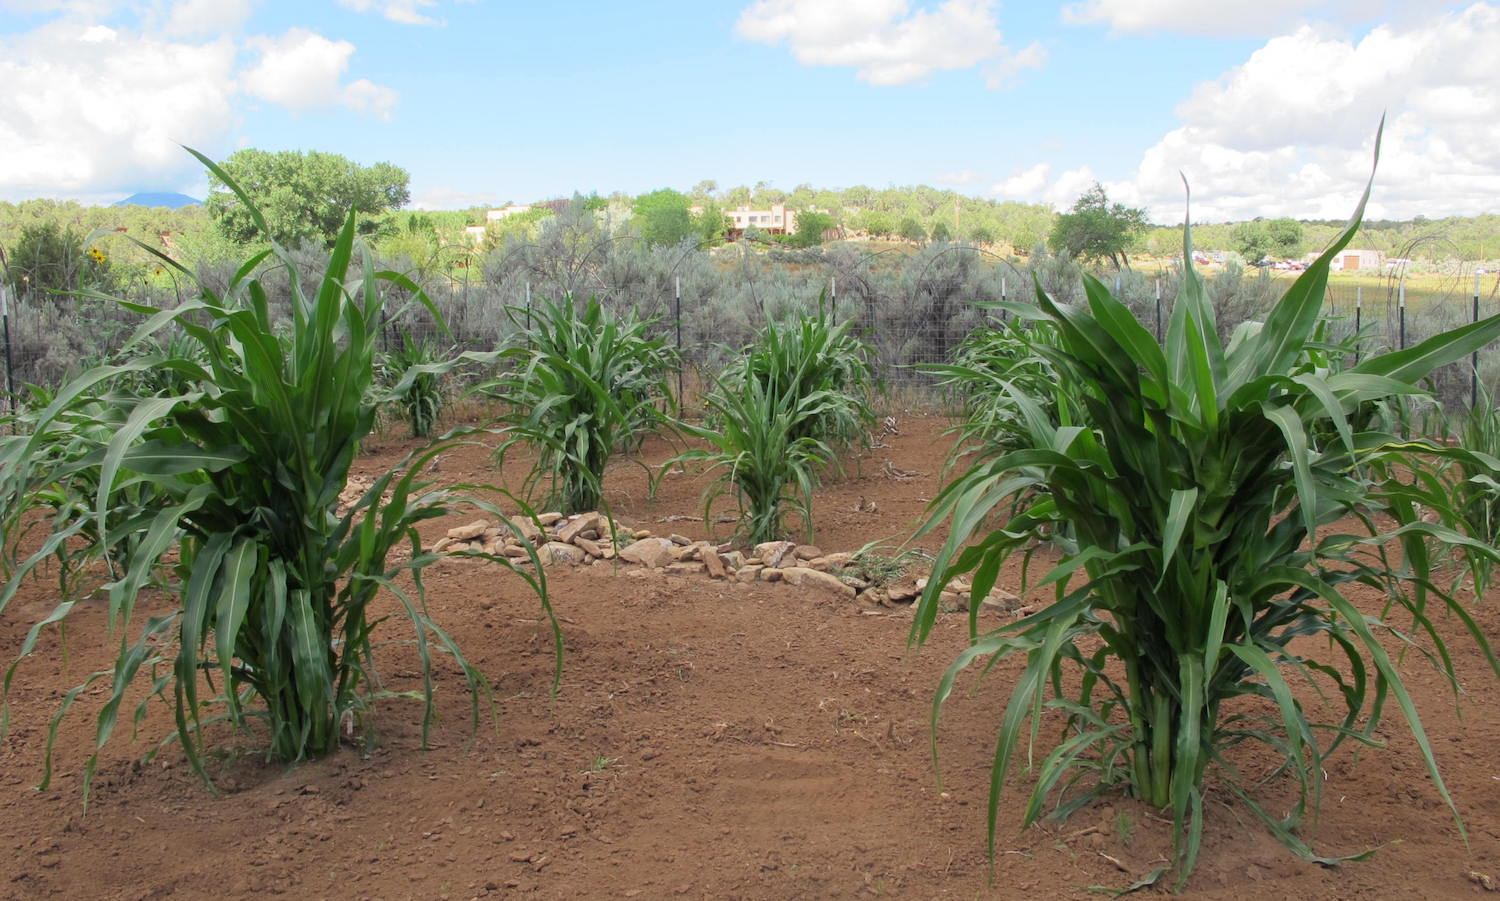
\includegraphics{./images/chapter_1_header.jpg}
\caption{A view from the Check Dam Garden.}
\end{figure}

\textbf{Farming is a fundamental part of Pueblo identity}. It is is integrated into every aspect of traditional Pueblo culture.

Pueblo leaders are concerned with preserving knowledge about farming and ensuring that this knowledge is transmitted to younger generations. Crow Canyon researchers and educators are interested in learning about traditional agriculture in order to better understand ancient farming practices and to gain a deeper appreciation for the role of corn in Pueblo society, past and present. \textbf{The Pueblo Farming Project} is a collaborative effort that addresses the interests of both groups.

Since 2006, the Crow Canyon staff has worked with traditional Pueblo farmers from Hopi, Arizona, to document their farming practices and the cultural context in which they take place. Every year, Hopi farmers have visited Crow Canyon in the spring and fall to teach the Center's researchers and educators about Pueblo Indian farming, food storage, and food preparation. Together, farmers and staff have planted and harvested several experimental gardens on Crow Canyon's campus, testing farming techniques and varieties of seeds used by the Pueblo farmers in their own fields.

Documentation for the project includes still photography, video, and audio recordings of planting and harvesting, and a variety of written records that include detailed measurements of plants at different stages of growth, daily temperature and precipitation values, crop yields, and preliminary results of corn DNA analysis. Data generated as part of the Pueblo Farming Project have already proven useful in broader research. For example, Village Ecodynamics Project scientists have compared the results of their computer simulations with corn harvest yields from the Pueblo Farming Project to better understand ancient environmental conditions and agricultural productivity---and the effects of both on human settlement patterns.

\hypertarget{what-was-the-pfp}{%
\subsection{What was the PFP?}\label{what-was-the-pfp}}

\hypertarget{history-of-the-pueblo-farming-project-20042018}{%
\subsubsection*{History of the Pueblo Farming Project: 2004--2018}\label{history-of-the-pueblo-farming-project-20042018}}
\addcontentsline{toc}{subsubsection}{History of the Pueblo Farming Project: 2004--2018}

\hypertarget{the-beginning}{%
\paragraph{The Beginning}\label{the-beginning}}
\addcontentsline{toc}{paragraph}{The Beginning}

The beginning of the Pueblo Farming Project can be traced to a September 2004 Native American Graves Protection and Repatriation Act (NAGPRA) consultation for Crow Canyon's Goodman Point Archaeological Project. National Park Service staff and Crow Canyon archaeologists met with Hopi Cultural Preservation Office staff at their office in Kykotsmovi, Arizona to discuss the research design for this project. When we concluded our discussion we asked the Hopi if there were research topics that interested them that were not covered in the research design, and they quickly responded that they wanted to know more about ancestral Pueblo farming and how it compared to the agricultural practices of Hopi and other Pueblo people today.

From these beginnings, the PFP has been developed through a partnership between Crow Canyon and Pueblo farmers, especially the farmers from Hopi whose participation in the project has been coordinated through the Hopi Cultural Preservation Office.

\hypertarget{designing-the-project}{%
\paragraph{Designing the Project}\label{designing-the-project}}
\addcontentsline{toc}{paragraph}{Designing the Project}

\begin{figure}
\centering
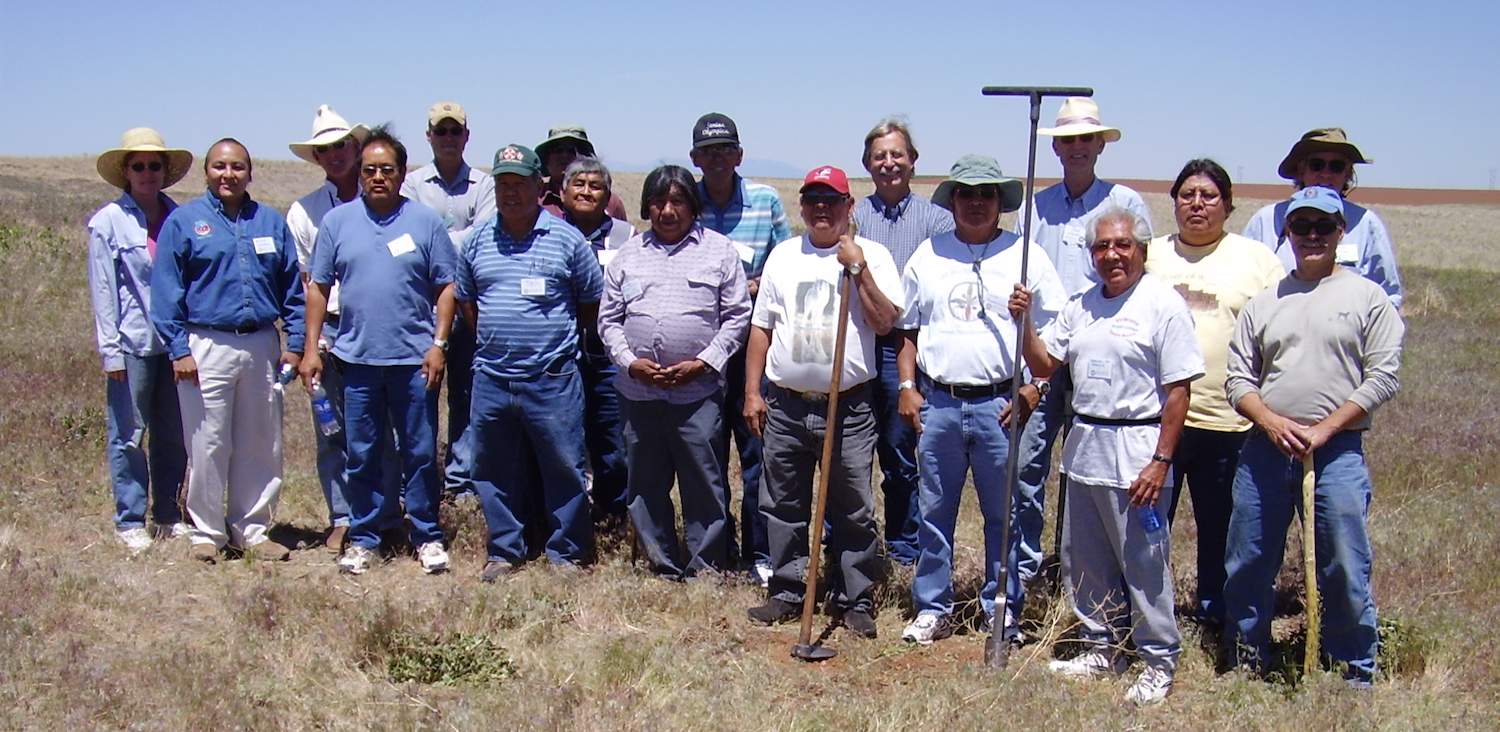
\includegraphics{./images/2006_group.jpg}
\caption{The participants in the May 2006 Pueblo farming planning meeting.}
\end{figure}

To follow through on this request, Crow Canyon developed the first of a series of grants to support a collaborative project on Pueblo farming (see section below on Who Funded the Pueblo Farming Project). The initial grant funded a planning meeting in May 2006 where we discussed the various types of research that could investigate ancestral Pueblo farming practices and link them to techniques used by modern Pueblo farmers. Participants at the meeting included traditional Pueblo farmers from Hopi, Jemez, Ohkay Owingeh, and Tesuque; Crow Canyon staff; and other anthropologists who specialize in the study of ancestral and modern Pueblo agriculture.

After two days of discussion, this group decided to implement an experimental gardening project that focused on direct-precipitation farming because this was the main type of farming practiced by the ancestral Pueblo in the Mesa Verde region. We use the term ``direct-precipitation farming'' to represent agricultural practices that use little to no large-scale landscape modification, but that readily take advantage of local landform and soil characteristics to enhance soil moisture (such as areas of higher runoff or greater snow accumulation) and often include small-scale anthropogenic modifications such as check dams. Direct-precipitation farming is sometimes referred to as ``dry-land'' or ``rain-fed'' farming. The group agreed that Hopi should take the lead as the traditional farming experts, since they still practice direct-precipitation farming whereas most other contemporary Pueblo tribes use more intensive flood-plain and canal irrigation techniques. Crow Canyon agreed to seek grant funding for the project that became known as the Pueblo Farming Project.

\hypertarget{selecting-garden-locations}{%
\paragraph{Selecting Garden Locations}\label{selecting-garden-locations}}
\addcontentsline{toc}{paragraph}{Selecting Garden Locations}

\begin{figure}
\centering
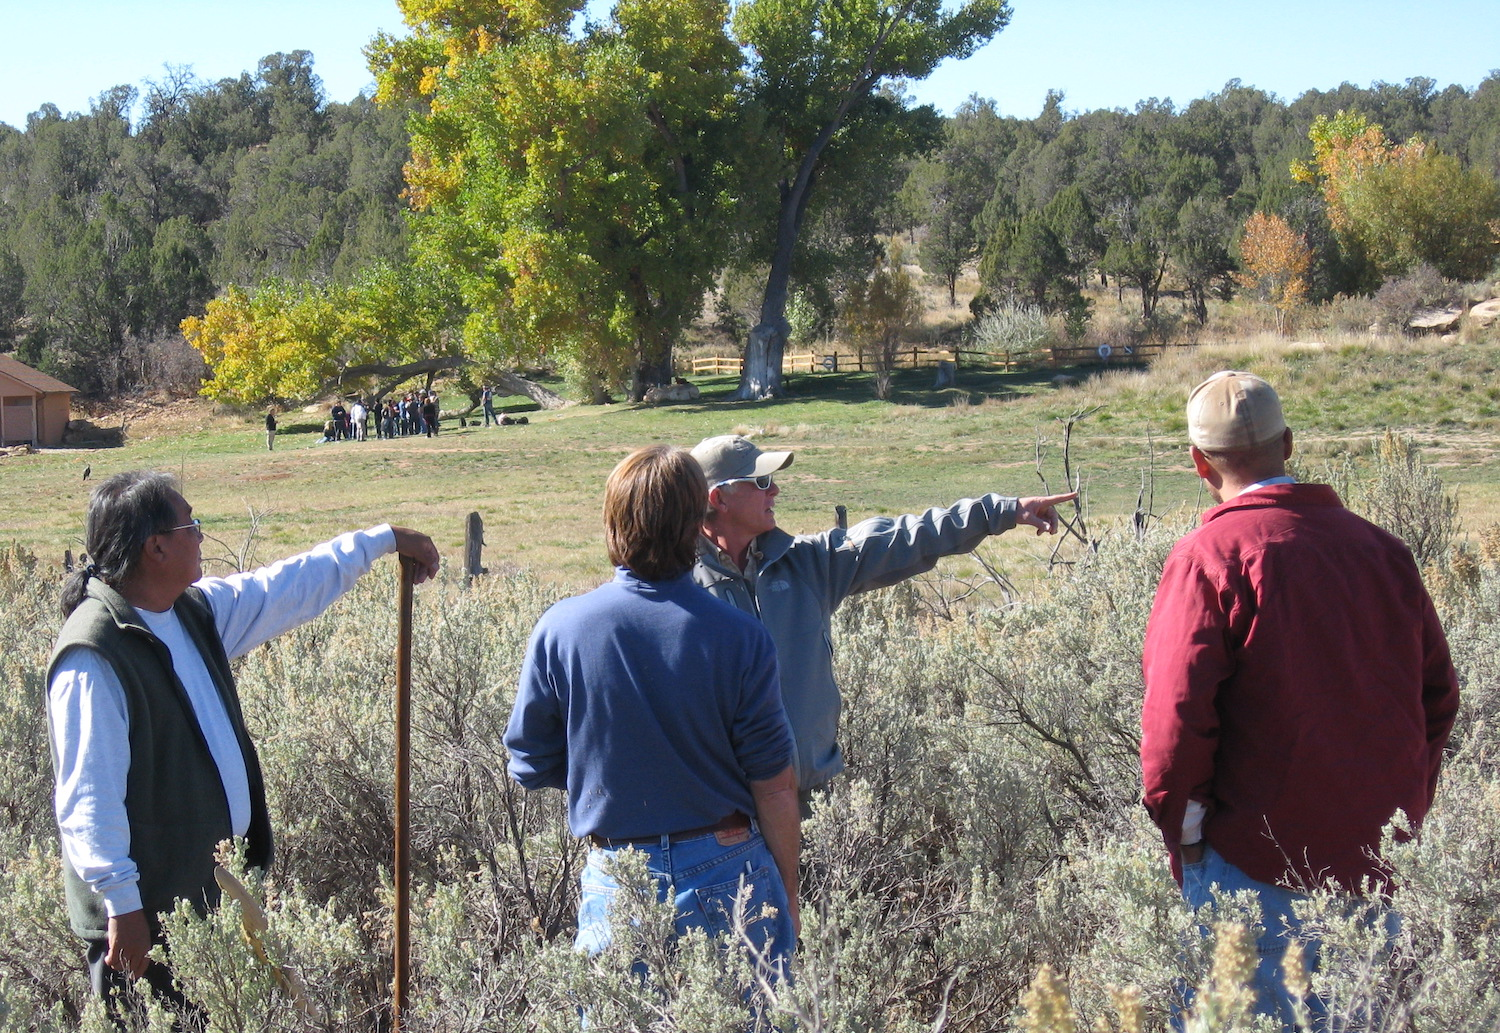
\includegraphics{./images/2007_locating_fields.jpg}
\caption{Locating fields during the 2007 PFP meetings.}
\end{figure}

The next step occurred in 2007 when Hopi farmers met to select locations for the gardens. We originally hoped to place these gardens at the Goodman Point Unit of Hovenweep National Monument to complement our ongoing research there, but we did not get permission for this and decided instead to locate the gardens on Crow Canyon's campus to integrate the PFP into the Center's education programs.

Pueblo farmers used traditional ecological knowledge to select the garden locations, focusing on the native plants that indicate good areas for farming. Rabbitbrush and snakeweed are two plants they see as indicating prime areas, but dense stands of those plants were not present on Crow Canyon's campus. In the absence of such indicator species, they selected two areas in small washes on the east side of Crow Canyon that are dominated by sagebrush today. The sagebrush in these areas was taller because their location in small drainages provided more moisture than the areas outside the drainages. The farmers assessed soils for their texture and moisture-holding capacity and examined the details of specific settings including slope, aspect, and other factors. Although the Hopi farmers did not consider these two locations as ideal, they thought they would be adequate.

One location had sage that was unusually tall; this area was located near the mouth of a small wash coming from the east slope of the Crow Canyon drainage. When this area was cleared, an ancient check dam was found and subsequently recorded (5MT19690). This was named the Check Dam Garden (CDG). The other plot was located higher up in a small drainage to the north in an area where there was a thick patch of verdant grass. The Hopi farmers thought there might be a spring in this area but subsequent work showed this was not the case. We call this plot the Pueblo Learning Center (PLC) garden because it is on the way to one of Crow Canyon's outdoor classrooms.

In addition to these new plots, the Hopi farmers suggested we continue planting a garden that Paul Ermigiotti had earlier developed for Crow Canyon's educational programs. We call this Paul's Old Garden (POG), and it is located on the valley floor in the bottom of Crow Canyon.

In 2009, we added two additional garden areas. The first, the Pithouse garden (PHG), was placed on the west slope of Crow Canyon and adjacent to Crow Canyon's Pithouse Learning Center to incorporate the garden into the lessons that occur there. The PHG garden had anomalously low yields for several years and soil profiles showed that the area had been disturbed when the adjacent replica pithouse was constructed (the garden soils contained construction materials), so we abandoned this garden after the 2014 growing season.

\begin{figure}
\centering
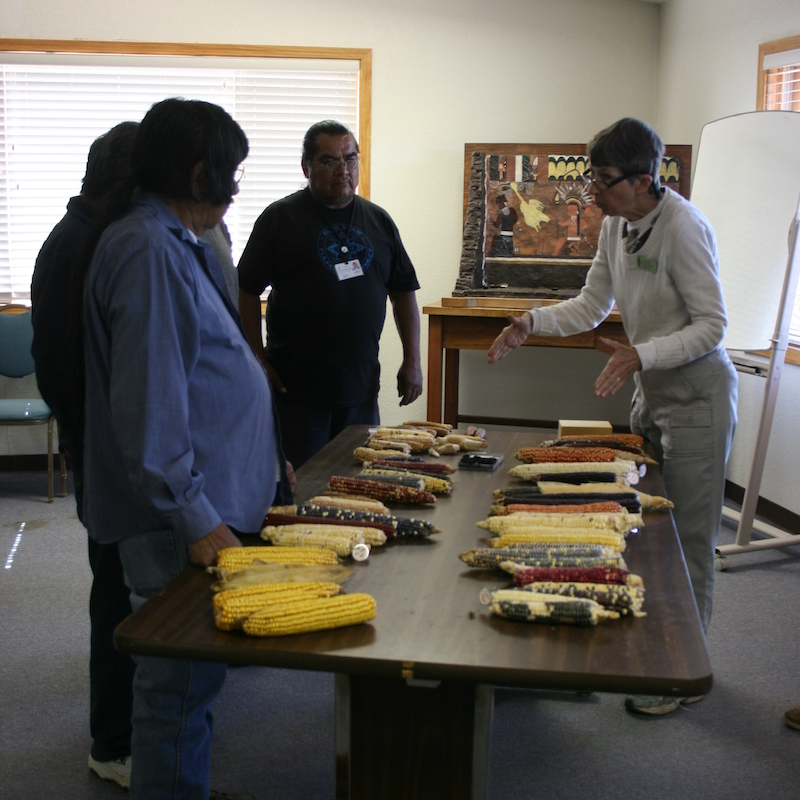
\includegraphics{./images/karen_and_hopi.jpg}
\caption{Karen Adams and Hopi farmers discussing variation in corn.}
\end{figure}

The second garden added in 2009 was Karen's Upper Garden (KUG), which was a plot farmed by Karen Adams in the 1990s and located on the mesa just west of Crow Canyon. Karen farmed this garden as part of Crow Canyon public education program and to quantify yields. Karen's Upper Garden has produced relatively low yields, which surprised us because evidence suggests that the mesa tops covered in Mesa Verde loess-derived soils were the area most intensively farmed by ancestral Pueblo people. This evidence includes the fact that most ancestral Pueblo habitation sites are near these loess soils on the mesa tops, and the fact that these loess-derived, mesa-top soils are the focus of contemporary direct-precipitation farming. To better evaluate the variation in these mesa-top settings, we added an additional garden in 2015 at Mike Coffey's farm near Dove Creek, Colorado (the Mike Coffey Garden or MCG).

The \protect\hyperlink{where-did-the-pfp-take-place}{PFP garden locations} allow us to measure the effect of a variety of microenvironmental factors on agricultural potential. For example, the Crow Canyon gardens allow us to evaluate the effect of cold air that flows in drainages. The length of the frost-free period varies considerably despite relatively small differences in elevation and in the distance between the plots. The gardens are also located on soils with different characteristics and the effects of soil variability are the primary focus of this study.

\hypertarget{planting-and-harvesting-20082018}{%
\paragraph{Planting and Harvesting: 2008--2018}\label{planting-and-harvesting-20082018}}
\addcontentsline{toc}{paragraph}{Planting and Harvesting: 2008--2018}

\begin{figure}
\centering
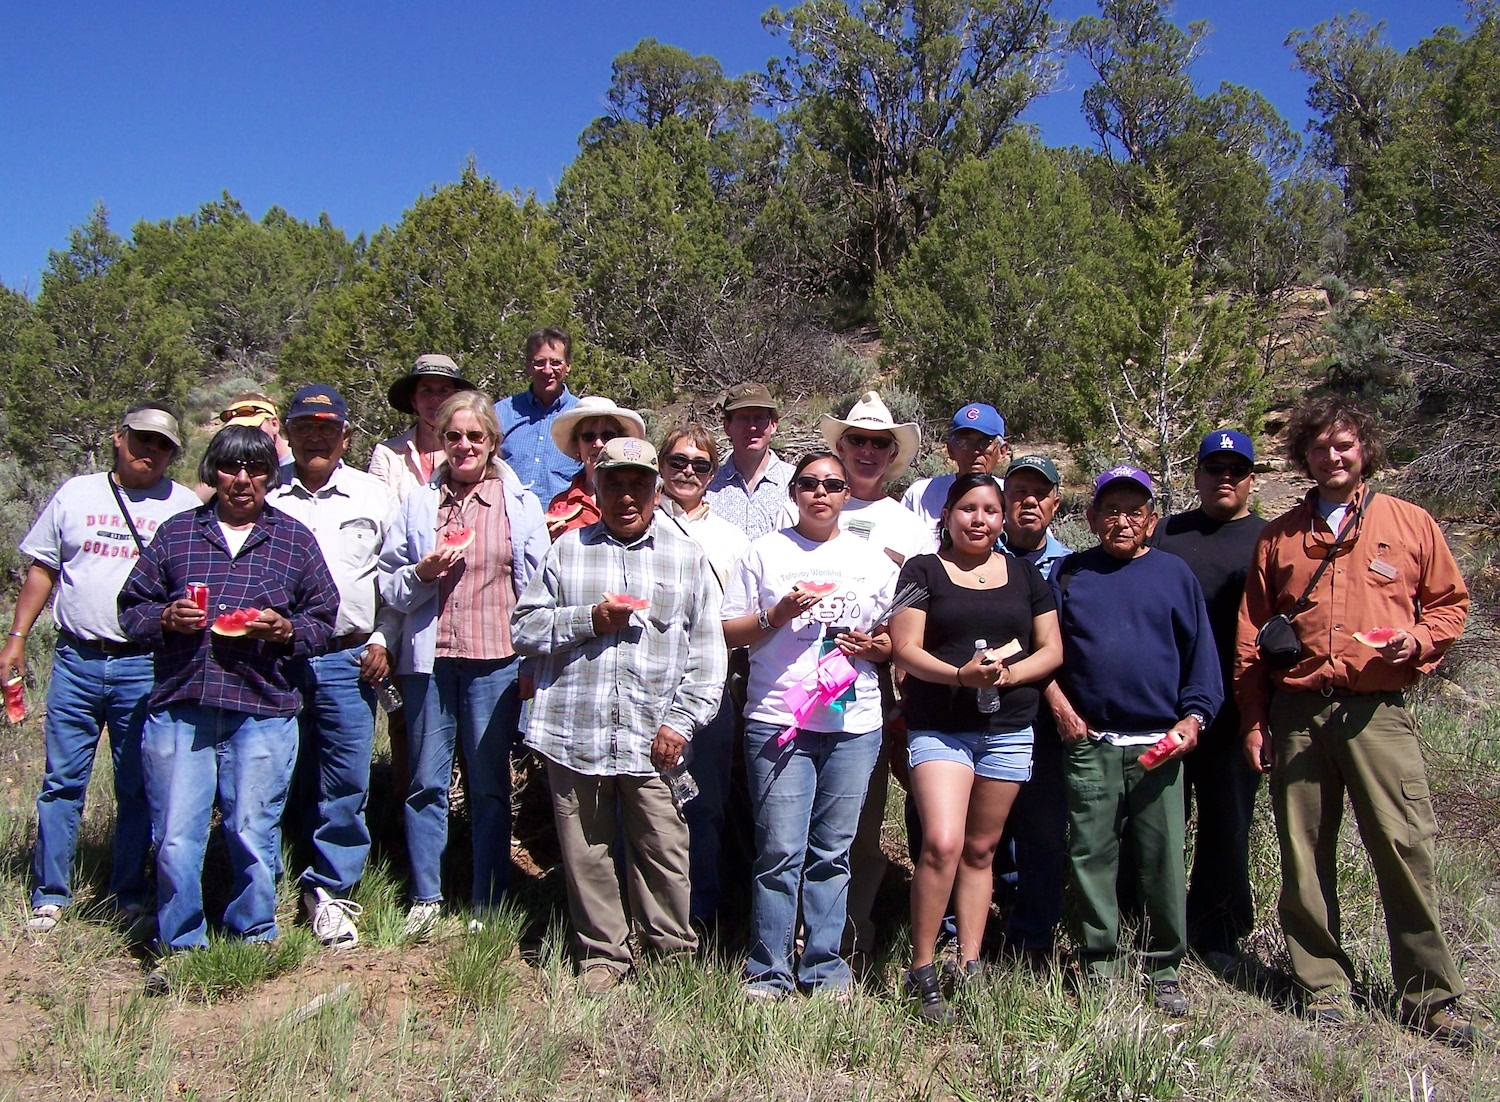
\includegraphics{./images/2008_planting_fields.jpg}
\caption{The participants in the initial planting of the PFP gardens in 2008.}
\end{figure}

We planted and harvested gardens for the first time in 2008, with the work focused on the Check Dam Garden, Pueblo Learning Center garden, and Paul's Old Garden. From 2009--2014 we planted five gardens: the Check Dam Garden, Pueblo Learning Center garden, Paul's Old Garden, Pit House Garden, and Karen's Upper Garden. From 2015--2018 we planted the Check Dam Garden, Pueblo Learning Center garden, Paul's Old Garden, Karen's Upper Garden, and Mike Coffey Garden. During this time, Pueblo farmers served as the expert consultants for planting and harvesting. Most of the farmers are from Hopi, but farmers from other Pueblos have also participated. Crow Canyon staff members learn from the Pueblo farmers and assist in the planting and harvesting.

\hypertarget{pueblo-farming-project-goals}{%
\paragraph{Pueblo Farming Project Goals}\label{pueblo-farming-project-goals}}
\addcontentsline{toc}{paragraph}{Pueblo Farming Project Goals}

\begin{figure}
\centering
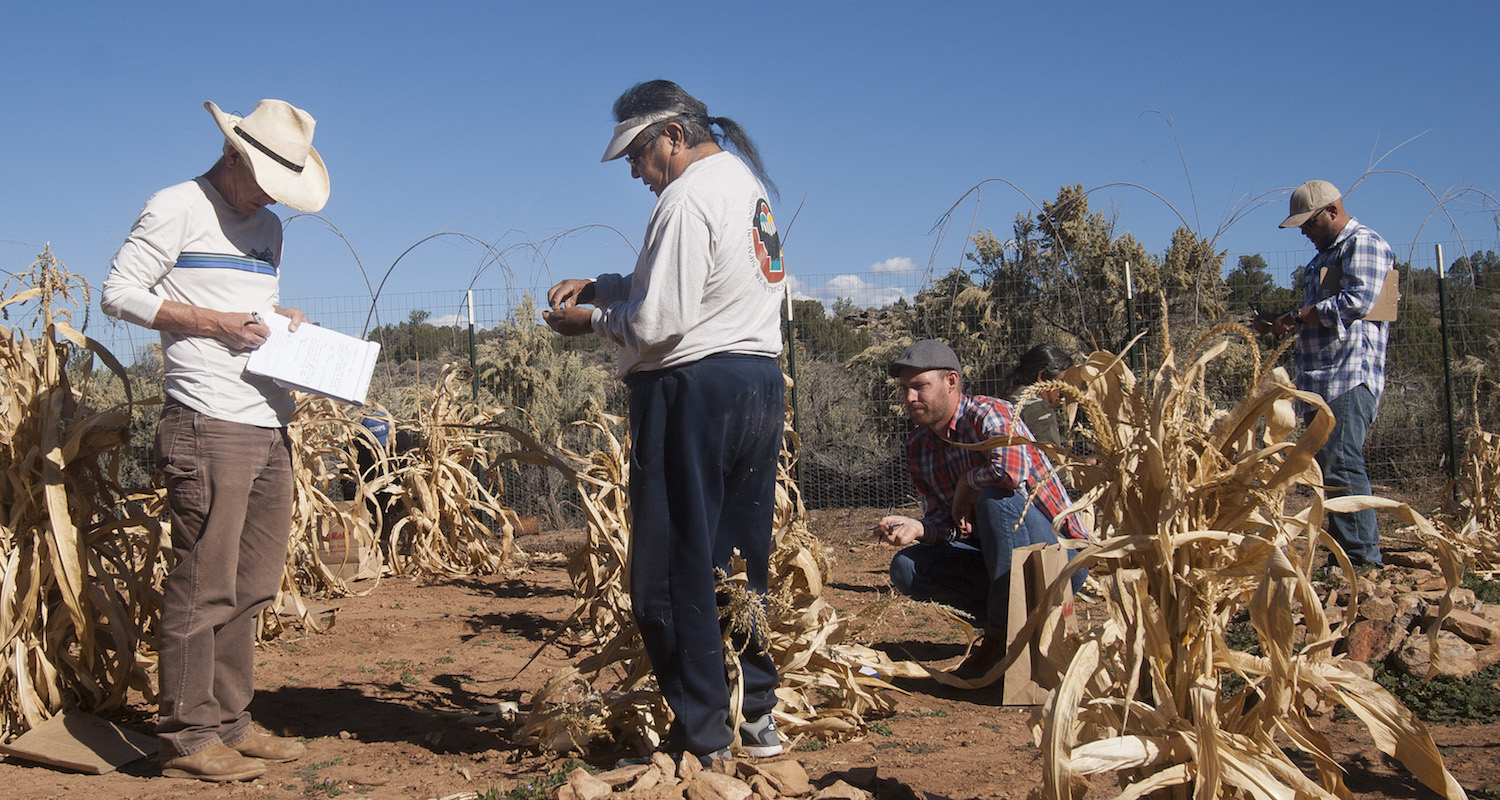
\includegraphics{./images/harvesting_2.jpg}
\caption{Harvesting and recording maize in 2016.}
\end{figure}

From the beginning, the Pueblo Farming Project has pursued educational and research goals that were developed by Hopi and Crow Canyon working together. Since 2008, Hopi farmers have traveled to Crow Canyon twice a year: once in the spring for a planting meeting and again in the fall for a harvest meeting. Each meeting includes discussions to review goals, evaluate the project's progress, and develop a plan for how to proceed with current and future initiatives. Of course, each meeting also includes work in the agricultural plots.

All Pueblo Farming Project activities have been recorded using numerous techniques: written notes from each meeting, audio and video recording, still photography, and written documentation that include detailed metrics on the plants and their growing environments. This has produced a rich dataset from which we produced several research and educational products.

\begin{figure}
\centering
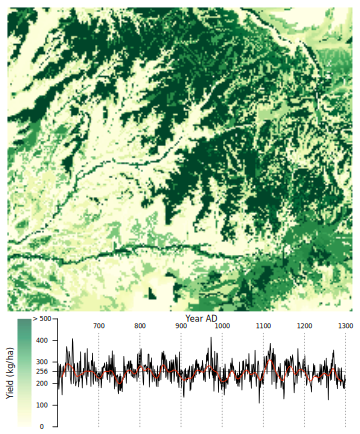
\includegraphics{./images/vep.svg}
\caption{The Village Ecodynamics Project maize productivity estimates, AD 600--1300. The map panel (top) shows the average yield across time (in kilograms per hectare, kg/ha). The graph panel (bottom) is the average yield across space, through time. The black line represents the annual average; the red line smooths the annual data to show long-term trends.}
\end{figure}

One of the Pueblo Farming Project research goals was to evaluate how agricultural yields were affected by annual variation in temperature and precipitation. These data were integrated into another research project known as the Village Ecodynamics Project or VEP. The Village Ecodynamics Project was funded by two National Science Foundation grants awarded to Washington State University; Crow Canyon was a subcontractor on the project. A multidisciplinary collaboration, the Village Ecodynamics Project included archaeologists, geologists, hydrologists, geographers, computer scientists, and economists from institutions across the US and Canada. Village Ecodynamics Project researchers studied the interaction between Pueblo Indian people and their environment over more than a thousand years, beginning in AD 600. One aspect of the Village Ecodynamics Project was to use computer modeling to estimate ancestral Pueblo agricultural yields and how they varied through time and across the project study areas. Actual Pueblo Farming Project yields were compared to the Village Ecodynamics Project estimates to evaluate the accuracy of the computer model. Detailed information about the Village Ecodynamics Project can be found at this website: \url{http://www.veparchaeology.org/}.

Hopi goals for the project were tied to the central role of corn and corn farming in Hopi culture. Fundamentally, they were interested in whether their seed and their traditional farming techniques would result in successful harvests in the Mesa Verde region, a place they consider as part of their ancestral homeland. For Hopi, the Pueblo Farming Project provided a substantive link between their past and the present. For Hopi, the Pueblo Farming Project helped demonstrate their cultural affiliation to the Mesa Verde region, and beyond planting and harvesting gardens they pursued this goal through another Pueblo Farming Project research initiative: the DNA analysis of modern Hopi corn.

\hypertarget{education-products}{%
\paragraph{Education Products}\label{education-products}}
\addcontentsline{toc}{paragraph}{Education Products}

\begin{figure}
\centering
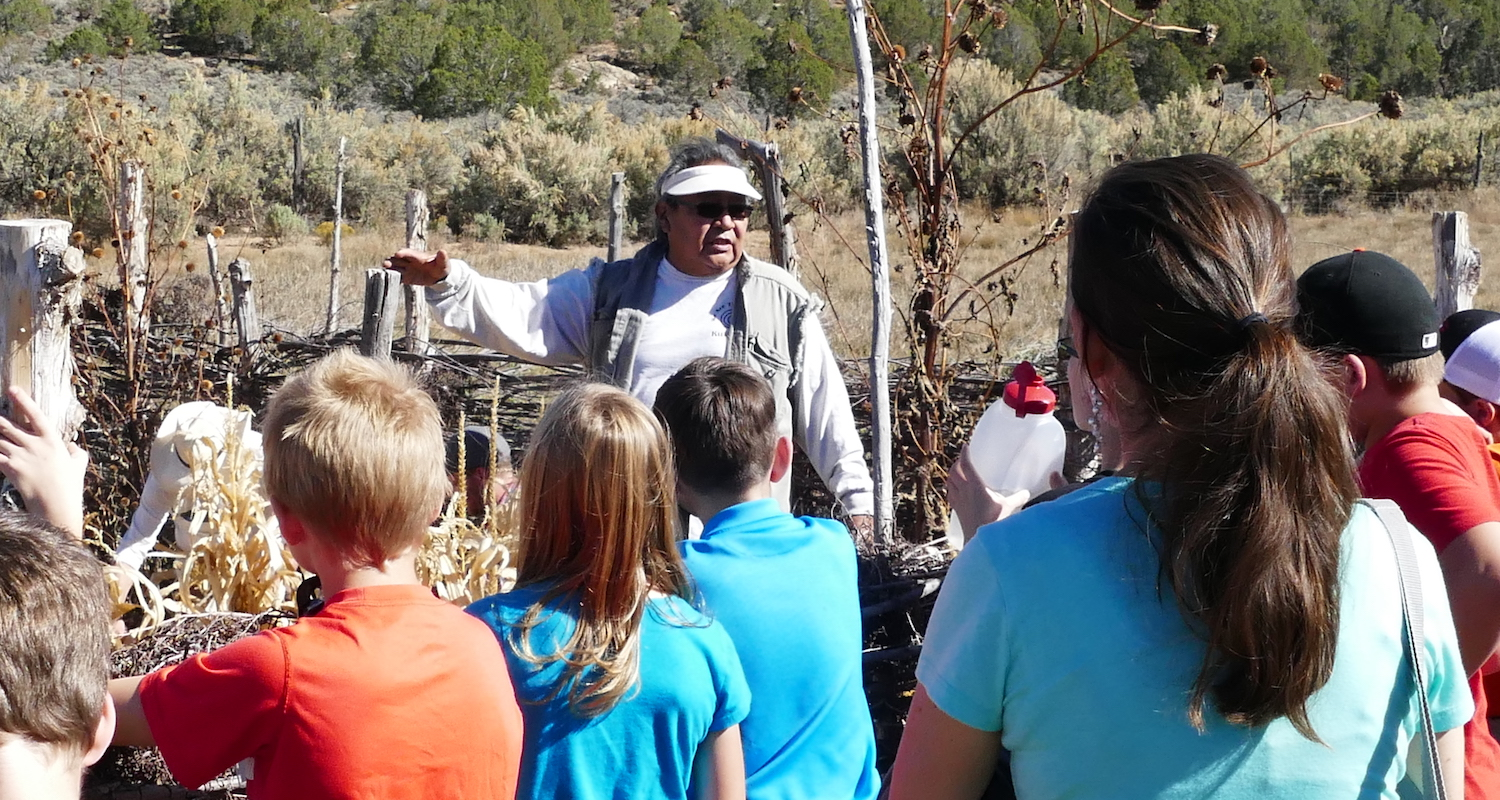
\includegraphics{./images/children.jpg}
\caption{School children learning about Hopi farming.}
\end{figure}

From the beginning, the Pueblo Farming Project was integrated into Crow Canyon's education programs. School groups who are at Canyon when planting and harvesting occurs observe and at times participate in these activities. Pueblo farmers speak to the students about the project and the role of farming in Pueblo culture, creating a unique and memorable learning experience for these students. The Pueblo Farming Project gardens are also integrated into Crow Canyon education programs during the growing season, providing the students with a powerful visual as the Center's educators teach about the importance of corn farming in ancestral and modern Pueblo communities.

\begin{figure}
\centering
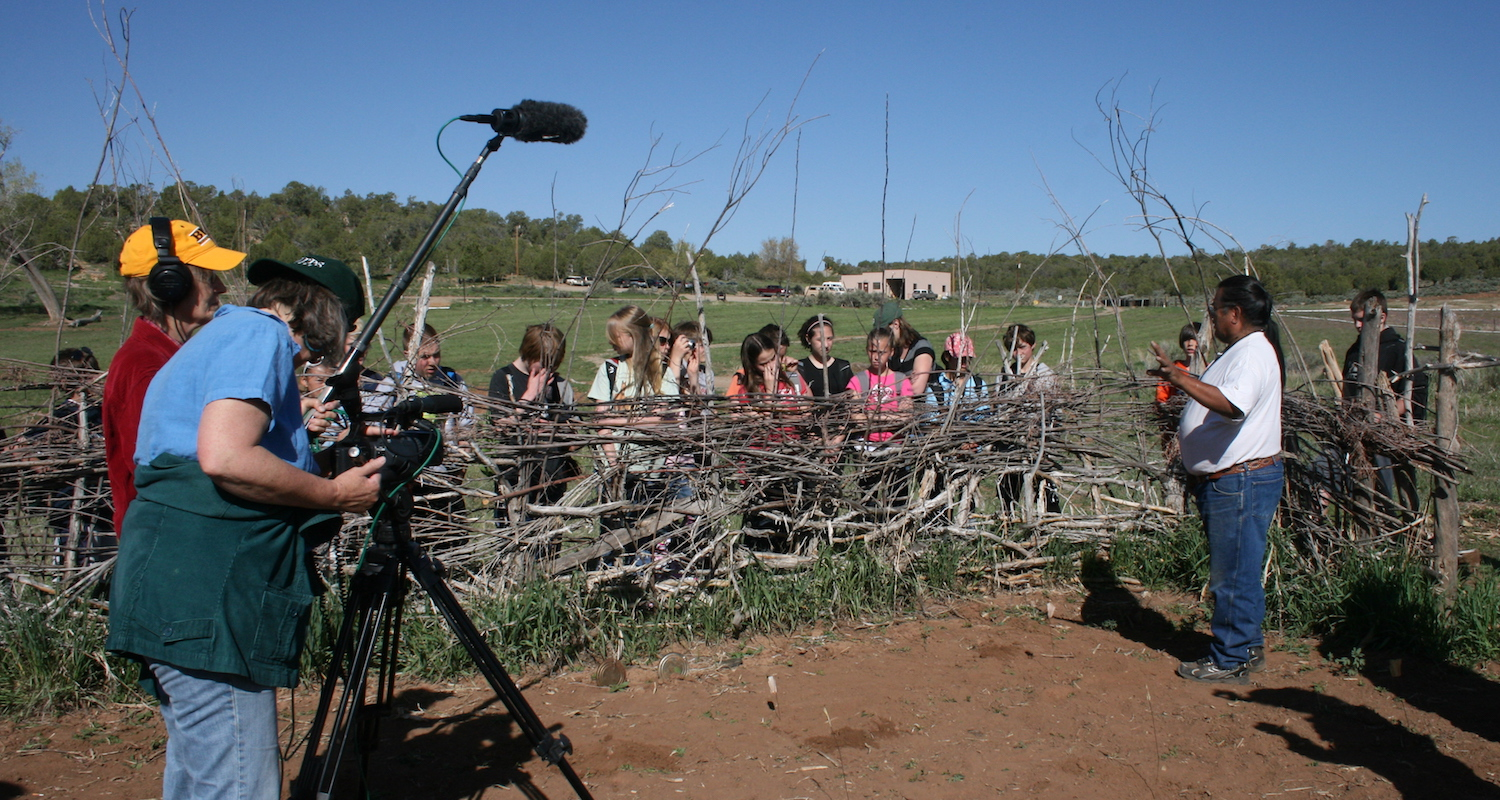
\includegraphics{./images/section_1.1_documentary.jpg}
\caption{Filming the documentary `More than Planting a Seed'.}
\end{figure}

We also developed series of educational initiatives to reach a larger audience with what we have learned through the Pueblo Farming Project. We highlight three of these initiatives here. The first educational product we highlight is a documentary film, \emph{More than Planting a Seed}:

A second educational product is an exhibit on display at the Crow Canyon Archaeological Center. This exhibit describes the project, presents our results, and tells the story of corn. Finally, we created and piloted five standards-aligned lessons for the classroom. Those lessons plans are included in this eBook.

Public education initiatives also include lectures for the public and presentations at professional meetings. Information about the Pueblo Farming Project was also disseminated through Crow Canyon's electronic and print newsletters and on Crow Canyon's website. The Pueblo Farming Project was also featured on local radio shows, including \href{http://ksjd.org/post/pueblo-farming-project\#stream/0}{an interview with Leigh Kuwanwisiwma on KSJD's Big Fat Farm Show}.

\hypertarget{who-were-the-participants}{%
\subsection{Who were the participants?}\label{who-were-the-participants}}

\begin{figure}
\centering
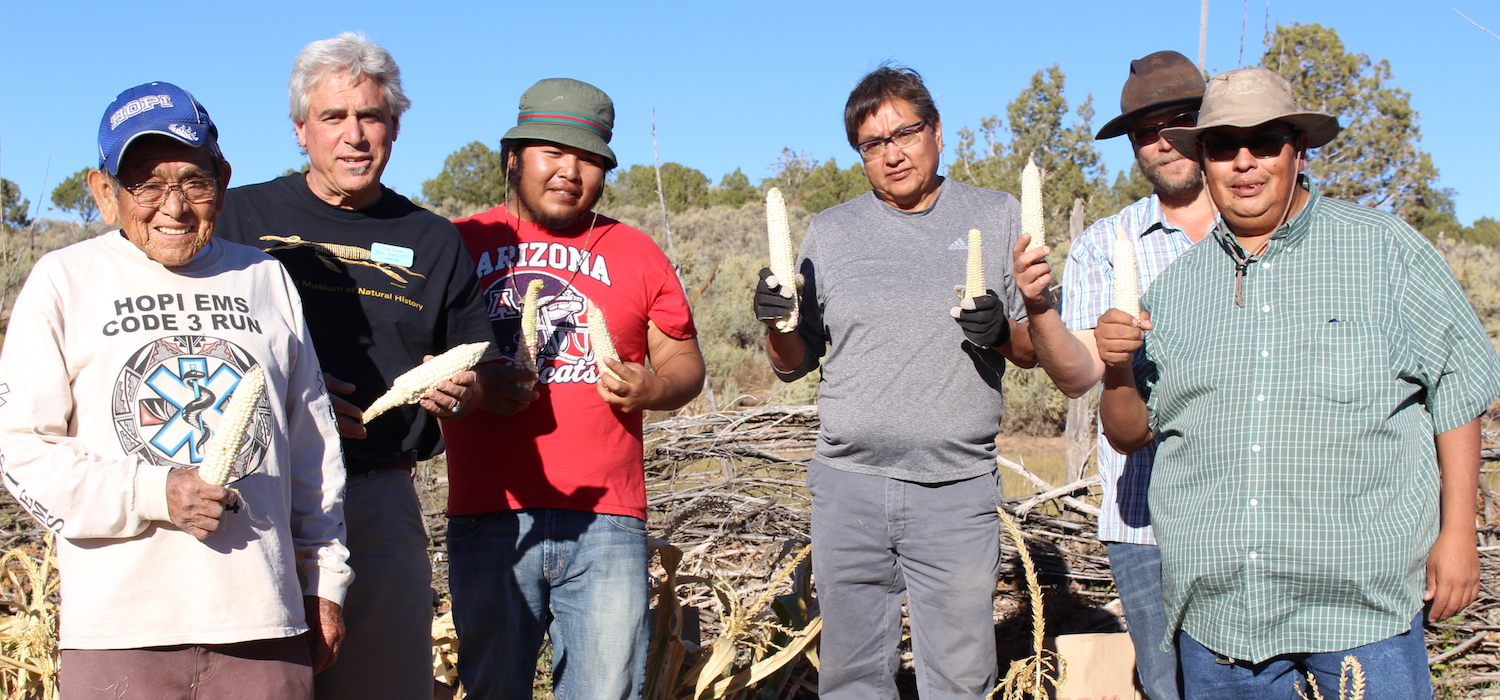
\includegraphics{./images/section_1.2_header.jpg}
\caption{Harvesting the Pueblo Farming Project gardens.}
\end{figure}

Over almost a decade, dozens of Hopi farmers, researchers, and volunteers participated in the Pueblo Farming Project, and hundreds of students visited the Pueblo Farming Project gardens during the growing season.

~

\hypertarget{where-did-the-pfp-take-place}{%
\subsection{Where did the PFP take place?}\label{where-did-the-pfp-take-place}}

\begin{figure}
\centering
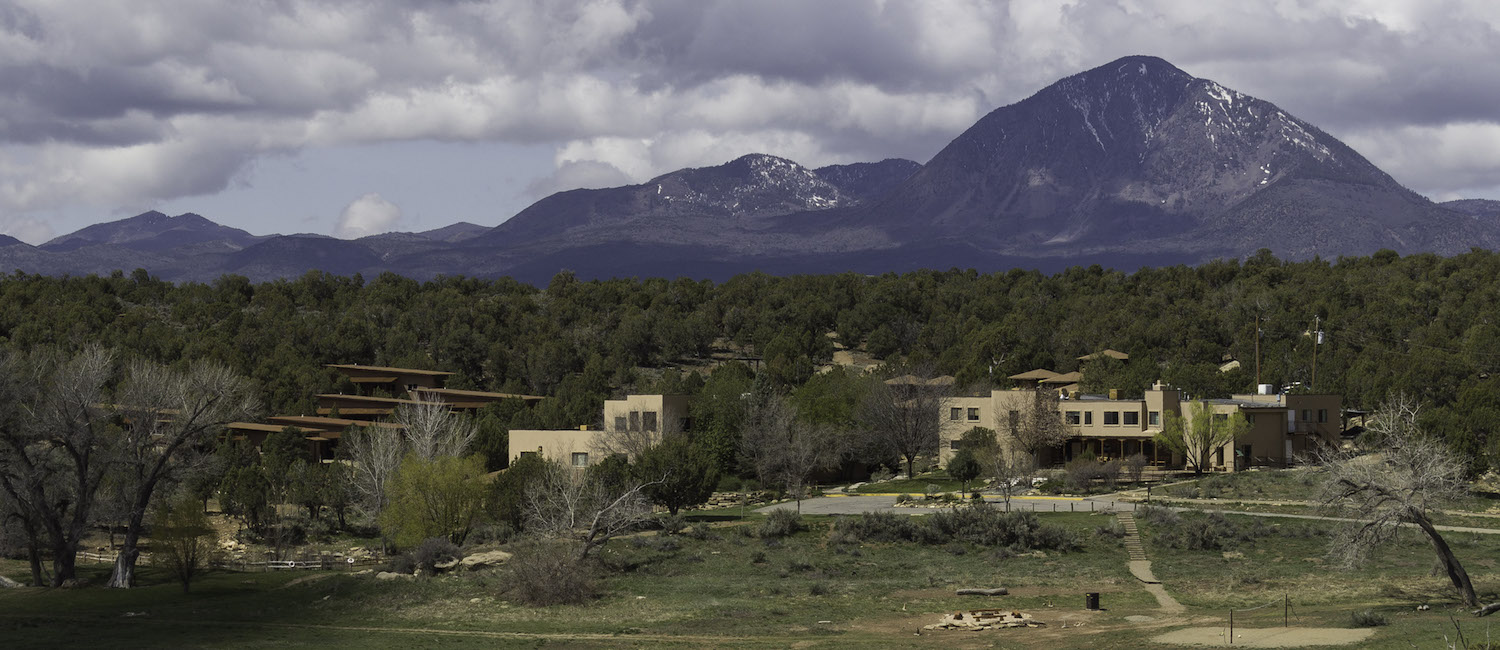
\includegraphics{./images/section_1.3_header.jpg}
\caption{Crow Canyon Archaeological Center's rural campus in Cortez, Colorado.}
\end{figure}

Five Pueblo Farming Project gardens are scattered around Crow Canyon Archaeological Center's rural campus in Cortez, Colorado. In 2015, we planted a new garden in the contemporary dry-farmed region north of Crow Canyon's campus. Use the map below to explore the PFP garden locations, and click on the gardens to get more information about when they were planted as part of Pueblo Farming Project research. You can zoom using the controls on the left, the scrollwheel on your mouse, or by pinching on a mobile device. The menu in the upper right allows for different map backgrounds. The mapped boundaries of each garden are at the garden fences; gardens may not have been completely planted in each year.


\includegraphics{images/unnamed-chunk-1-1.pdf}

\hypertarget{who-funded-the-pfp}{%
\subsection{Who funded the PFP?}\label{who-funded-the-pfp}}

The Pueblo Farming Project started as part of the Village Ecodynamics Project and was initially funded under National Science Foundation grants DGE-1347973 and DEB-0816400. Subsequent years of the Pueblo Farming Project received funding from the History Colorado State Historical Fund (grant 2015-02-025), the National Geographic Society Genographic Project, and the Christensen Fund.

\hypertarget{the-story-of-maize}{%
\section{The Story of Maize}\label{the-story-of-maize}}

\begin{figure}
\centering
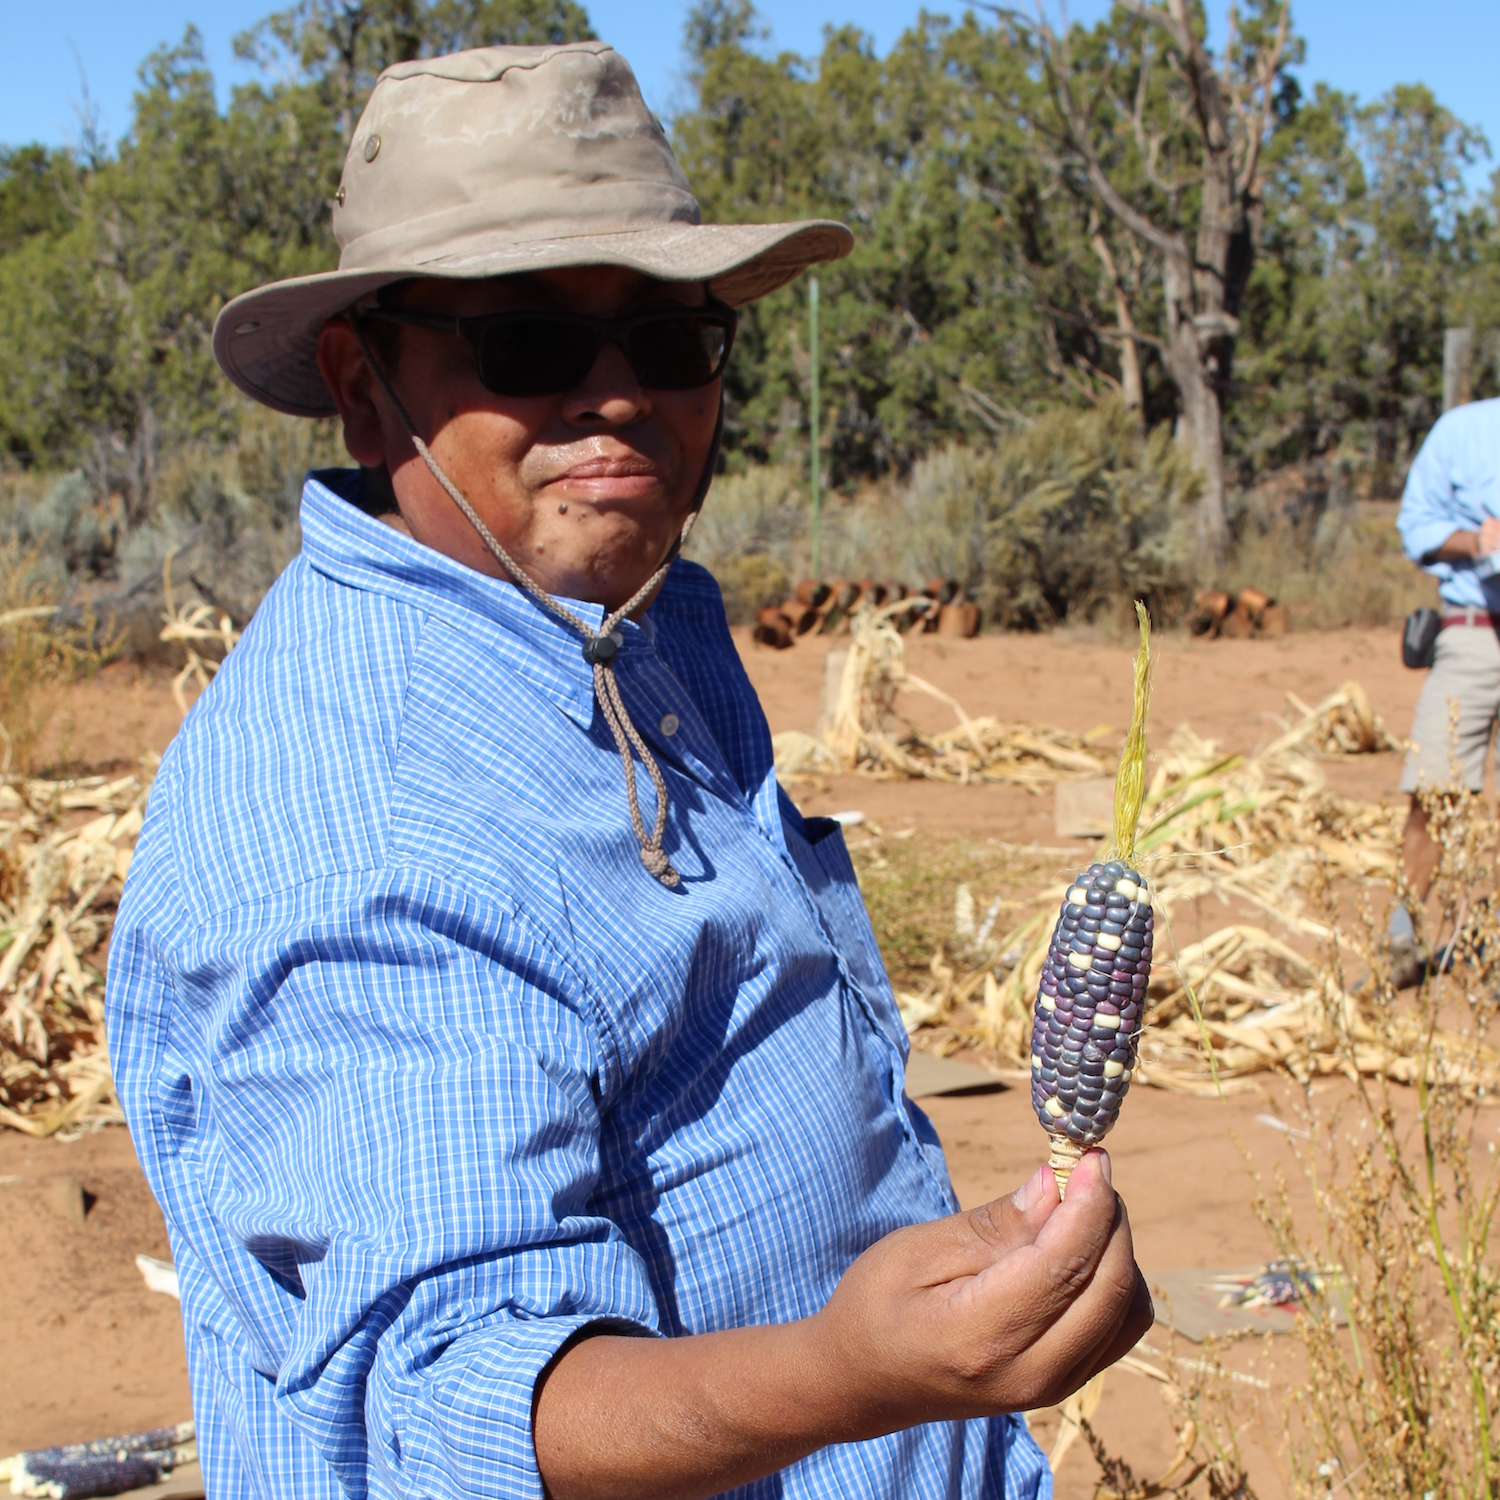
\includegraphics{./images/chapter_2_header.jpg}
\caption{Harvesting the small blue ear like the one Masau'u provided the Hopi people.}
\end{figure}

The relationship between humans and corn (or maize, \emph{Zea mays} ssp. mays) is a long and interesting story. The path to domestication began about 9,000 years ago in southwestern Mexico. The domestication process led to a unique codependency: as it exists today, corn is not able to reproduce without human intervention. But humans have also become dependent upon this plant.

Today, corn is the most widely produced grain crop in the United States, though only a tiny fraction of the corn grown directly feeds people. Most of what we consume is in the form of high-fructose corn sweeteners. Most corn production goes toward animal feed, ethanol and exports. Corn has become less of an important food resource and more of a refined industrial product. In contrast, corn holds an important place in the origin myths and lifeways of many native cultures. In Pueblo cultures, maize plays a vital position physically, spiritually, and symbolically.

\begin{figure}
\centering
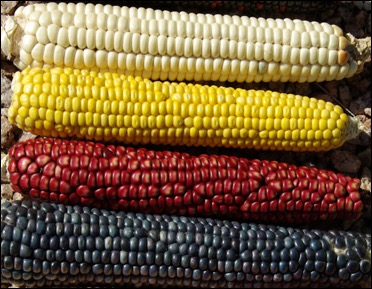
\includegraphics{./images/directional_corn.jpg}
\caption{Corn as directional symbols: white---northeast, yellow---northwest, red---southeast, blue---southwest.}
\end{figure}

\hypertarget{origins}{%
\subsection{Origins}\label{origins}}

\begin{figure}
\centering
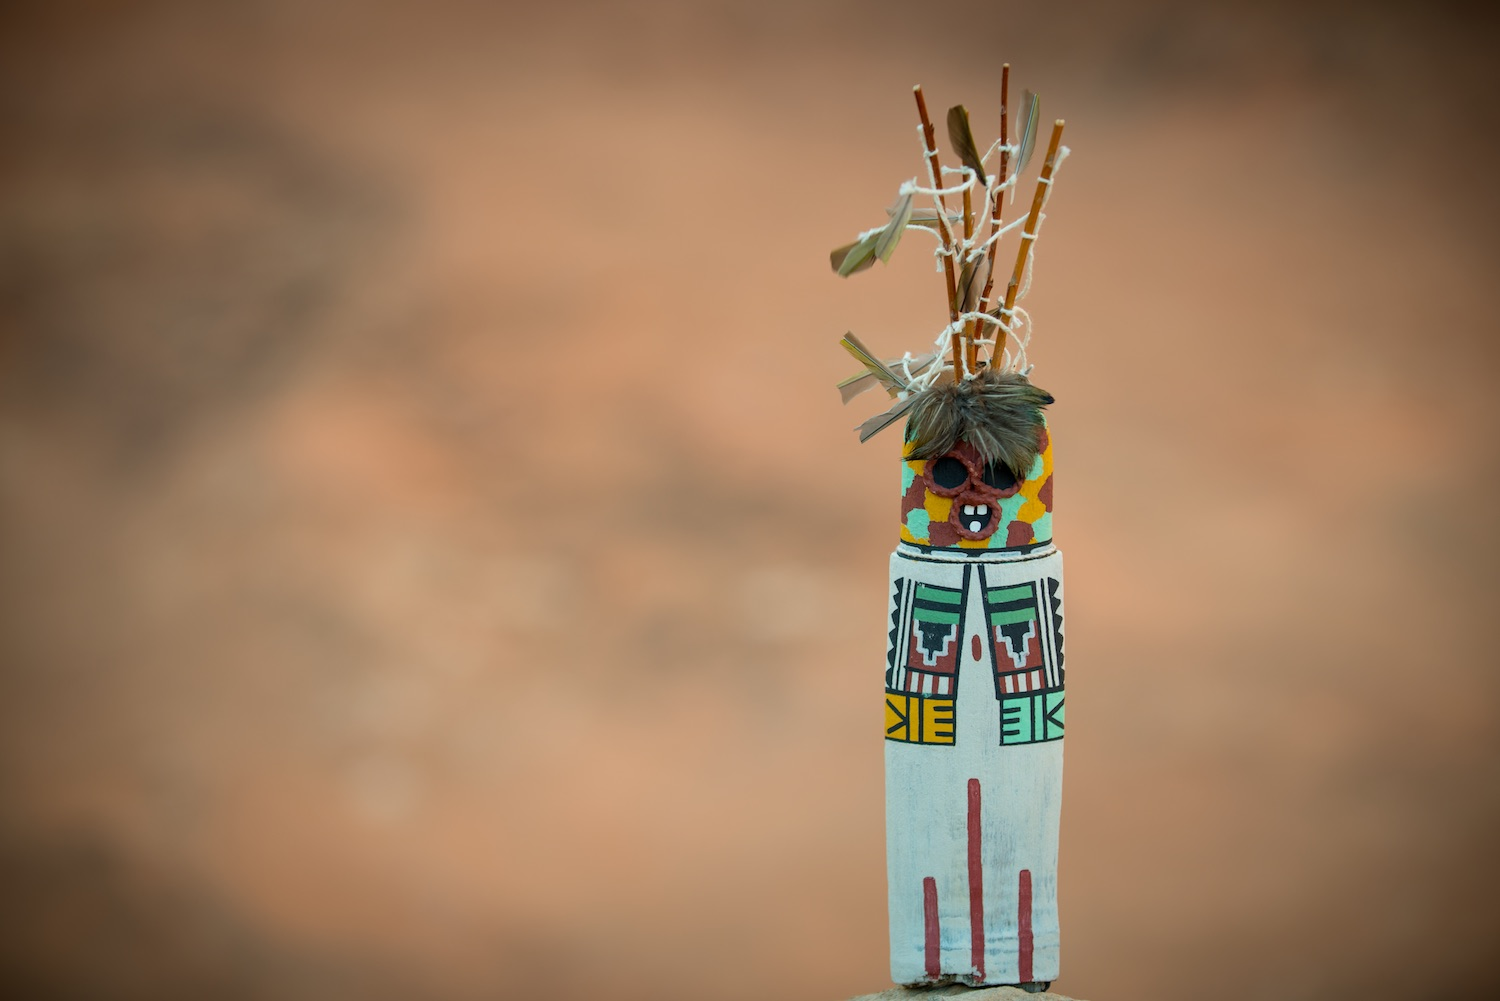
\includegraphics{./images/section_2.1_origin.jpg}
\caption{A Hopi \emph{tihu} or representational figurine, depicting Masau'u.}
\end{figure}

The domestication of maize was unique. Typically, domesticated plants look similar to their wild ancestors; However, an ear of corn's closest wild relative, teosinte, is noticeably different from an ear of modern corn. An ear of maize is wrapped in a husk and the kernels are held tightly and not able to scatter or free themselves from the cob, whereas the kernels of teosinte are able to scatter freely. Because the husks of corn must be removed in order for corn to reproduce, corn is as dependent on humans as humans are dependent on corn.

Teosinte, a wild grass native to Mexico and Central America, is so closely related to maize that it belongs to the same species, \emph{Zea mays}, but is a different subspecies: parviglumis. Despite their shared ancestry, the plants differ in significant ways:

\begin{longtable}[]{@{}ll@{}}
\toprule
\begin{minipage}[b]{0.47\columnwidth}\raggedright
\textbf{Maize}\strut
\end{minipage} & \begin{minipage}[b]{0.47\columnwidth}\raggedright
\textbf{Teosinte}\strut
\end{minipage}\tabularnewline
\midrule
\endhead
\begin{minipage}[t]{0.47\columnwidth}\raggedright
grows as a single stalk with a few large ears\strut
\end{minipage} & \begin{minipage}[t]{0.47\columnwidth}\raggedright
branched with many small ears\strut
\end{minipage}\tabularnewline
\begin{minipage}[t]{0.47\columnwidth}\raggedright
ears are encased in a husk with hundreds of kernels on the cob\strut
\end{minipage} & \begin{minipage}[t]{0.47\columnwidth}\raggedright
ears have eight to 12 kernels, each surrounded by a hard fruit-case\strut
\end{minipage}\tabularnewline
\begin{minipage}[t]{0.47\columnwidth}\raggedright
ears typically have 8 to 16 rows of kernels\strut
\end{minipage} & \begin{minipage}[t]{0.47\columnwidth}\raggedright
ears have two rows of kernels\strut
\end{minipage}\tabularnewline
\begin{minipage}[t]{0.47\columnwidth}\raggedright
kernels must be separated from the ear and planted by humans\strut
\end{minipage} & \begin{minipage}[t]{0.47\columnwidth}\raggedright
ears shatter when dry and the seeds scatter, distributed by gravity, birds and other animals\strut
\end{minipage}\tabularnewline
\bottomrule
\end{longtable}

\hypertarget{the-people-of-corn}{%
\subsection{The people of corn}\label{the-people-of-corn}}

\begin{figure}
\centering
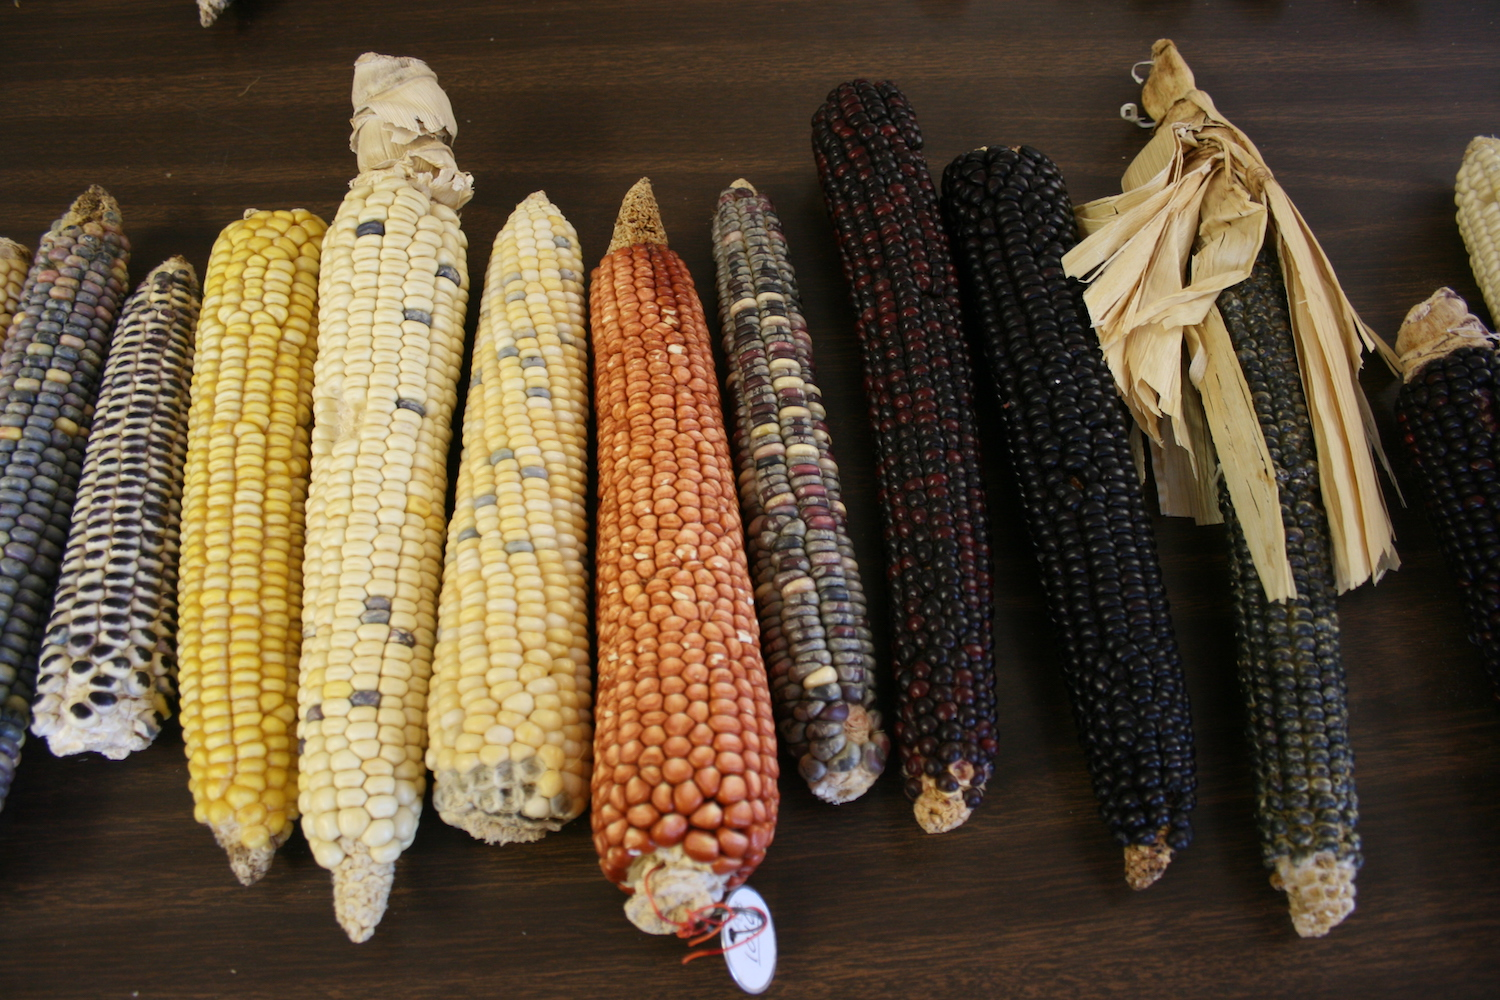
\includegraphics{./images/varieties.jpg}
\caption{Varieties of maize.}
\end{figure}

Maize entered the southwestern United States about 4,000 years ago. On its long journey from Mexico, maize has adapted from its tropical environment, which has 12 hours of daylight, to the semiarid, long summer days and cool night conditions of the Colorado Plateau. Farming techniques also had to adapt. Direct-precipitation agriculture is dependent on moisture stored in the soil from precipitation and runoff water. Pueblo people have practiced direct-precipitation farming in the arid Southwest for millennia. They have accumulated detailed knowledge of their environment and have adopted specialized planting techniques. Direct-precipitation farming is an act of faith that binds the people to their land and their beliefs, requiring hard work, song and prayer.

Traditional direct-precipitation farming techniques include:

\begin{itemize}
\tightlist
\item
  \textbf{Knowing wild plants that indicate adequate soil moisture.} Several plant species are regarded as key indicators when it comes to agricultural field selection. Rabbitbrush (\emph{Chrysothamnus}), snakeweed (\emph{Gutierrezia}), grease wood (\emph{Sarcobatus}), fourwing saltbush (\emph{Atriplex}), and ricegrass (\emph{Oryzopsis}) typically indicate good soil moisture. Corn is likely to do well where these indicator species grow vigorously.
\item
  \textbf{Planting seeds deeply.} Seeds are planted deep, about eight to 12 inches, so they will come in contact with moist soil. This ensures the seeds receive all the benefits of winter moisture and a deep root system.
\item
  \textbf{Planting seeds in clumps.} By planting 10 to 15 seeds together, the farmers ensure the young plants protect each other from the harsh sun and winds. When many seeds are planted together, the chances of total loss from insects, birds, or rodents are reduced.
\item
  \textbf{Planting with wide spacing between clumps.} Clumps are spaced about 1.5 to 2 meters apart to ensure adequate surface area to absorb precipitation and reduce competition from other plants for moisture stored in the soil.
\item
  \textbf{Planting on north-facing slopes and/or planting in alluvial floodplains.} Less exposure to direct sunlight reduces evaporation and conserves soil moisture. Alluvial floodplains provide deep sediment deposits that have increased moisture-storage capacity. These settings also get recharged with organic materials that move down the drainage and settle in the fields.
\end{itemize}

\begin{figure}
\centering
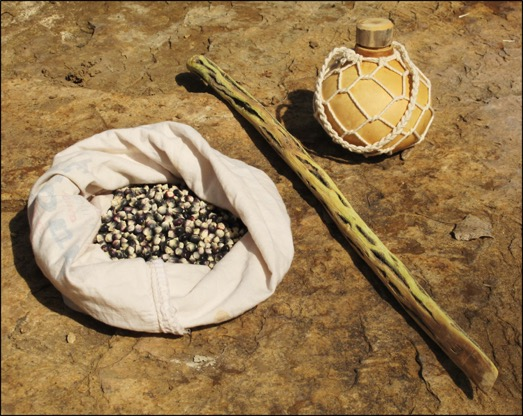
\includegraphics{./images/gifts_of_life.jpg}
\caption{A bag of seed, a digging stick, and a gourd of water; the gifts of life.}
\end{figure}

\begin{quote}
When the people emerged into this world Masau'u provided the people with three gifts---a planting stick (\emph{so'ya}) a bag of seeds and a gourd of water. He handed them a small ear of blue corn and told the people: ``Here is my life and my spirit. This is what I have to give you.''

--- A portion of a Hopi origin story
\end{quote}

To contemporary Pueblo people, corn is considered a mother because it sustains the people both physically and spiritually. Corn is also a child --- it needs constant protection and encouragement to grow to maturity. After harvest, the plants die and are laid to rest just as people are. Nourishment provided by corn in turn allows the people to care for the growing plants. The symbolic cycle of corn and people repeats over and over.

\hypertarget{a-world-of-corn}{%
\subsection{A world of corn}\label{a-world-of-corn}}

Maize was unknown outside the New World before the sixteenth century. Because of its ability to grow in diverse climates, maize spread rapidly to the rest of the world and became the staple it is today.

\begin{figure}
\centering
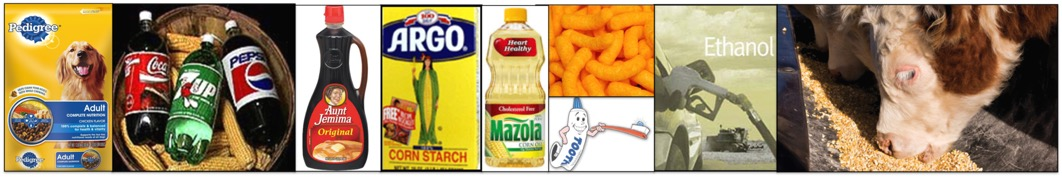
\includegraphics{./images/corn_uses.jpg}
\caption{Corn is used in thousands of every day products from cosmetics and crayons to ethanol fuel.}
\end{figure}

The success of maize worldwide can be attributed to the following:

\textbf{Adaptation} --- Contemporary varieties of maize grow in many different environmental conditions: from sea level to 11,000 feet and from 5 to 170 inches of precipitation annually.

\textbf{Variability in appearance} --- Ears and kernels display a diverse range of sizes, colors, and endosperm textures. There are thousands of varieties of corn to choose from in seed catalogs: open-pollenated, heirloom, hybrid, and even genetically modified. Variability in kernel shape, size, and color, as well as differences in ear size, demonstrates the incredible diversity in maize.

\begin{figure}
\centering
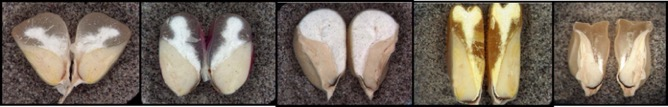
\includegraphics{./images/endosperm_types.jpg}
\caption{Kernels showing endosperm type: pop, flint, flour, dent and sweet corn (left to right). Most corn varieties can be divided into five types based on endosperm texture, or the amount of hard versus soft starch in the kernel. Each type varies in its ratio of hard (dark) to soft (white) starch and sugar. The seed embryo is located at the base of the kernel.}
\end{figure}

\textbf{Versatility} --- Products range from cereal and sweeteners to fuel. Maize may be stored as dried grain, liquid sweeteners, or alcohol. Maize can be eaten boiled, roasted, popped, or ground.

Genetic diversity is important in adapting to a wide variety of environments and conditions. Hopi farmers have at least 17 locally adapted varieties of corn. This diversity allows plants to adjust to the arid environment of the region and reduce the risk of crop failure.

\hypertarget{the-life-cycles-of-maize}{%
\section{The life cycles of maize}\label{the-life-cycles-of-maize}}

\begin{figure}
\centering
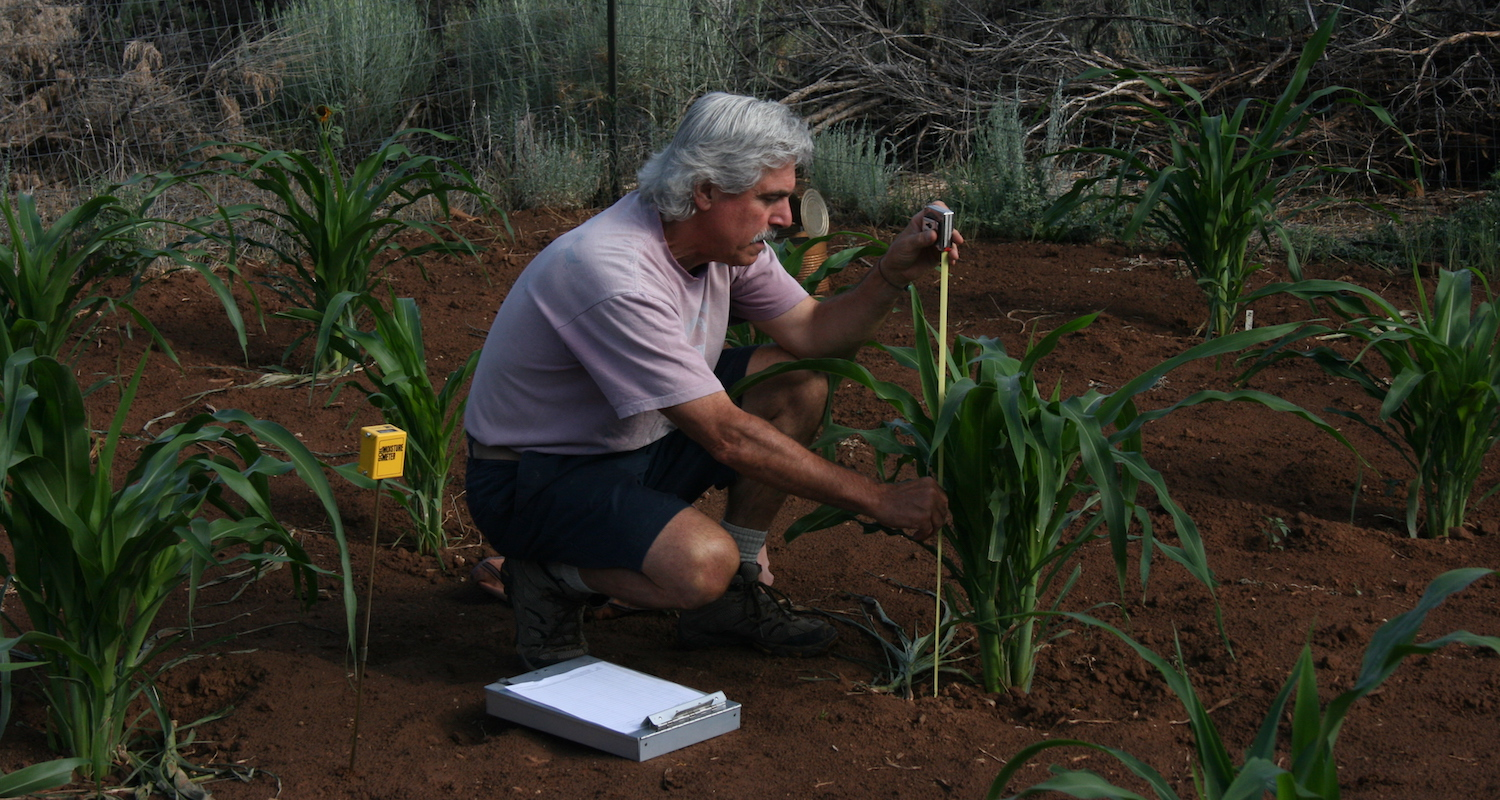
\includegraphics{./images/chapter_3_header.jpg}
\caption{Paul Ermigiotti records the growth of maize in the Check Dam Garden.}
\end{figure}

All farmers combine intimate knowledge about the crops they grow with in-field observations of how their crops are doing during the growing season. They use this information throughout the growing season when making decisions about how to care for their crops. Farmers from different cultures often have different ``ways of knowing'' about how their crops are doing.

Here, we present two ways of knowing that describe the life cycle of maize. \protect\hyperlink{the-hopi-life-cycle-of-maize}{The Hopi life cycle of maize} emphasizes the relationship between Hopi farmers and their corn that has sustained the Hopi people for generations. \protect\hyperlink{the-phenology-of-maize}{The phenology of maize} are the growth stages that scientists record to understand the life cycle of maize.

\hypertarget{the-hopi-life-cycle-of-maize}{%
\subsection{The Hopi life cycle of maize}\label{the-hopi-life-cycle-of-maize}}

All farmers use descriptions of the life cycle of their crops. The descriptions used by traditional farmers such as the Hopi reflect their traditional ecological knowledge about how their particular varieties of maize grow. The words provided in the images below are the Hopi words for the growth-stages of maize.

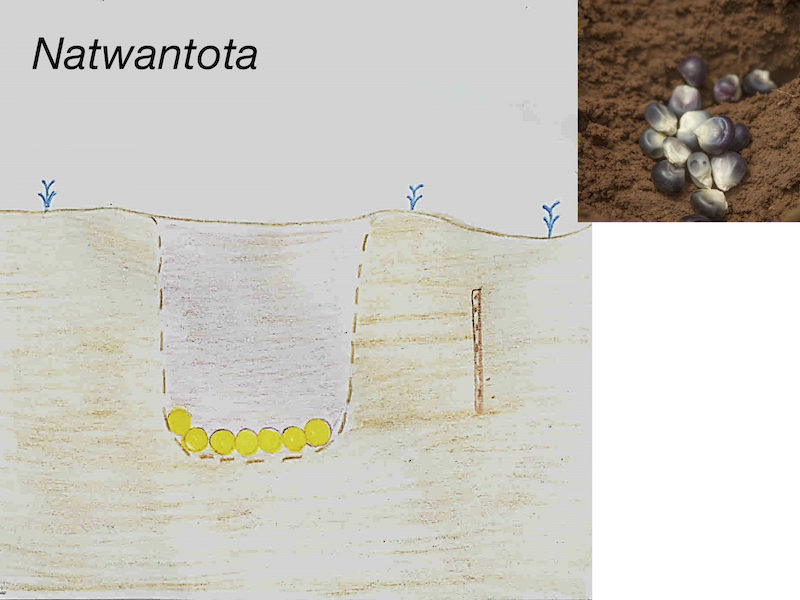
\includegraphics{./images/hopi_growth/1_nawantota.jpg}
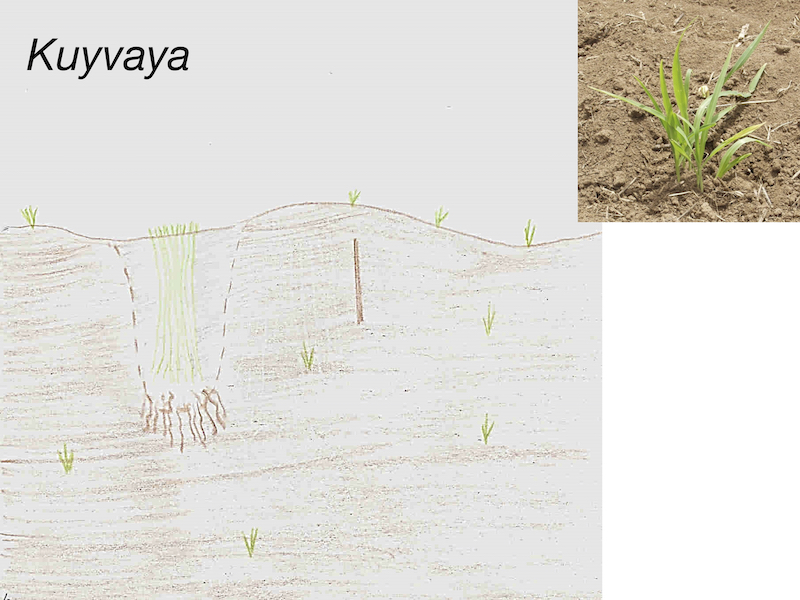
\includegraphics{./images/hopi_growth/2_kuyvaya.jpg}
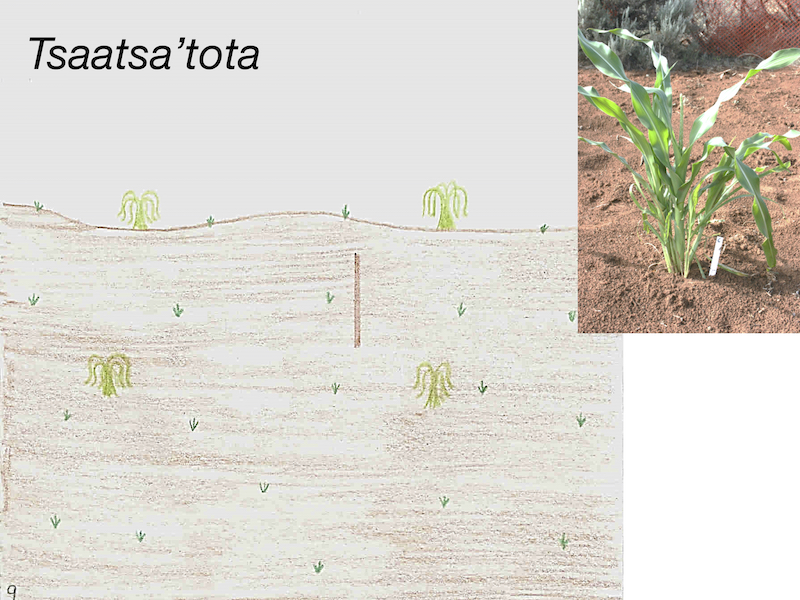
\includegraphics{./images/hopi_growth/3_tsaatsatota.jpg}
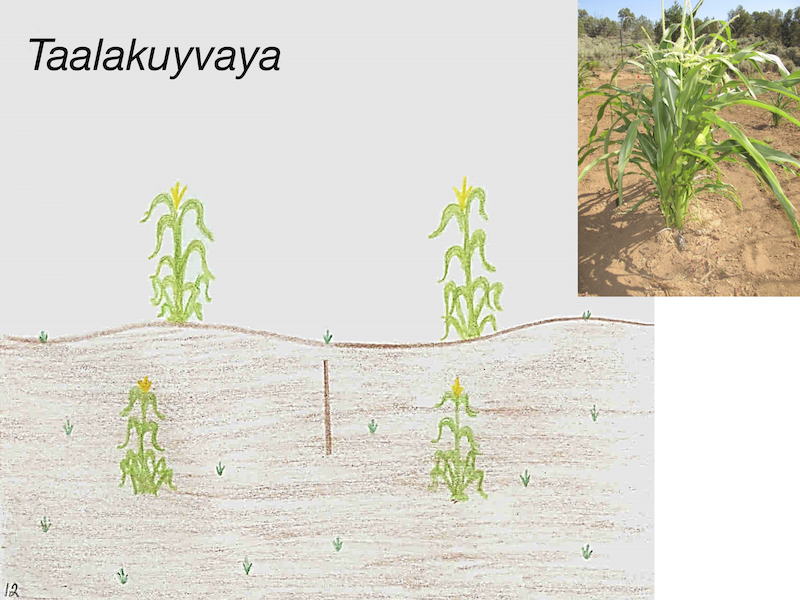
\includegraphics{./images/hopi_growth/4_taalakuyvaya.jpg}
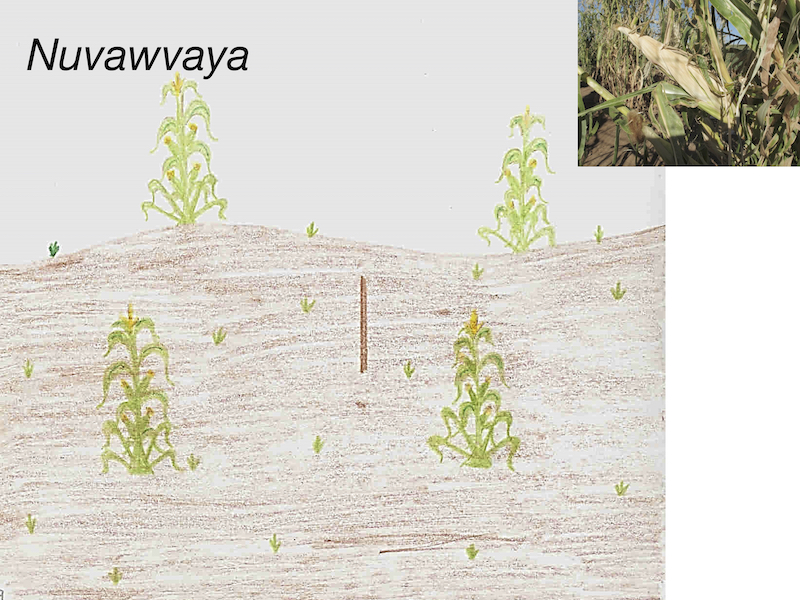
\includegraphics{./images/hopi_growth/5_nuvawvaya.jpg}
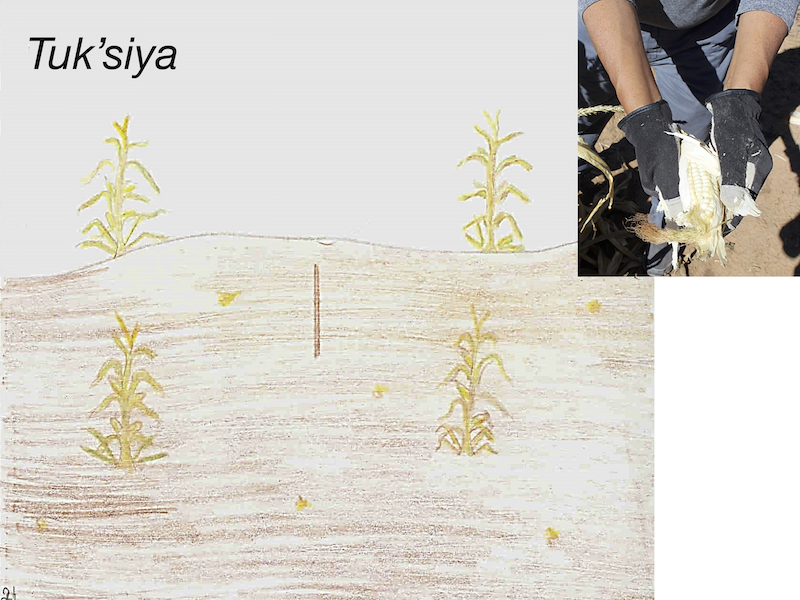
\includegraphics{./images/hopi_growth/6_tuksiya.jpg}
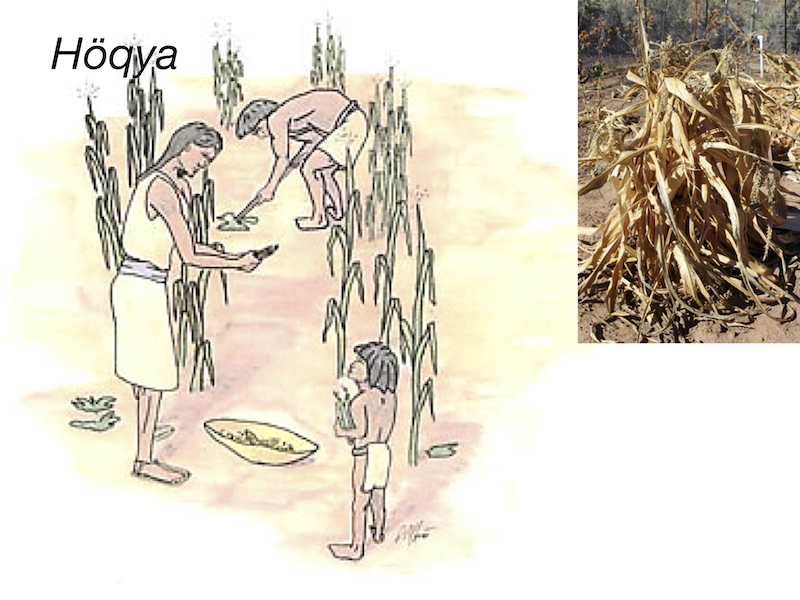
\includegraphics{./images/hopi_growth/7_hoqya.jpg}
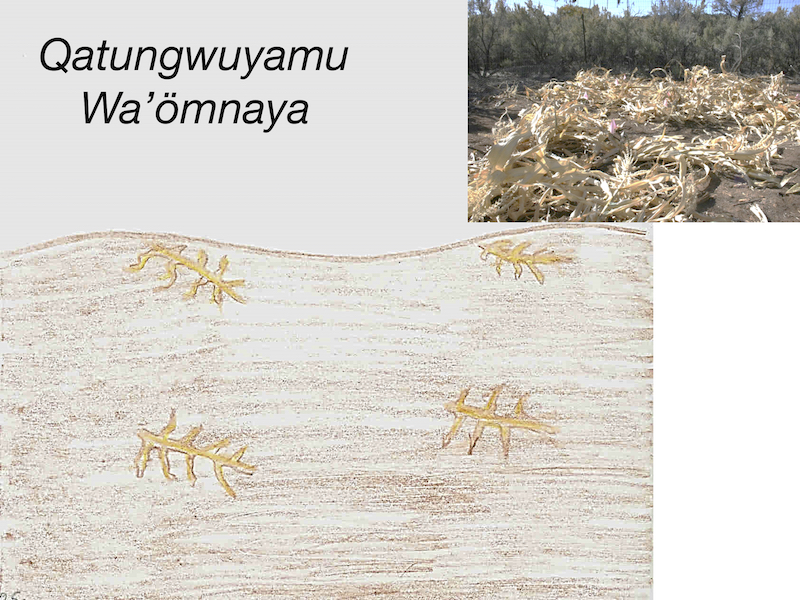
\includegraphics{./images/hopi_growth/8_qatungwuyamu_waomnaya.jpg}
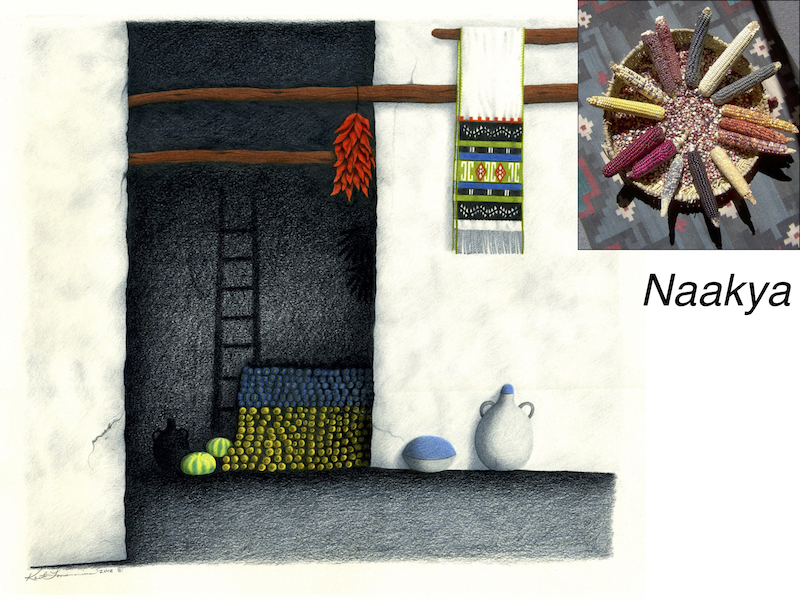
\includegraphics{./images/hopi_growth/9_naakya.jpg}

~

\hypertarget{the-phenology-of-maize}{%
\subsection{The phenology of maize}\label{the-phenology-of-maize}}

Like the Hopi, Pueblo Farming Project researchers also have desccriptions for the life cycle of maize. Pueblo Farming Project scientists use stages of maize growth from maize \emph{phenology}, or the scientific study of how plant growth and reproduction relates to the environment. The photographs below illustrate the growth stages that were recorded by Pueblo Farming Project researchers during the growing season.

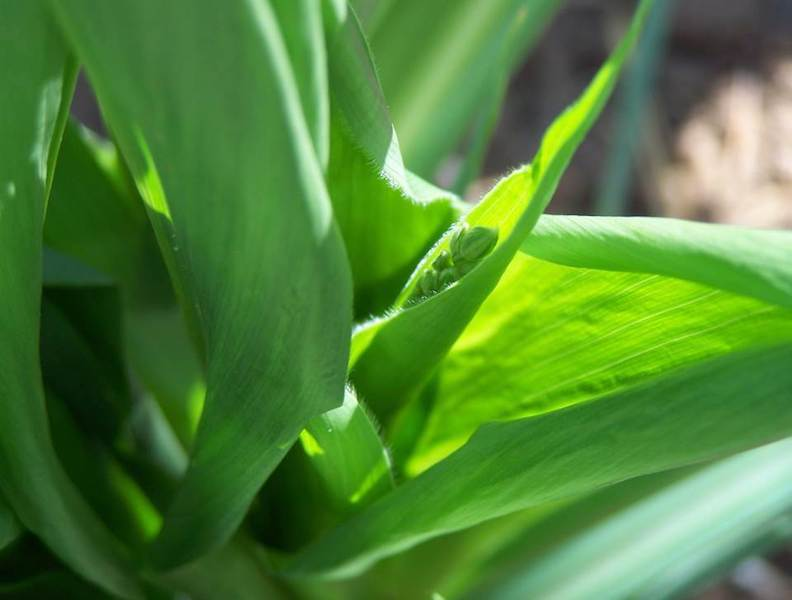
\includegraphics{./images/growth/1_early_tassel_development.jpg}
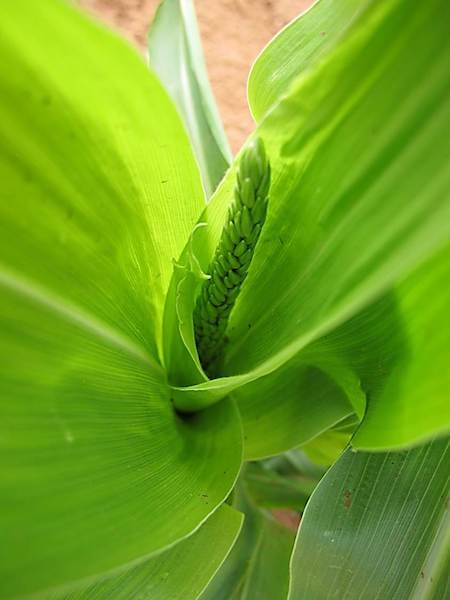
\includegraphics{./images/growth/2_early_tassel_development.jpg}
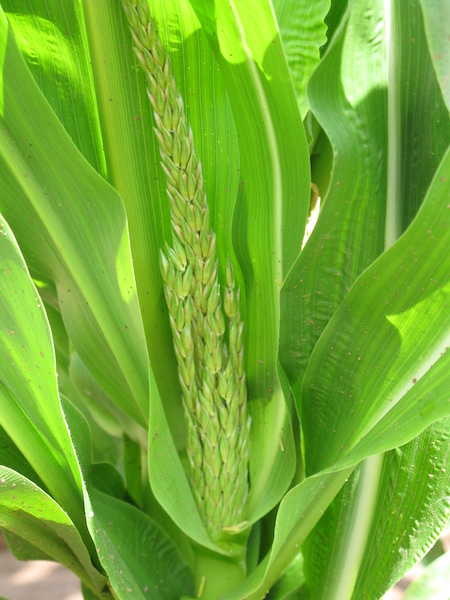
\includegraphics{./images/growth/3_tassel_development.jpg}
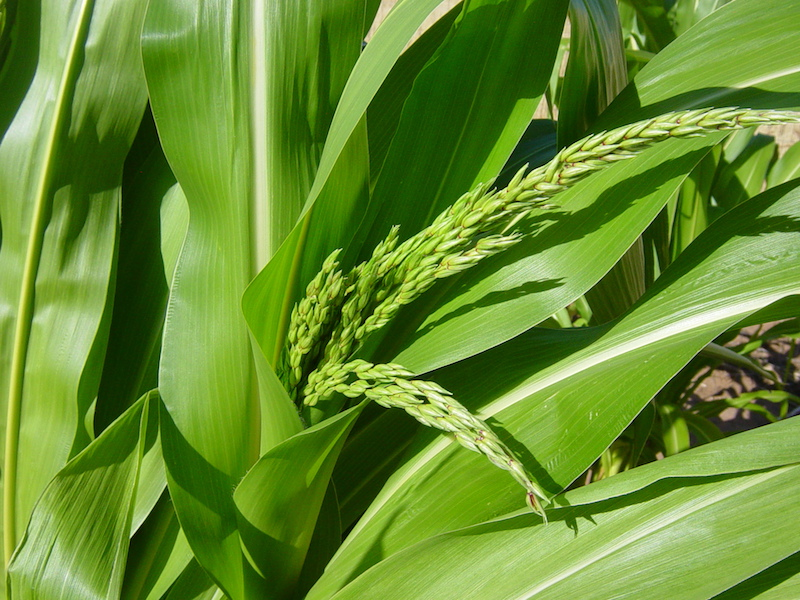
\includegraphics{./images/growth/4_tassel_development.jpg}
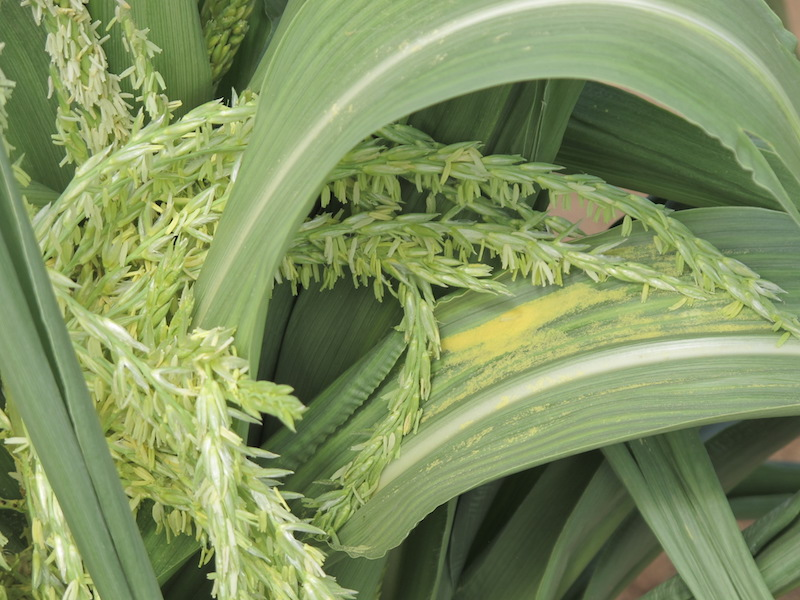
\includegraphics{./images/growth/5_tasseling.jpg}
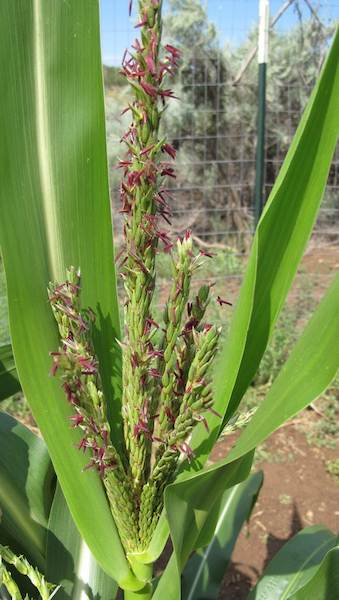
\includegraphics{./images/growth/6_tasseling.jpg}
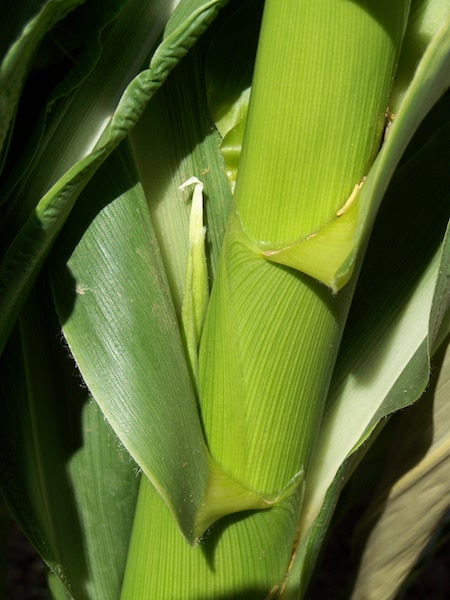
\includegraphics{./images/growth/7_silk_development.jpg}
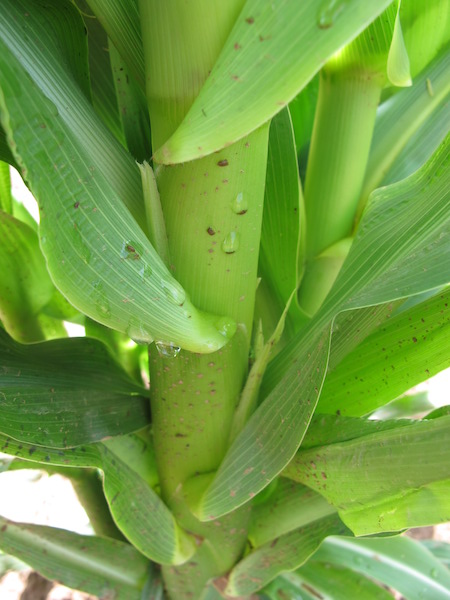
\includegraphics{./images/growth/8_silk_development.jpg}
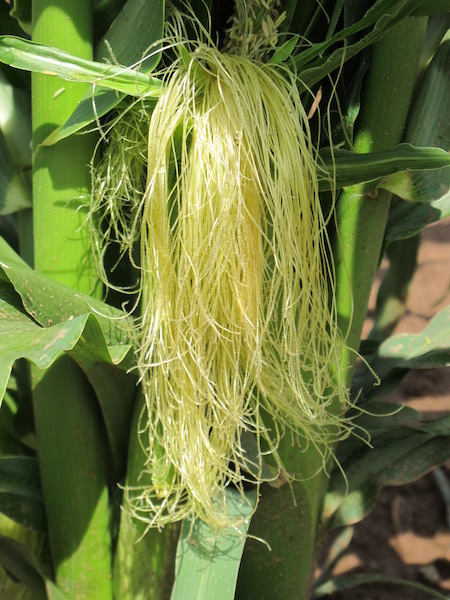
\includegraphics{./images/growth/9_silking.jpg}
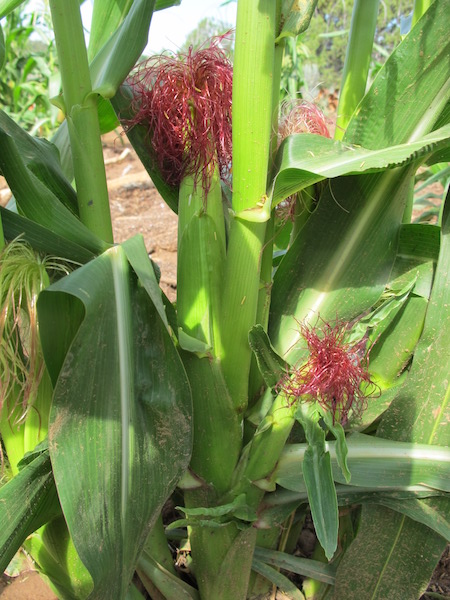
\includegraphics{./images/growth/10_silking.jpg}
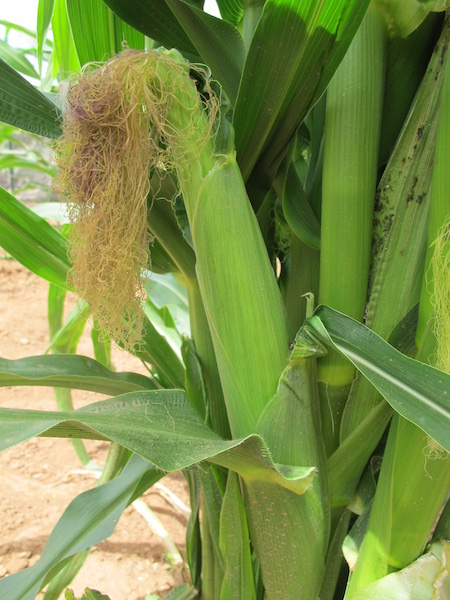
\includegraphics{./images/growth/11_ear_development.jpg}
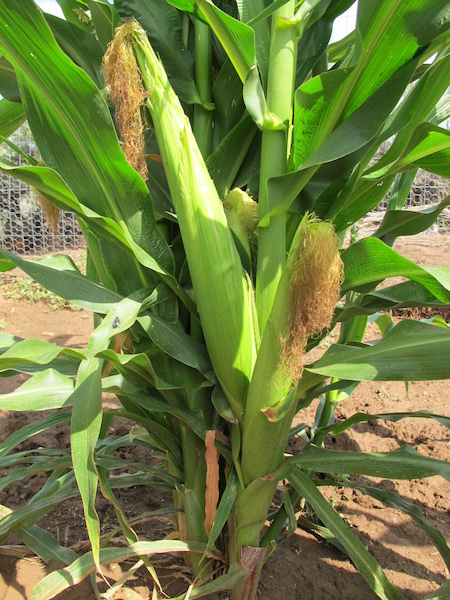
\includegraphics{./images/growth/12_ear_development.jpg}
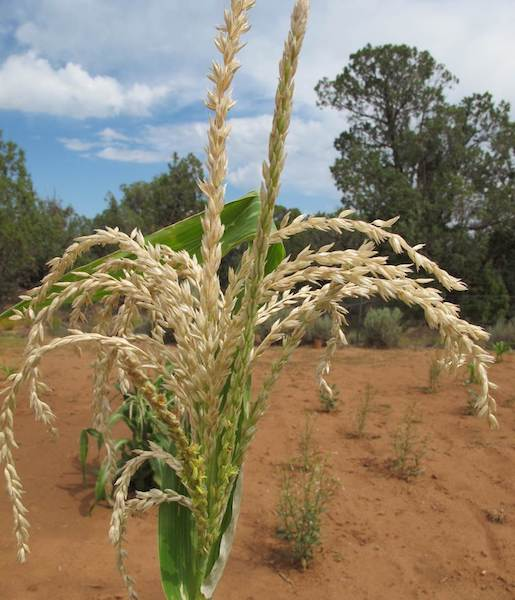
\includegraphics{./images/growth/13_maturity.jpg}

~

\hypertarget{what-maize-needs-to-flourish}{%
\section{What maize needs to flourish}\label{what-maize-needs-to-flourish}}

\begin{figure}
\centering
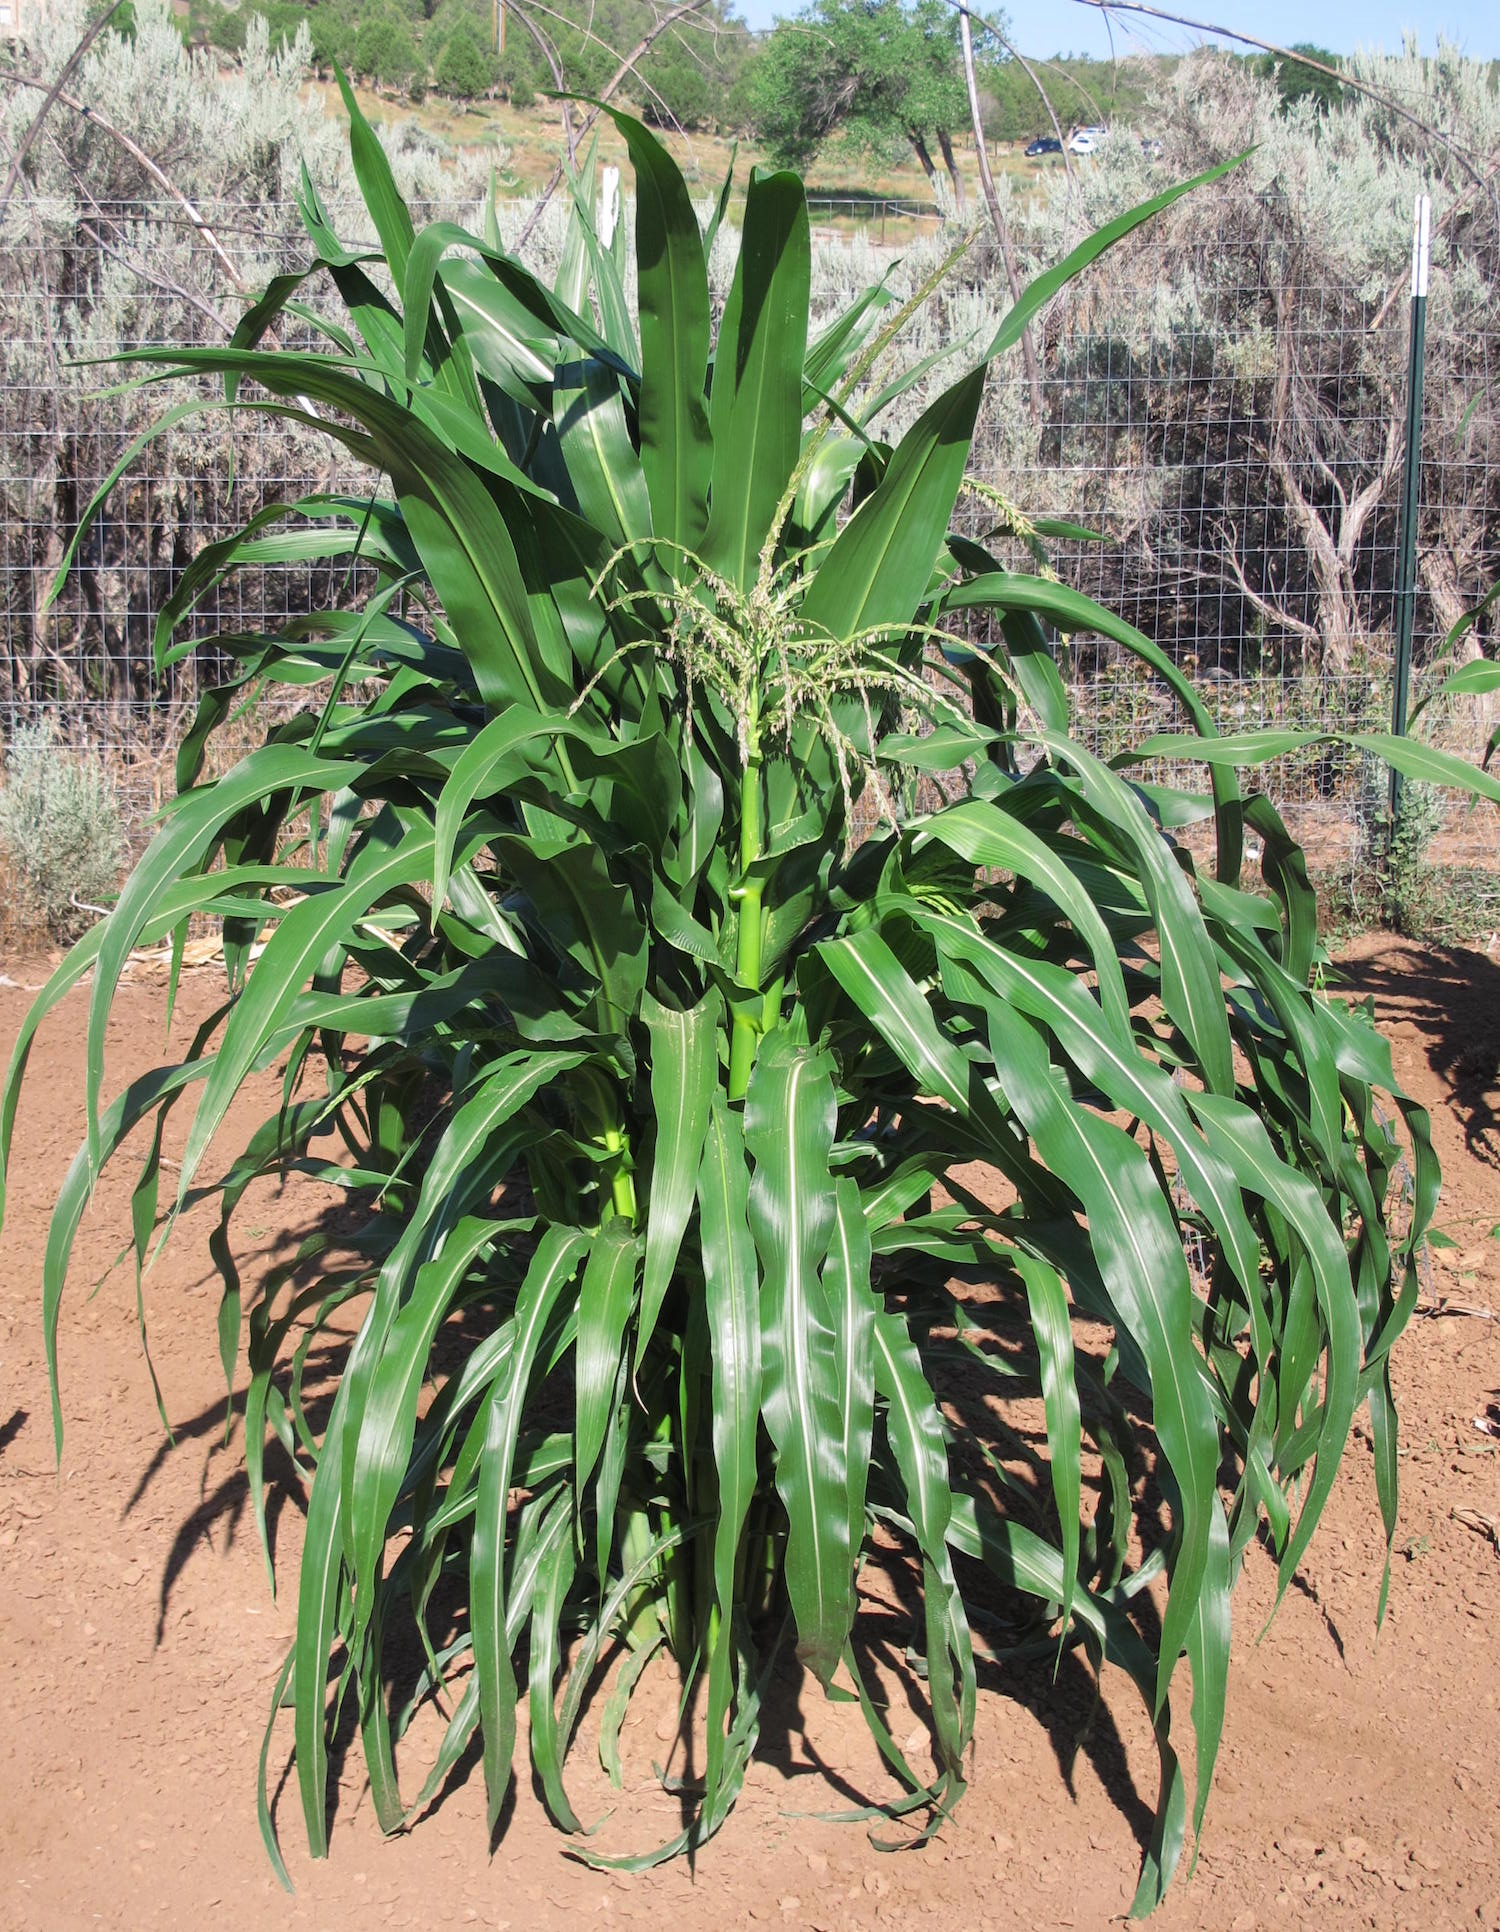
\includegraphics{./images/chapter_4_header.jpg}
\caption{A tasseling maize plant.}
\end{figure}

Maize plants, like all crops, require nutrients from the soil, water, and heat and sunlight in order to flourish. In this chapter, we explore how Pueblo maize uses each of these resources and how those resources affected the Pueblo Farming Project gardens.

\begin{figure}
\centering
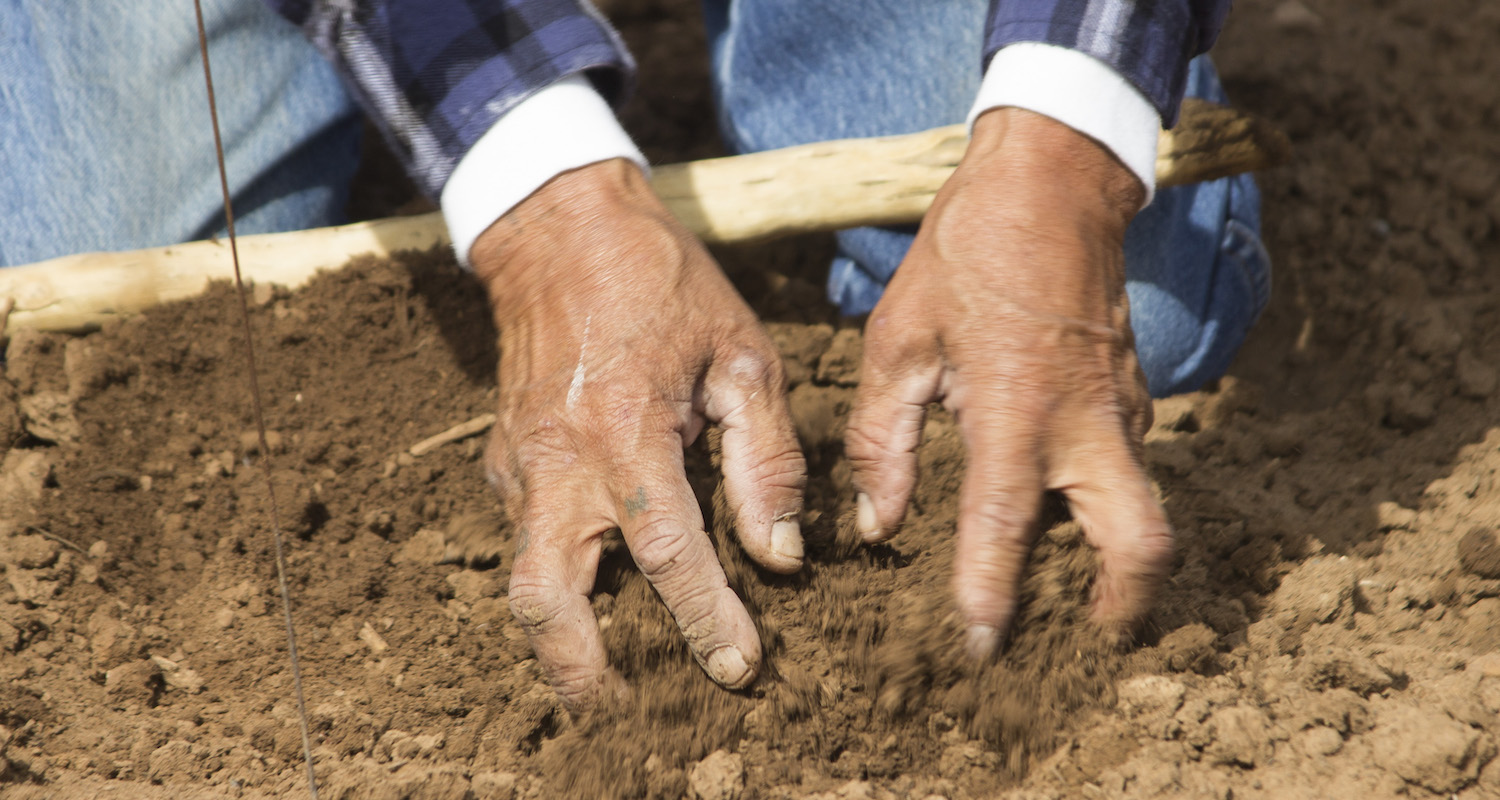
\includegraphics{./images/section_4.1_header.jpg}
\caption{A farmer places damp soil back upon the newly planted maize kernels.}
\end{figure}

\hypertarget{soils-and-water}{%
\subsection{Soils and water}\label{soils-and-water}}

\hypertarget{what-are-soils}{%
\subsubsection*{What are soils?}\label{what-are-soils}}
\addcontentsline{toc}{subsubsection}{What are soils?}

Soil is made of a combination of minerals, organic matter, and sediment. These three ingredients are combined in different amounts and travel long distances around the globe through gravity and the movements of glaciers, water, and wind. \textbf{Soils store water and nutrients that plants use to flourish.}

\hypertarget{how-does-soil-gain-water}{%
\paragraph{How does soil gain water?}\label{how-does-soil-gain-water}}
\addcontentsline{toc}{paragraph}{How does soil gain water?}

Water is delivered to the soil in two ways:

\begin{itemize}
\tightlist
\item
  \textbf{The Earth's water cycle}: precipitation in the form of rain, snow and ice. In the Southwest, the most important weather events that deliver water to the soil are winter snowstorms and summer monsoon rains.
\item
  \textbf{Water management}: Humans capture and store water from the water cycle and spread it on the soil using irrigation systems.
\end{itemize}

This video from \href{https://themonsoonproject.org/}{The Monsoon Project} describes the importance of the North American Monsoon to the Southwest.

\hypertarget{how-does-soil-lose-water}{%
\paragraph{How does soil lose water?}\label{how-does-soil-lose-water}}
\addcontentsline{toc}{paragraph}{How does soil lose water?}

Soils lose water through a process called \textbf{evapotranspiration}. This means that the sun and the wind cause soil to lose moisture through direct evaporation and through plant tissues.

Breaking this term into two parts clarifies this definition:

\begin{itemize}
\tightlist
\item
  \textbf{Transpiration} --- plants sweat out and lose water they have received from the soil
\item
  \textbf{Evaporation} --- the soil loses water due to the wind and the sun
\end{itemize}

To slow this process, farmers often use a technique called \textbf{mulching}. Mulch is:

\begin{itemize}
\tightlist
\item
  A material that is spread over a planting area to protect the soil from the effects of the wind and the sun.
\item
  A layer of insulation that traps moisture and shades the soil, which slows evaporation.
\item
  Carbon-based materials such as straw or dry grass clippings.
\end{itemize}

Pueblo farmers, such as the Hopi, use dust and sand as a mulch; they cover the moist soil that holds their seeds with a thick layer of sand and dust.

\hypertarget{why-do-some-farmers-apply-irrigation-water-to-their-soil}{%
\paragraph{Why do some farmers apply irrigation water to their soil?}\label{why-do-some-farmers-apply-irrigation-water-to-their-soil}}
\addcontentsline{toc}{paragraph}{Why do some farmers apply irrigation water to their soil?}

Some farmers irrigate because:

\begin{itemize}
\tightlist
\item
  They are replacing the water that their plants and soils have lost due to evapotranspiration.
\item
  Some plants require more water than the environment has to offer; the farmers apply irrigation water to make up for water that does not arrive in the form of rain and snow.
\end{itemize}

Some modern farmers do not apply irrigation water to their soil:

\begin{itemize}
\tightlist
\item
  Hopi farmers who have vast direct-precipitation corn fields.
\item
  Farmers in the Western states who have large direct-precipitation crop farms.
\end{itemize}

Many Hopi farmers and other farmers in the Southwest do not use irrigation systems; the keys to their success are understanding weather patterns, caring for their soil, planting drought-resilient seeds, and having faith in natural cycles.

\begin{quote}
\textbf{\emph{``Dry-farming in the high desert \ldots{} relying only on precipitation and runoff water, requires an almost miraculous level of faith and is sustained by hard work, prayer, and an attitude of deep humility.''}}

--- Wall and Masayesva 2004:436
\end{quote}

\hypertarget{how-do-direct-precipitation-farmers-decide-where-to-place-their-gardens-and-fields-why-is-this-decision-so-important}{%
\paragraph{How do direct-precipitation farmers decide where to place their gardens and fields? Why is this decision so important?}\label{how-do-direct-precipitation-farmers-decide-where-to-place-their-gardens-and-fields-why-is-this-decision-so-important}}
\addcontentsline{toc}{paragraph}{How do direct-precipitation farmers decide where to place their gardens and fields? Why is this decision so important?}

Choosing the location of a garden is called \emph{site selection}. It is important to direct-precipitation farmers because the chosen site must be able to capture and hold water delivered by the water cycle, making it drought resilient.

\textbf{These are features that Hopi farmers of today look for---and that ancestral Pueblo farmers probably also looked for---when searching for a drought-resilient site.}:

\begin{itemize}
\tightlist
\item
  \textbf{Geography}: Rainfall and snowmelt that drains off of a mesa or cliff will collect and flow into drainages, washes, arroyos, and canyons. Where these features become less narrow and widen into sandy slopes, Pueblo farmers expect water and good soil to collect because it is washed down with the floodwaters. This mouth or opening is also a place where they traditionally built \textbf{check dams}---rows of low rock walls to slow down the movement of runoff water.
\item
  \textbf{Garden slope}: North-facing slopes have less direct exposure to sunlight and lower soil temperature, and therefore less water is lost to evaporation.
\item
  \textbf{Indicator plants}: The appearance of certain plants in early spring give information, or \emph{indicate}, to Hopi and other direct-precipitation farmers about the best locations for a garden/field, how deep to plant and how much space to leave between plants. Farmers combine these indications with practice, experience, and knowledge of the land. Some examples of plants that indicate these conditions are:
\end{itemize}

CONDITION

INDICATOR PLANT

Good soil moisture

Rabbitbrush
Four-wing saltbrush
Mormon tea
Rice grass
Snakeweed

Deep, well-drained soil

Rabbitbrush
Oak trees

\begin{itemize}
\tightlist
\item
  \textbf{Soil moisture depth}: deep, soft soils allow natural reservoirs of water to collect and be held deep in the soil.
\item
  \textbf{Soil color}: darker colors often mean higher amounts of decomposed organic matter and nutrients in the soil. In the Southwest, this means dark red-brown.
\item
  \textbf{Large, open planting area}: the area must be large enough that clumps of seeds can be planted with wide spaces between them (2--3 adult paces/steps or 4--6 feet between clumps.) This spacing allows little soil-moisture reservoirs to be created between clumps, providing long-term moisture.
\end{itemize}

\textbf{Soil moisture is especially important to maize growth at planting (for germination), at tasseling/silking (for best chances at pollination), and during grain fill (to get ears completely covered with kernels).}

\hypertarget{drought}{%
\subsubsection*{Drought}\label{drought}}
\addcontentsline{toc}{subsubsection}{Drought}

\textbf{When a normal amount of snow and rain does not arrive, this is called a \emph{drought}.}

\hypertarget{how-do-pueblo-farmers-respond-to-drought}{%
\paragraph{How do Pueblo farmers respond to drought?}\label{how-do-pueblo-farmers-respond-to-drought}}
\addcontentsline{toc}{paragraph}{How do Pueblo farmers respond to drought?}

The Hopi use the agricultural knowledge gained through their ancestral direct-precipitation farming practices. They want to ensure their crops will continue to be drought-resilient into the future. To survive drought, direct-precipitation farmers must know a lot about their soil and their seeds. Ancestral Pueblo farmers might have responded to drought by:

\begin{itemize}
\tightlist
\item
  anticipating the possibility that it could arrive any year and preparing for it by saving seeds from plants that can survive drought.
\item
  using the site-selection factors listed above to decide whether or not a site would be drought-resilient.
\item
  meeting these site requirements by planting in multiple locations.
\item
  using clumps of plants, twigs, or brush at the edge of the planting area or placing small upright stone slabs around seedlings as a windbreak to decrease evapotranspiration.
\item
  covering holes that contain seeds with loose topsoil to act as a \emph{dust mulch}.
\end{itemize}

\hypertarget{do-other-direct-precipitation-farmers-use-any-of-these-same-practices}{%
\paragraph{Do other direct-precipitation farmers use any of these same practices?}\label{do-other-direct-precipitation-farmers-use-any-of-these-same-practices}}
\addcontentsline{toc}{paragraph}{Do other direct-precipitation farmers use any of these same practices?}

Yes, though some farmers emphasize knowing the soil through soil testing:

\begin{itemize}
\tightlist
\item
  First, farmers learn what is in their soil to determine what kind of soil they have.
\item
  Second, farmers find out how much water their soil can hold. If the soil receives more water than it can hold, much of the extra water will drain away. Water that is wasted in this way is called \textbf{runoff}; it leads to \textbf{erosion}, when soil is carried away by the runoff.
\end{itemize}

\hypertarget{soils-in-the-pfp-gardens}{%
\subsubsection*{Soils in the PFP gardens}\label{soils-in-the-pfp-gardens}}
\addcontentsline{toc}{subsubsection}{Soils in the PFP gardens}

Pueblo Farming Project researchers used data from the USDA and local soil analysis to characterize the soils in the gardens on Crow Canyon's campus in southwestern Colorado. The map below displays the soils on Crow Canyon's campus. Click a soil to learn more information about it!


\includegraphics{images/unnamed-chunk-2-1.pdf}

\hypertarget{heat-and-sunlight}{%
\subsection{Heat and sunlight}\label{heat-and-sunlight}}

\begin{figure}
\centering
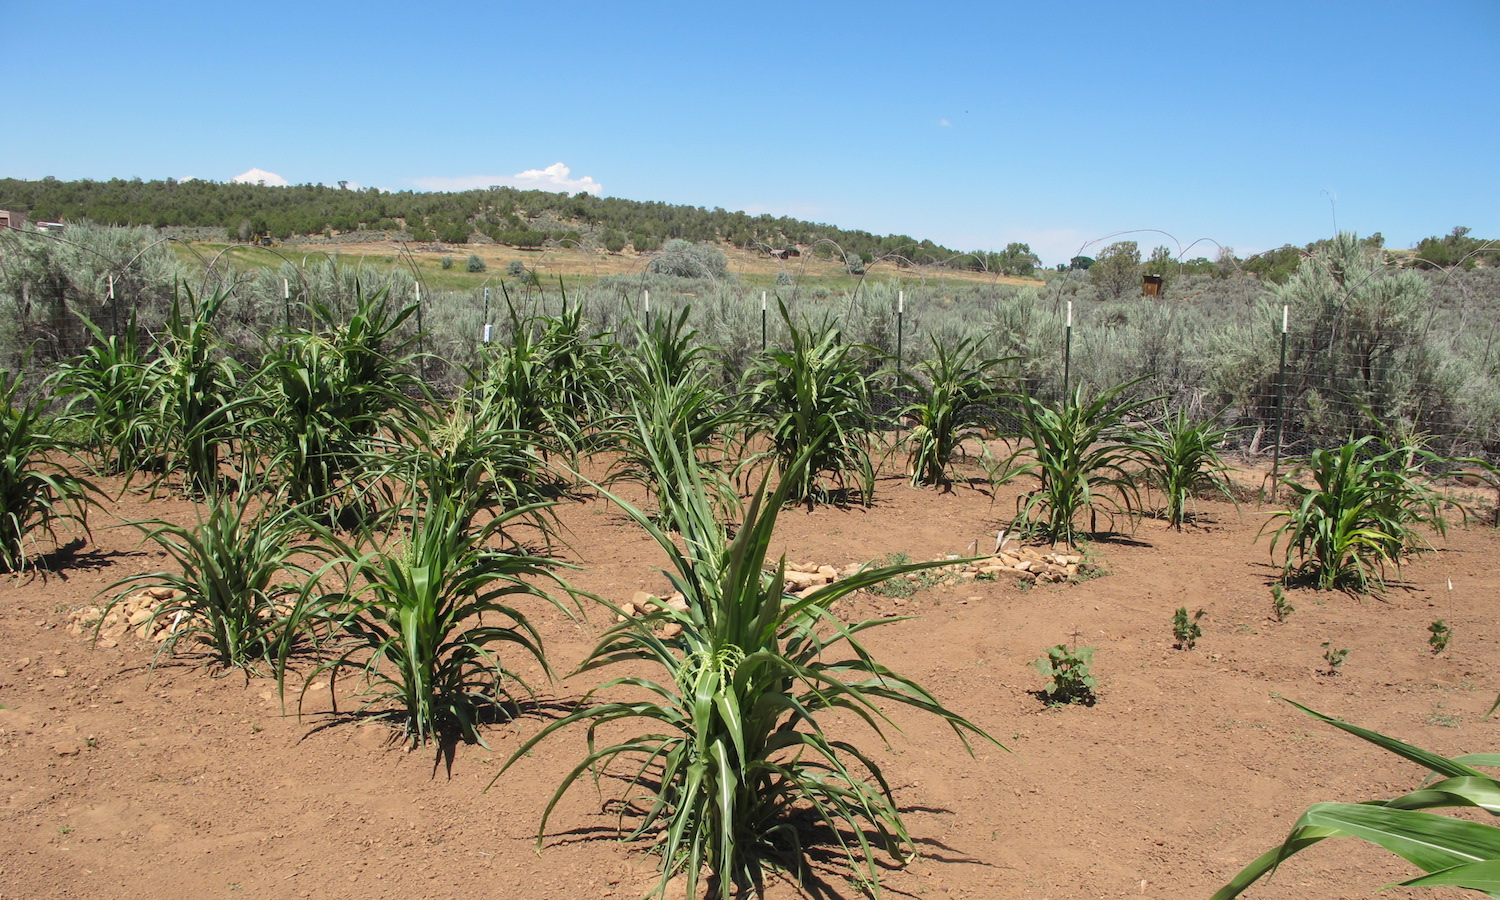
\includegraphics{./images/section_4.3_header.jpg}
\caption{The Check Dam Garden on the Crow Canyon Archaeological Center campus.}
\end{figure}

All plants require thermal energy---in the form of heat and sunlight---to perform \textbf{photosynthesis} and flourish. Photosynthesis is a process used by plants to make a sugary food that fuels their growth. Plants absorb the energy of the sun through their leaves, combine it with water and carbon dioxide, and make a sugar called glucose. \textbf{Fun Fact: The waste product that this process creates is oxygen!} Farmers in ancient times adapted their corn to the amount of heat and sunlight available in the regions in which they lived, and farmers today do the same.

But how much heat does a plant need, and how do we know how much it gets? Plant researchers use a measure of accumulated heat called a \textbf{growing degree day (GDD)} to estimate the amount of heat that plants may use for photosynthesis.

The equation for daily GDD for maize is:
\[ GDD=\frac{T_{MAX} + T_{MIN}}{2}-T_{BASE} \]
where \(T_{MAX}\) is the maximum daily temperature, \(T_{MIN}\) is the minimum daily temperature and \(T_{BASE}\) is the temperature below which plant growth ceases, which we take to be 10°C (\textasciitilde50ºF) for maize.

Here we use a series of corrections to the equation typically applied for calculating maize GDD, which down-corrects \(T_{MAX}\) and \(T_{MIN}\) to an upper threshold (\(T_{UT}\), here 30°C or 86ºF) above which corn growth does not appreciably increase, and up-corrects \(T_{MAX}\) and \(T_{MIN}\) if they fall below \(T_{BASE}\) (here 10°C or 50ºF). To summarize:
\[
\text{if} \quad T_{MAX}>T_{UT}, \quad T_{MAX}=T_{UT}\\
\text{if} \quad T_{MIN}>T_{UT}, \quad T_{MIN}=T_{UT}\\
\text{if} \quad T_{MAX}<T_{BASE}, \quad T_{MAX}=T_{BASE}\\
\text{if} \quad T_{MIN}<T_{BASE}, \quad T_{MIN}=T_{BASE}
\]

Growing degree day amounts calculated in Celsius are different from those calculated in Fahrenheit. Growing degree days can be converted from Celsius heat units to Fahrenheit heat units by multiplying by a factor of 1.8. For example, 1000 Celsius GDDs are equal to 1800 Fahrenheit GDDs.

\hypertarget{weather-in-cortez}{%
\subsubsection*{Weather in Cortez}\label{weather-in-cortez}}
\addcontentsline{toc}{subsubsection}{Weather in Cortez}

\begin{figure}
\centering
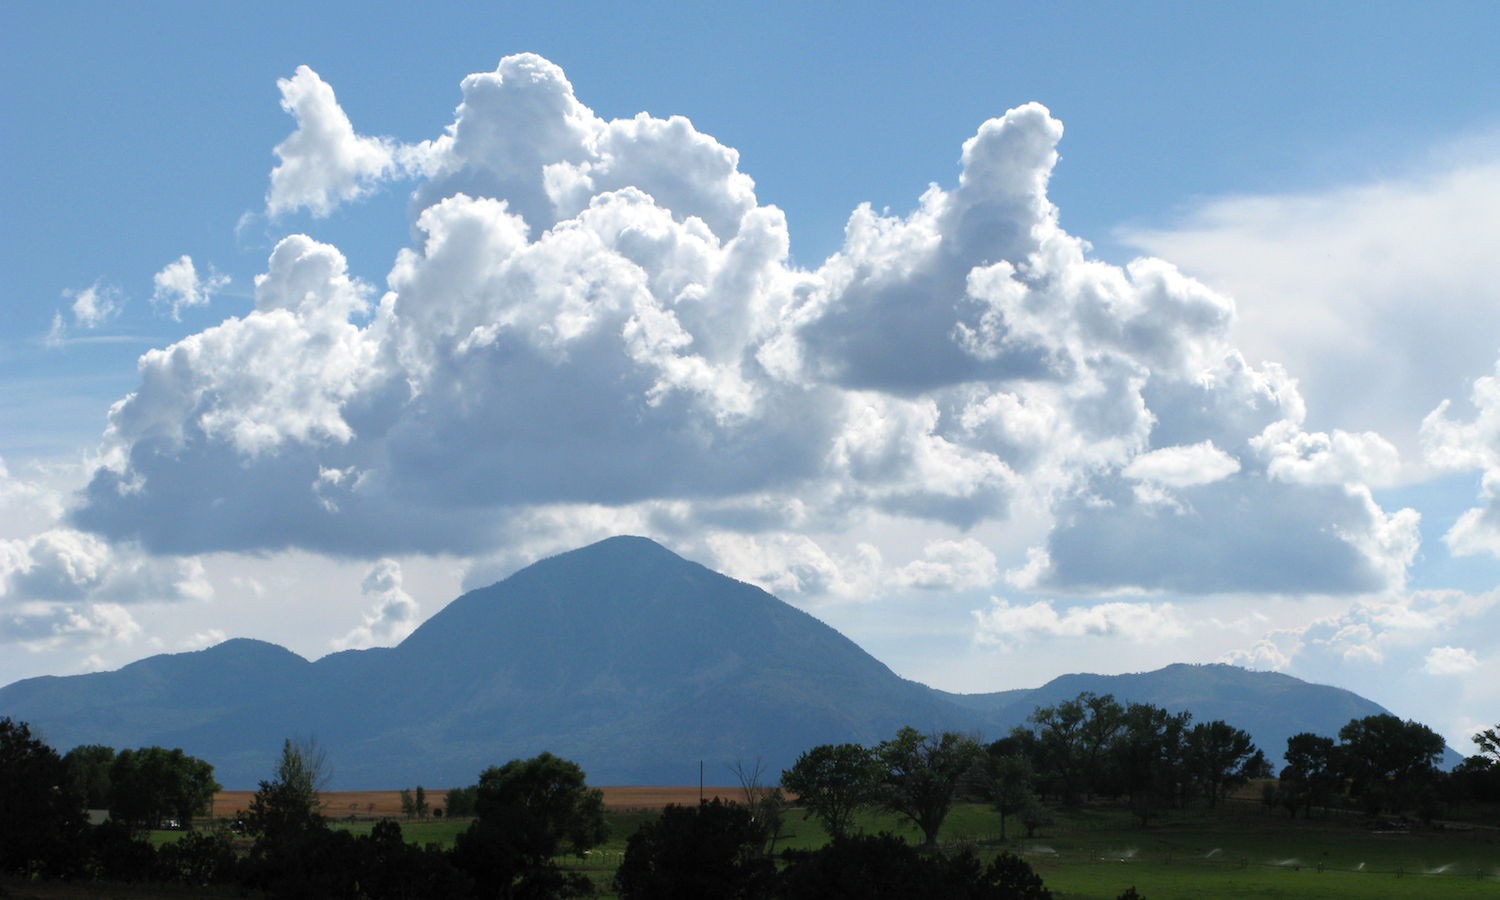
\includegraphics{./images/section_4.2_header.jpg}
\caption{Rain clouds gather over Ute Mountain in southwestern Colorado.}
\end{figure}

Plants combine water and nutrients from the soil with heat and energy from the Sun to flourish. Pueblo Farming Project researchers estimated the amount of water and accumulated heat available to the maize in the Pueblo Farming Project gardens using weather data gathered by the US National Oceanic and Atmospheric Administration (NOAA) as part of the US Historical Climatology Network (USHCN). Temperature and precipitation data from a weather station in Cortez were used to measure the response of the Pueblo Farming Project gardens to local weather; we also installed a weather station on Crow Canyon's campus as well as temperature monitors in each garden. The graphs below show 2009 to 2018 data for the Pueblo Farming Project gardens. The top graph shows minimum and maximum daily temperatures and daily growing degree days, and the lower graph shows daily precipitation events. \textbf{These graphs are interactive!} Highlight a region of the graph in order to explore the weather. Hover over a graph to see the recorded weather at the Cortez weather station.

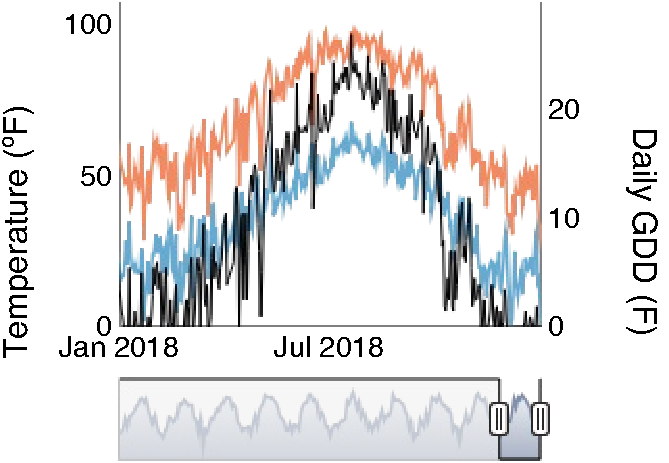
\includegraphics[width=1\linewidth]{images/unnamed-chunk-3-1}
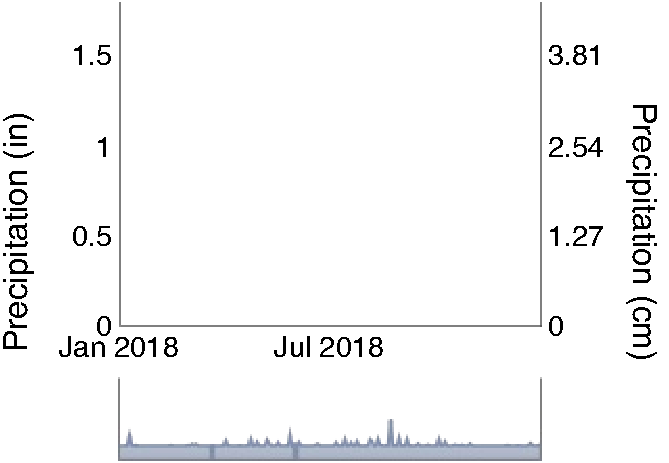
\includegraphics[width=1\linewidth]{images/unnamed-chunk-3-2}

\hypertarget{the-pfp-field-experiments}{%
\section{The PFP field experiments}\label{the-pfp-field-experiments}}

\begin{figure}
\centering
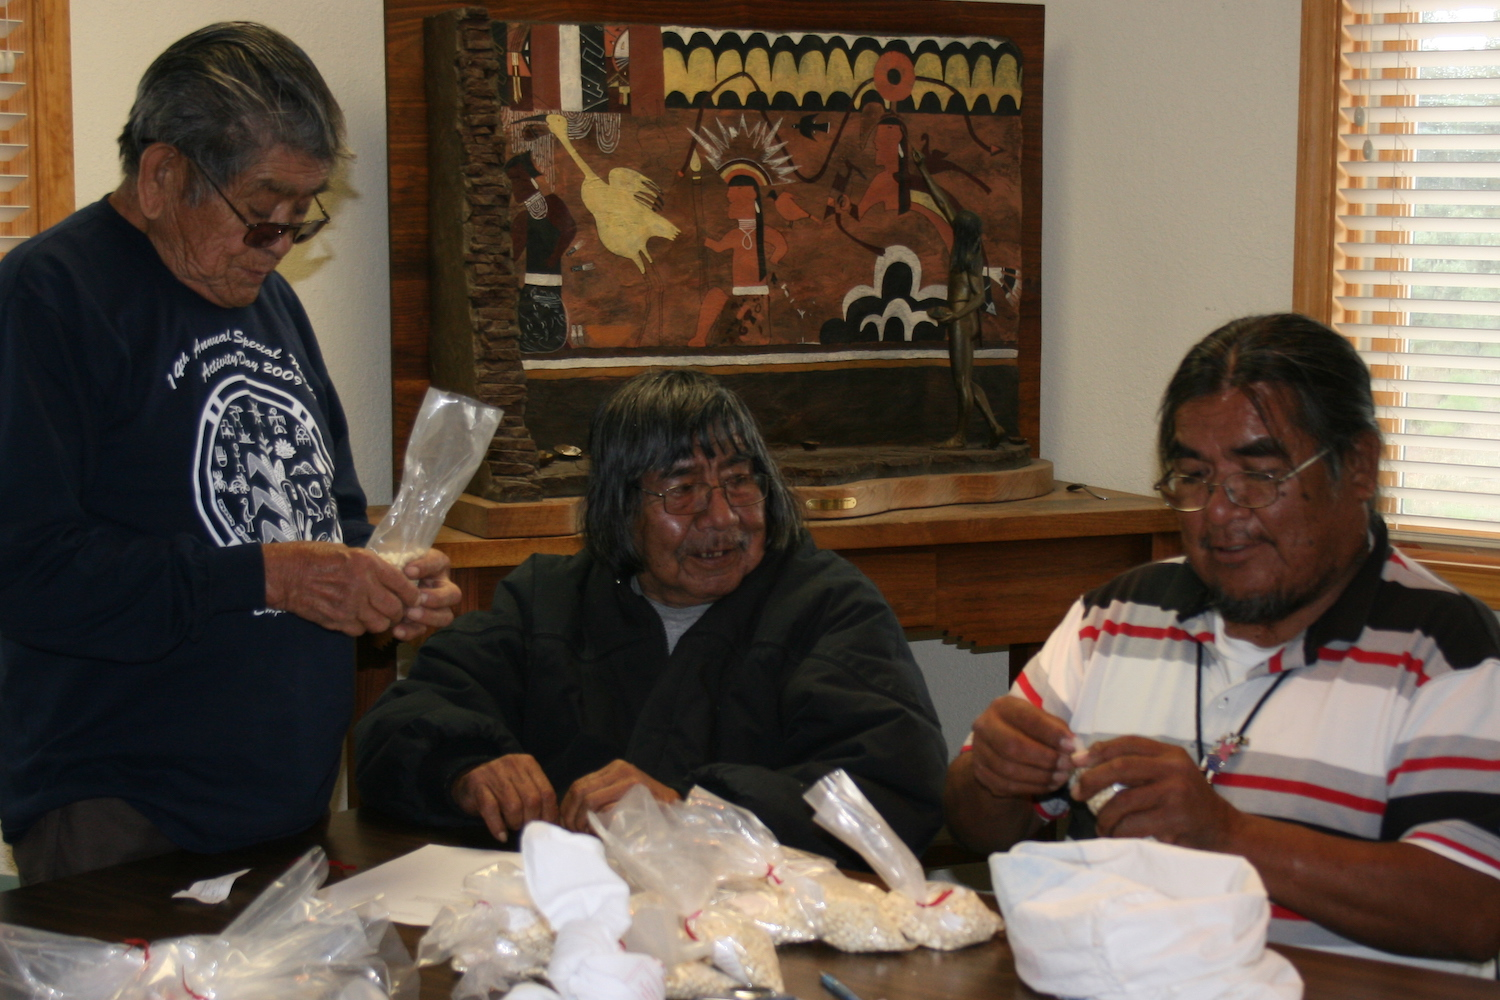
\includegraphics{./images/chapter_5_header.jpg}
\caption{Examining the results of the previous year's yield.}
\end{figure}

\hypertarget{procedure}{%
\subsection{Procedure}\label{procedure}}

\hypertarget{planting}{%
\subsubsection*{Planting}\label{planting}}
\addcontentsline{toc}{subsubsection}{Planting}

\begin{figure}
\centering
\includegraphics{./images/chapter_6_soya.jpg}
\caption{Using a traditional Hopi planting stick, or \emph{so'ya}.}
\end{figure}

The primary tool for planting is a planting stick or, in the Hopi language, a \emph{so'ya}. Traditionally a \emph{so'ya} is made from greasewood (\emph{Sarcobatus vermicalatus}), but some planting sticks today are made from a length of metal pipe with a narrow blade welded to one end.

Planting begins by using your foot to scrape away the upper layer of loose, dry dirt. This exposes the top of the underlying hard-packed soil. About a square foot area is cleared. The planter gets down on one knee and grabs the \emph{so'ya} with one hand low and one hand higher up on the tool. A narrow hole is dug using a pulling motion toward the planter. Typically, the hole is dug to a depth of about 8 to 10 inches or to the depth where good soil moisture is encountered. The hole is dug deeper if the soil is drier and shallower if the soil is moist. This soil moisture is critical for plant germination and for the plant to be able to grow until there is more precipitation, which might not occur until many weeks after planting.

Hopi farmers plant corn in clumps. 10--20 seeds are deposited into the hole. The excavated earth is put back gently into the hole in the order it was removed with the moist soil covering the seeds on the bottom and the drier soil on top. The loose dry dirt is on the top, but a small basin is created on the surface to collect any precipitation that falls and to create a dust mulch that reduces evaporation.

The farmer stands and takes two or three steps to measure where the next clump of corn will be planted. Because the soils in the PFP gardens hold a bit more moisture than those soils near the Hopi mesas, the PFP clumps are typically spaced about 1.5--1.75 meters apart rather than the three-meter spacing typically used at Hopi. The wide spacing of the planted clumps reduces competition for valuable sub-surface moisture.

Flick through these slides to see how planting is done the Hopi way! The descriptions are based on \emph{Notes On Hopi Economic Life} by Earnest Beaglehole, 1937.

\includegraphics{./images/planting/1_planting.jpg}
\includegraphics{./images/planting/2_planting.jpg}
\includegraphics{./images/planting/3_planting.jpg}
\includegraphics{./images/planting/4_planting.jpg}
\includegraphics{./images/planting/5_planting.jpg}
\includegraphics{./images/planting/6_planting.jpg}
\includegraphics{./images/planting/7_planting.jpg}
\includegraphics{./images/planting/8_planting.jpg}
\includegraphics{./images/planting/9_planting.jpg}

~

\hypertarget{monitoring}{%
\subsubsection*{Monitoring}\label{monitoring}}
\addcontentsline{toc}{subsubsection}{Monitoring}

\begin{figure}
\centering
\includegraphics{./images/chapter_3_header.jpg}
\caption{Paul Ermigiotti records the growth of maize in the Check Dam Garden.}
\end{figure}

The procedures for monitoring Pueblo Farming Project gardens were based on those developed by Benjamin Bellorado in an experimental gardening study that he developed for the Animas-LaPlata archaeological project and for his MA thesis at Northern Arizona University. For the majority of the Pueblo Farming Project these procedures were implemented by Paul Ermigiotti and staff and volunteers who assisted him.

Monitoring was conducted each week. The primary objectives were to record growth stages, to document damage by pests, and to make other observations about the condition of the gardens. The data were recorded on paper forms in the field and later put into a database.

The data collected each week on growth stages includes the following:

\begin{itemize}
\tightlist
\item
  \textbf{Height} --- The height of the tallest plant in each clump was recorded to the nearest 5 cm.
\item
  \textbf{Early Tassel Development} --- Early tassel development was recorded when it occurred on any plant in a clump. Early tassel development is defined as the time when the tassel bud starts to emerge from the central enclosing leaves at the top of the stalk to the time the tassel spike begins to branch.
\item
  \textbf{Tassel Development} --- Tassel development was recorded when it occurred on any plant in a clump. Tassel development begins when the tassel emerges from the central cluster of leaves and begins to branch. This stage ends when the anthers (male flowers) emerge from the glumes of the tassel and the pollen begins to shed.
\item
  \textbf{Tasseling} --- The period of tasseling was recorded when it occurred on any plant in a clump. The tasseling period is when the apex inflorescences (a group of flowers) begin to open. The anthers (male flowers) emerge and begin to shed pollen. At this stage the stalk has produced all its leaves, and the plant has reached full height.
\item
  \textbf{Silk Development} --- Silk development was recorded when it occurred on any plant in a clump. Silk development is when ear shoots become visible in the nodes (between the leaf and stalk) until the silks have fully emerged and are ready to receive pollen.
\item
  \textbf{Silking} --- Silk development was recorded when it occurred on any plant in a clump. Silking is when the silk has emerged from the husk surrounding the developing cob and is capable of receiving pollen. A single silk will deliver pollen and develop into individual kernel. Once the silks have begun to dry and shrivel, this growth stage has ended.
\item
  \textbf{Ear Development} --- Ear development was recorded when it occurred on any plant in a clump. Ear development begins once the silks have dried out, shriveled, and are no longer accepting pollen and continues until the kernels mature and the ear is ready to harvest. A hard frost (below 28ºF.) will prematurely end ear development.
\end{itemize}

\hypertarget{harvesting}{%
\subsubsection*{Harvesting}\label{harvesting}}
\addcontentsline{toc}{subsubsection}{Harvesting}

\begin{figure}
\centering
\includegraphics{./images/chapter_5_harvest.jpg}
\caption{Harvesting maize.}
\end{figure}

The harvest and yield data entry for the Pueblo Farming Project is a three-step process that includes collecting the corn from the field, weighing the ears just after harvest, and, when they have dried completely, weighing the ears again to record the dry-kernel weight for each ear.

On harvest day, typically in mid-October after the ears have sufficiently ripened on the stalk, the farmers approach the garden with anticipation. All of the ears from each stalk in a clump are shucked, the silk is removed, and the ears are recorded and tagged according to the clump, stalk, and ear. After the ears are collected from a clump the stalks are bent over at the base and laid to rest on the ground. This laying to rest of the stalks is part of the life process that cycles through birth, maturation, and death. The stalks left in the garden also help with the spacing in the next year's planting. Planting between the stalks ensures that seeds are not planted in the same place two years in a row.

\begin{figure}
\centering
\includegraphics{./images/harvesting.jpg}
\caption{Harvesting maize and recording its attributes.}
\end{figure}

After harvest the ears are weighed to obtain a wet weight, because there is still considerable moisture remaining in the ears. The ears are then placed on trays and allowed to dry for two months.

When the ears have thoroughly dried, each ear is weighed with the kernels intact and after the kernels have been removed. Ear, cob, and kernel weights are entered into the data base. Additional information on the ear is also recorded such as the number of rows of kernels, kernel color, and the completeness of kernel filling on the ear. The categories describing the condition of the ear include:

\begin{itemize}
\tightlist
\item
  \textbf{Full}: more than two-thirds of the kernels are present
\item
  \textbf{Partial}: one-third to two-thirds of the kernels are present
\item
  \textbf{Sparse}: up to one-third of the kernels are present
\item
  \textbf{Immature}: there are no kernels present on the cob
\end{itemize}

\hypertarget{results}{%
\subsection{Results}\label{results}}

\begin{figure}
\centering
\includegraphics{./images/section_5.2_header.jpg}
\caption{Paul Ermigiotti displaying a large ear of corn during harvest.}
\end{figure}

PFP researchers were interested in how much Hopi maize could be grown in the Mesa Verde region, and whether the \textbf{phenotype}---or physical characteristics---of Hopi maize grown in the Mesa Verde region would be different from that grown on the Hopi Mesas. Here, we present analyses of \protect\hyperlink{maize-growth}{maize growth} (the \textbf{phenology} of maize), \protect\hyperlink{maize-yield}{maize yield}, and \protect\hyperlink{ear-diversity}{ear diversity} (phenotype).

\hypertarget{maize-growth}{%
\subsubsection*{Maize growth}\label{maize-growth}}
\addcontentsline{toc}{subsubsection}{Maize growth}

\textbf{The timing of maize growth stages was variable across the Pueblo Farming Project gardens.} The data and graph below report the growth data for each of the gardens for every year of the Pueblo Farming Project. Because the different clumps of maize (and even maize plants within a clump) mature at different rates, Pueblo Farming Project researchers reported the proportion of clumps that reached a given growth stage. So for example, in the table below, a ``tasseling'' proportion of 0.343 in the Check Dam Garden (CDG) on August 6, 2009, means that 34.3\% of clumps in the CDG showed signs of tasseling by that date. The data presented below are a summary of the raw growth data, which are available here.

\includegraphics{images/growth-summary-data-1.pdf}

An important thing to consider is the timing of tasseling relative to silking. The tassels of maize plants are their flowers---tassels produce pollen that must fall upon silks in order to produce maize kernels. If tasseling and silking don't happen at nearly the same time, pollenation doesn't occur, and the ears won't develop. If tasseling happens long before silking, the pollen will fall to the ground. The graph below allows you to select a year and visualize the relative timing of tasseling and silking (and the other growth stages). You'll notice that the highest yielding gardens such as the Check Dam Garden (CDG) have silk development and silking occurring within about a week after tasseling. In other gardens, such as Karen's Upper Garden (KUG), silking follows many weeks after tasseling; this prevents a majority of pollenation and leads to lower yields in that garden.

\textbf{Explore the plot below.} You can hover over the plot to view the individual values. Use the slider at the bottom of the graph to move through the growth stages. You can isolate a particular garden by double clicking its name in the legend at the right of the graph; a single click will turn a garden on or off. Finally, you can download an image of the graph by hovering over it and clicking the small camera icon in the upper right.

Select a year to view the growth data:
2018
2017
2016
2015
2014
2013
2012
2011
2010
2009

\hypertarget{maize-yield}{%
\subsubsection*{Maize yield}\label{maize-yield}}
\addcontentsline{toc}{subsubsection}{Maize yield}

\textbf{Hopi maize grown during the PFP flourished in the Mesa Verde region.} Although some gardens failed to produce yields in some years, many of the gardens produced substantial yields. The highest yielding garden was the Mike Coffey Garden (MCG) in 2015, which produced an average yield of 2567 kg/ha of maize. To put that into perspective, such a yield rate would have easily supported 16 people for one year from a one hectare field! The average yield for all of the gardens from 2009 to 2018 was 304 kg/ha, enough to support about two people for one year from a one hectare field. The data presented above are a summary of the raw yield data, which are available here.

\includegraphics{images/yield-summary-table-1.pdf}

Even though there were really good years with high yields in some gardens, many gardens produced very low yields (although see \protect\hyperlink{what-we-learned}{What we learned} for a discussion of low yields). The graph below displays estimated yields from each garden in each year. The yields are displayed as box plots; they show the \textbf{distribution} of possible yields as calculated from the clump data (see Bocinsky and Varien \protect\hyperlink{ref-Bocinsky2017}{2017} for a discussion of our methods). The box represents the middle 50\% of values; the line in the box is the median, or middle value; the lines extending from the boxes represent the middle 95\% of values. Values outside the middle 95\% appear as dots above and below the lines. As above, you can isolate a garden by double-clicking its name in the legend at the right of the graph. These data show the importance of traditional ecological knowledge in selecting garden locations---subsistence farmers quickly learn the best places to plant fields, and then they avoid planting in less-optimal places.

\includegraphics{images/yield-plot-1.pdf}

\hypertarget{ear-diversity}{%
\subsubsection*{Ear diversity}\label{ear-diversity}}
\addcontentsline{toc}{subsubsection}{Ear diversity}

\textbf{The phenotypes presented by Hopi maize are strongly related to growing conditions.} Hopi maize is conventionally thought of as having 12--14 rows; however, under certain conditions, the PFP maize demostrates that Hopi maize can produce ears with up to 24 rows, as occurred in 2015 in the MCG garden. Still, the median number of rows in full ears in all the gardens during all years was 12, much closer to the conventional number. The average kernel weights for full ears was 67.2 grams. The data presented below are a summary of the raw ear measurement data, which are available here.

\includegraphics{images/ear-summary-data-1.pdf}

The relationship between ear metrics and yield is clear: years with higher yields produced larger ears with more rows and higher kernel weights. Compare the graph below to the yield graph above.

\textbf{These results suggest that Hopi farmers have developed and maintained the ability of Hopi maize to adapt to a variety of growing conditions. Hopi maize flourishes in the Mesa Verde region, an ancestral Hopi homeland.}

Select a variable to view the ear data:
Rows
Ear weight
Cob weight
Kernel weight

\hypertarget{maize-genetics}{%
\subsubsection*{Maize genetics}\label{maize-genetics}}
\addcontentsline{toc}{subsubsection}{Maize genetics}

Compared to other Native American groups, Hopi communities have been cultivating maize for millennia with very little influence by Western methods or contemporary industrialized agriculture. As part of the Pueblo Farming Project, researchers performed a genetics study characterizing 95 individual plants from 12 named varieties grown by 6 farmers at the Hopi Mesas (``in situ Hopi'' samples) to provide a genetic baseline for Hopi corn today. Kelly Swarts, currently a postdoctoral scholar at the Max Planck Institute for Developmental Biology in Tübingen, Germany, directed the analysis of these 95 plants and compared the results with previously published genotypes in order to contextualize Hopi genetic variation in a global context. The comparative data consist of the following: (1) ancestral Pueblo maize from the site of Turkey Pen ruin in southern Utah, which dates from AD 200; (2) a collection of wild-collected teosinte; and (3) landrace varieties adapted to local conditions---including Hopi accessions (``\emph{ex situ} Hopi'' samples) from across the Americas and held in collections at the \href{https://www.ars.usda.gov/}{USDA Agricultural Research Service} and \href{https://www.nativeseeds.org/}{Native Seeds/SEARCH} (a non-profit seed-saving organization in Arizona).

\hypertarget{results-1}{%
\paragraph{Results}\label{results-1}}
\addcontentsline{toc}{paragraph}{Results}

\begin{itemize}
\tightlist
\item
  \emph{In situ} Hopi maize is genetically unique, though very closely related to other temperate maize from the Southwest. Hopi varieties differ from other maize with respect to environmental responses, growth, and physiology.
\item
  Ancestral Pueblo samples from Turkey Pen Shelter are closely associated with the \emph{in situ} Hopi samples (as to other samples from the temperate Southwest), but \emph{in situ} Hopi maize has undergone continued selection for desirable traits over the last 2,000 years.
\item
  Hopi material from the \emph{ex situ} collections demonstrates tropical traits that are not found in the \emph{in situ} Hopi samples from this study. The cause of this is inconclusive, but this absence demonstrates the necessity of not relying on banked corn from services like USDA-ARS and Native Seeds/SEARCH. That is, analysis on Hopi maize should be performed on new \emph{in situ} collections.
\item
  Named varieties of Hopi corn are genetically different from one another, although there is a fair amount of genetic overlap between them as well. This suggests that, although contemporary Hopi farming techniques seek to isolate named types, genetic mixing has occurred in the past.
\item
  There is little population structure within the Hopi germplasm (variation is widely distributed), despite the clear morphological and physiological characteristics of the different varieties. This pattern typically results from past intermating between varieties and also indicates seed sharing between farmers across the Hopi Mesas.
\item
  Breeding population sizes, as indicated by estimated inbreeding within populations, are within the healthy range.
\end{itemize}

These data will all be available for future studies to monitor changes within \emph{in situ} Hopi germplasm.

\hypertarget{what-we-learned}{%
\section{What we learned}\label{what-we-learned}}

\begin{figure}
\centering
\includegraphics{./images/chapter_6_kiva.jpg}
\caption{Paul Ermigiotti talking with Hopi elders in a replicated Basketmaker III pithouse}
\end{figure}

Through the Pueblo Farming Project, researchers, educators and volunteers have gained a deeper appreciation of traditional Pueblo Indian agricultural practices and the role of corn, or maize, in Pueblo society both past and present. The Pueblo farmers, especially our Hopi colleagues, shared their knowledge of corn farming with us, and they taught us how this plant---and the preservation their agricultural practices---are essential to their cultural continuity.

The Pueblo consultants on the Pueblo Farming Project agreed that the Hopi farmers should take the lead in the project, because they still practice direct-precipitation farming on the Hopi Mesas in northeastern Arizona. This type of farming relies strictly on direct precipitation and rainfall runoff. The length of the growing season is longer in the Hopi region, the soil makeup is different, and annual precipitation is less compared to the Mesa Verde region. Despite these differences, the Hopi consider the Mesa Verde region part of their ancestral homeland, and they wanted to know if their farming techniques would work in this area that was almost 200 miles distant.

\begin{figure}
\centering
\includegraphics{./images/section_2.1_origin.jpg}
\caption{A Hopi \emph{tihu}, or representational figurine, depicting Masau'u.}
\end{figure}

Archaeological remains show that maize spread into the greater American Southwest about 4,000 years ago. For archaeologists, the adoption of corn farming signals the beginning of Pueblo Indian culture. The Hopi also see their origins as tied to the adoption of maize. Hopi oral history tells how Masau'u, ancient caretaker of the earth, presented the Hopi with the gift of corn (\emph{qa'ö}) upon their emergence from the underworld. The gift included a bag of seed, a planting stick, and a gourd filled with water. Farming corn became their identity, and this lifeway based on humility and perseverance in a harsh landscape, offered the Hopi a long and spiritually rich life.

\begin{figure}
\centering
\includegraphics{./images/gifts_of_life.jpg}
\caption{A bag of seed, a digging stick, and a gourd of water---the gifts of life.}
\end{figure}

Scientific studies have determined that by 2,400 years ago the diets of the earliest farmers in the Four Corners area were heavily dependent on maize. It appears that by that time, maize made up about 70\% of Pueblo people's caloric intake.

\begin{figure}
\centering
\includegraphics{./images/section_2.3_header.jpg}
\caption{The diversity of Hopi maize. DNA analyses were done on some of these varieties as part of the Pueblo Farming Project.}
\end{figure}

DNA testing of 12 named Hopi maize varieties, undertaken by the PFP, show that Hopi maize is genetically distinct, although it is closely related to other temperate maize from the US Southwest. The Hopi samples are closely associated with ancient corn samples that were tested in separate studies. The studies also show that the Hopi varieties have also undergone continued selection over the past 2,000 years.

\begin{figure}
\centering
\includegraphics{./images/chapter_6_mano.jpg}
\caption{A mano and metate, used for grinding corn into meal.}
\end{figure}

Archaeological evidence of farming in the region includes items such as planting sticks, manos, metates, check dams, storage facilities, and abundant corn remains. These materials attest to the persistence of agricultural practices in the Southwest since maize was first introduced and reinforce the continuity of these traditional practices at Hopi.

In summarizing what we have learned about Pueblo farming in the Mesa Verde region, a good place to begin is with a discussion of how and why ``Pueblo farming'' is different from conventional ``modern farming'' practices. The Colorado Plateau poses many challenges to farming not present elsewhere. The elevation ranges from 4,500 to 13,000 feet above sea level, with the direct-precipitation farming belt extending from about 5,500 to 7,500 feet. Daily temperatures fluctuate widely here during the growing season with hot days and cool nights. Cold air drains and settles into lower elevations on the landscape, and Pueblo Farming Project temperature monitors have shown that in cold air drainages, the length of the frost-free growing season can often be well below the 120-day span typically thought necessary for corn production. For one of the Pueblo Farming Project gardens, Paul's Old Garden, the frost-free growing season was just over 100 days on several occasions. Two gardens, Paul's Old Garden and the Mike Coffey Garden, illustrate the differences in cold air drainage. The Mike Coffey Garden is located 30 miles north of the other gardens and is 1,100 ft. higher in elevation; however, because nearby canyons drain cold air away from the plot, the Mike Coffey Garden had a longer frost-free season. In contrast, the Paul's Old Garden is located at a lower elevation and should be warmer, but it is situated at the bottom of a canyon that collects cold air from the adjacent higher ground, resulting in a shorter growing season.

Precipitation can vary greatly across the Southwest. This variation can be affected by elevation as well as annual jetstream patterns. Extended droughts are not uncommon. Annual precipitation ranges from 5 inches to 19.5 inches across of the Four Corners area. The annual precipitation for the PFP study area averaged 11.9 inches during the 10 years between 2008 and 2017, which is close to the long-term average for nearby Cortez, Colorado. The Mesa Verde region experiences a bimodal weather pattern that delivers the majority of its precipitation in the colder months of November through March, and during the summer monsoons which typically occur from July to September. Some of the hottest and driest weather occurs in May, June and early July.

\begin{figure}
\centering
\includegraphics{./images/chapter_6_mv_versus_hopi.jpg}
\caption{The deep, sandy soils of the Hopi mesas, pictured here, contrast with the eolian or wind-blown soils of the Mesa Verde region.}
\end{figure}

Many favored agricultural locations are on reddish, deep, wind-blown soils. These soils, and good winter precipitation, are the key to successful farming without irrigation in the Mesa Verde region. These soils retain valuable subsurface moisture that carries seedlings and young plants through the driest part of the year without supplemental water. Caliche (a rock-hard layer of calcium carbonate) and mineral salts can build up in some soils, restricting root growth and affecting plant development.

Karen's Upper Garden was placed on a ridge not far from ancestral Pueblo archaeological sites. This seemed like an ideal location---deep soil and a long frost-free growing season. Relatively poor yields from this garden, however, indicate a deficiency in some unseen factor that affects yields, and soil profiles taken in that area revealed significant caliche formation not far below the surface. With such variability in precipitation, soil, temperature and cold air drainage, the nature of direct-precipitation farming in the Mesa Verde region could be considered a ``roll of the dice'' in any given year. Pueblo subsistence farmers must have possessed a detailed understanding of the landscape and the conditions that can result in crop success or failure.

The first step in establishing Pueblo Farming Project plots was selecting the garden locations. Prime locations for gardening on Crow Canyon's campus were somewhat limited because of Crow Canyon's facilities, so the placement of our gardens was not ideal. In the areas available, the Pueblo farmers used the growth of specific native plants to guide their selection of optimal field locations. Rabbitbrush (\emph{Chrysothamnus nauseosus}), snakeweed (\emph{Guitierrezia sarothrae}), and dense stands of big sagebrush (\emph{Artemisia tridentata}) grow in soils thought to be indicative of good areas for raising corn. Five gardens on the Crow Canyon campus and one garden located almost 40 miles northwest of campus in a prime direct-precipitation bean farming area presented a variety of conditions that allowed us to measure and compare different settings in terms of their agricultural potential.

Initially, several different varieties of Hopi maize were planted in the PFP gardens. Later, the selection was reduced to two varieties: white flour corn (\emph{qotsaqa'ö}) and blue flour corn (\emph{sakwapqa"ö}).

\begin{figure}
\centering
\includegraphics{./images/chapter_6_soya.jpg}
\caption{Traditional Hopi maize planting uses a digging stick, or \emph{so'ya}.}
\end{figure}

Most Americans are familiar with the modern practice of planting corn closely spaced in long rows. Many have heard the story of how American Indians taught Pilgrims to plant corn in hills with fish as a fertilizer. Traditional Hopi farming is quite distinct from either of these farming techniques. Planting technology is limited to a single tool: the planting stick or \emph{so'ya}. Traditionally made of greasewood (\emph{Sarcobatus vermicalatus}), today many planting sticks are made from a length of metal pipe with a narrow blade welded to one end.

Planting begins with the planter scraping the modern ground surface with a sideways motion of the foot to push aside the loose and dry upper dust layer. This exposes the top of the underlying hard-packed soil. About a square foot, or slightly larger, area is cleared. The planter gets down on one knee and grabs the planting stick with one hand low and the other hand higher up on the tool. Then, using a pulling motion, the planter digs a narrow hole to the desired depth. The hole is dug about 8 to 10 inches deep, or to the depth of good soil moisture. It is important that there is sufficient soil moisture where the seeds are deposited to ensure germination. The hole is dug deeper if the soil is drier and shallower if the soil is moist.

\begin{figure}
\centering
\includegraphics{./images/chapter_6_planting.jpg}
\caption{Blue maize seed in a planting hole.}
\end{figure}

The base of the hole is enlarged and about 10--20 seeds are deposited into the hole. The excavated earth is put back gently into the hole in the order it was removed, with the moist soil covering the seeds on the bottom and the drier soil on top. Using loose top soil, a small well or basin is created above the planted seeds. This collects any precipitation that may fall and creates a mulch of dust that reduces evaporation.

The farmer then stands and paces off two or three steps to where the next clump of corn will be planted. Because the soils in the PFP gardens hold a bit more moisture than those soils near the Hopi mesas, the clumps are typically spaced about 1.5--1.75 meters apart rather than the 3-meter spacing typically used at Hopi. The wide spacing of the planted clumps reduces competition for valuable subsurface moisture. When the garden planting has been completed the farmers call out \emph{kwakwhay}---thank you!

\begin{figure}
\centering
\includegraphics{./images/chapter_6_emergence.jpg}
\caption{Maize seedlings emerge.}
\end{figure}

The seedlings emerge in about ten days after planting. The closely grouped seedlings in each clump provide some mutual protection from the sun and wind. By early July, when the plants are about 18 inches tall, the leaves begin to bend over as if to touch the ground. At this time the number of young corn plants is reduced to about six in each clump.

\begin{figure}
\centering
\includegraphics{./images/chapter_6_cutworms.jpg}
\caption{A cutworm destroyed this young maize plant.}
\end{figure}

Weeding and monitoring for pests are ongoing tasks throughout the growing season. Newly emerged seedlings are vulnerable to cutworms that attack the stem just under the ground surface. Grasshoppers and ants can chew young plants to the ground. Rabbits destroyed whole PFP gardens during one dry summer. At Hopi today, and in our gardens, large cans with the tops removed are placed over the newly planted clumps to prevent cutworm damage, shade young plants, and protect plants from spring winds. The Hopi deter rodents by soaking dog dung in a bucket and then spraying plants with the resulting liquid by means of a rabbitbrush switch. Crows, ravens, and jays can pluck out young seedlings early in the season and, perhaps even more devastatingly, raid the garden at the end of a successful season. In unfenced fields such as those at Hopi, deer, elk and cattle are also known to destroy crops.

Weeding to reduce any competition from other plants is especially important in direct-precipitation farming. By far the most damaging invasive weed species in the PFP gardens is field bindweed (\emph{Convolvulus arvensus}). This rapidly spreading plant is native to Europe and was not a problem for ancestral Pueblo farmers, and so far it does not seem to be very common in the Hopi area. This plant is hard to eradicate and certainly is the biggest competitor for moisture and nutrients in our gardens. Some wild or semi-cultivated plants are tolerated and allowed to remain in the PFP gardens. The young leaves of Rocky Mountain beeplant (\emph{Cleome serrulata}), called \emph{tuma} or wild spinach, are cooked and eaten by Hopi people. They also boil down beeplant leaves to make paint for pottery designs. Wild tobacco (\emph{Nicotonia attenuate}) is widely used by Pueblo people for ceremonial purposes. These plants and a small patch of wild potato (\emph{Solanum jamesii}) have at times been allowed to grow in some of the PFP gardens. Hopi farmers have indicated the allowing tobacco to grow to close to the corn will impart a bad taste to the corn.

The Hopi farmers have repeatedly stressed the importance of good thoughts and actions while tending to their fields. It is of utmost importance that the farmer's heart be filled with good intention in the garden to ensure a bountiful harvest. When approaching a field, the farmer announces his arrival. Songs are composed and sung to the plants to provide encouragement for growth. Prayers for moisture are said while work in the field is carried out. The Hopi liken the development of their corn to the stages of a human life. The relationship of the farmer to the plant is analogous to that of a parent to a child. The corn goes through life much as a person does; as a child born, so too do the seedlings emerge from the earth. The plant sends out its first long leaves that bend over to touch the ground much as an infant learns to crawl. Like toddlers, plants then begin to stand upright and then grow tall. The plants reach sexual maturity as they tassel and silk. Finally they produce offspring of their own as fully mature ears of corn. A perfect ear of white corn, full to the tip with kernels, is called a ``mother ear'' (\emph{tsotsmingwa}). Such ears are presented to a child at birth and later used at important stages in an individual's life. When the ears are harvested the plants are pushed over to the ground so that they can rest---they have completed their lives.

\begin{figure}
\centering
\includegraphics{./images/chapter_6_yields.jpg}
\caption{Yields from the Pueblo Farming Project gardens.}
\end{figure}

One of the research goals of the Pueblo Farming Project was to use the harvest yields from the gardens to evaluate the Village Ecodynamics Project (VEP) paleoproductivity model for ancestral Pueblo maize farming in the Mesa Verde region. The Village Ecodynamics Project modeled maize productivity estimates for all of the soil types in the region, including estimates for the locations of the Pueblo Farming Project gardens. The productivity estimates were created using soil type, a compilation of historical yields for those soils, reconstruction of annual precipitation based on tree rings, and calculations of the Palmer Drought Severity Index, which is a measure of stored soil moisture available for plant growth.

Over the history of the Pueblo Farming Project, the harvest yields have varied greatly between gardens and even between clumps within the same garden, due in part to many of the factors stated previously. There is a high degree of correlation between yields from the gardens and the Village Ecodynamics Project model estimates, but in some of the better years (greater precipitation) the Pueblo Farming Project gardens produced much more than the model estimated, and in bad years (less precipitation) the garden harvests were lower than the Village Ecodynamics Project estimates. As a result, there is far less variability in the Village Ecodynamics Project estimated yields than in the Pueblo Farming Project garden yields.

The small size of our experimental gardens may exaggerate some results. For example, in some years our harvest yields for some gardens were near zero. It is possible that a larger plot would have produced better yields.

The total precipitation and the timing of that precipitation seemed to be the greatest contributing factors in yields. Lower than average winter precipitation and a dry spring slows growth and causes plants to wilt early in the season. Heat stress brought on by delayed monsoon rains during the reproductive stages can also result in drastically lowered yields. In years when other vegetation suffered the effects of drought, PFP gardens increasingly became the target of grasshoppers and rabbits. These nuanced occurrences aren't acccounted for in the modeling programs, but they would have been noticed by ancestral Pueblo farmers.

The annual Pueblo Farming Project garden harvests were used to estimate maize yields as kilograms per hectare (10,000 m2, or 2.47 acres). These estimates can be translated into the number of people the yields from a specific garden could have fed in a given year. They can also be used to estimate the size of the area that needed to be cultivated to feed a family and grow a surplus for storage to buffer against years with poor yields. An average of 160 kilograms of corn per year per person has been estimated for a diet in which about 70\% of calories come from corn. Our highest yields came from the MCG, which was planted with Hopi Blue maize in the year 2015. This garden produced an estimated 2,567 kilograms per hectare, a yield rate that could have fed 16 people had the field covered a full hectare. Among gardens on Crow Canyon's campus, the CDG in 2017, planted with Hopi White maize, produced the greatest yields, with an estimated 1,461 kg/ha, enough for a one-hectare field to feed 9 people. The average yields of all PFP gardens over the years (304 kg/ha) would feed 1.9 persons per hectare. A family of six would need approximately 3.2 hectares of farmland for one year, and much more to create a several-year stockpile against future years of crop failure.

The low average yields from the combined Pueblo Farming Project gardens may be misleading. The gardens on the Crow Canyon Archaeological Center campus were not located in the prime agricultural lands available in the Mesa Verde region. Also, the amount of labor invested in weeding and pest control in the Pueblo Farming Project gardens was probably minimal compared to the effort expended by a subsistence farmer. Again, the small size of the garden plots may have played a role in reduced yields. Increased vulnerability of crops to damage by pests and edge effects (where the roots from vegetation surrounding the garden compete for valuable moisture) could impact yields of smaller fields more than those of larger fields. The time devoted to crops and the knowledge of the land gained from generations of farming is inestimable.

The Hopi farmers have shown us that their seed and farming practices do produce yields in their ancestral homeland. The Village Ecodynamics Project paleoproductivity modeling has provided a means to assess agricultural productivity in the Mesa Verde region in the past and possibly in the future. As we face the possibility of climate change and the challenge of feeding an ever-increasing population, the lessons learned from the success and failures of drought-prone farming in the American Southwest provide a unique opportunity to learn from and honor this traditional means of food production.

\textbf{As our Hopi teachers have taught us, ``keep a good heart, and pray for rain.''}

\begin{figure}
\centering
\includegraphics{./images/chapter_6_end_2.jpg}
\caption{Keep a good heart, and pray for rain.}
\end{figure}

\hypertarget{lesson-plans}{%
\section{Lesson plans}\label{lesson-plans}}

\includegraphics{./images/chapter_7_header.jpg}

Ancestral Methods and Materials and Adaptations
+
Future Methods and Materials and Innovations
=
Self-Sufficiency \& Food Security

These lessons were developed as a collaboration between the \href{http://www.montezumaschooltofarm.org/}{Montezuma School to Farm Project} and the \href{http://www.crowcanyon.org/}{Crow Canyon Archaeological Center} to reflect the educational sphere where archaeology, experiential education and agriculture intersect.

The Montezuma School to Farm Project and Crow Canyon work with children and adults alike to bring the heritage of southwestern Colorado to life: providing hands-on experiences with the land and with the human legacy of farming in an arid and ancient landscape.

The mission of the Montezuma School to Farm Project is to unite our local agricultural heritage with our growing future by engaging students at the crossroads of sustainable agriculture, resource conservation, health and economics through educational experiences in outdoor garden classes. The mission of Crow Canyon Archaeological Center is to empower present and future generations by making the human past accessible and relevant through archaeological research, experiential education, and American Indian knowledge. Together, we have created these lesson plans in order to link Crow Canyon's \emph{Pueblo Farming Project} research gardens to the academic lives of middle school students in the Four Corners region.

\hypertarget{lesson-formats}{%
\paragraph{Lesson Formats}\label{lesson-formats}}
\addcontentsline{toc}{paragraph}{Lesson Formats}

The lessons are presented in two formats to reflect the varying contexts in which the lessons may be used: long sessions of approximately 90 minutes, and short short sessions of approximately 45 minutes.

The long sessions can be used during multi-day field trips students experience when they attend Crow Canyon's school group archaeology programs. The short sessions can be used during the school day in a class that is held during a middle school science, social studies, or health class period. You will find both long and short sessions in the tabs at the top of the online version of each lesson.

Both the long-form and short-form lessons are structured using three phases: \textbf{\emph{Opening Circle}}, \textbf{\emph{Working Groups or Procedure}}, and \textbf{\emph{Closing Circle}}:

\begin{description}
\item[Opening Circle]
When students arrive, they gather on outdoor classroom benches. We begin class with the opening circle and use this time to:

\begin{itemize}
\tightlist
\item
  Welcome and create a communicative atmosphere with students\\
\item
  Introduce the activity or lesson, showing their connection to academic concepts in the Colorado Academic Standards
\end{itemize}
\item[Working Groups]
Students break into groups of approximately 6--8. During this time, we:

\begin{itemize}
\tightlist
\item
  Teach students to use real tools for authentic garden jobs, assisting if necessary
\item
  Encourage decision making that utilizes the five senses
\end{itemize}
\item[Closing Circle]
Class concludes with the closing circle. Students reflect on their time in the garden with review of opening circle concepts or a brief activity.
\end{description}

The eBook version of each lesson plan includes embedded videos and other interactive teaching materials. You may also download PDF versions of the lesson plans---links are at the top of each lesson.

\hypertarget{unique-considerations-living-props-and-teaching-to-climate-change}{%
\paragraph{Unique Considerations: Living Props and Teaching to Climate Change}\label{unique-considerations-living-props-and-teaching-to-climate-change}}
\addcontentsline{toc}{paragraph}{Unique Considerations: Living Props and Teaching to Climate Change}

\hypertarget{standards-in-garden-lessons-how-do-these-lesson-plans-integrate-state-educational-standards}{%
\subparagraph{Standards in Garden Lessons: How do these lesson plans integrate state educational standards?}\label{standards-in-garden-lessons-how-do-these-lesson-plans-integrate-state-educational-standards}}
\addcontentsline{toc}{subparagraph}{Standards in Garden Lessons: How do these lesson plans integrate state educational standards?}

This manual aims to draw clear connections between food production (both ancestral and modern) and academic concepts central to middle school learning. Colorado's science, comprehensive health, physical education, reading, social studies, and math standards met are listed at the conclusion of each lesson.

For further information in regards to the Colorado Academic Standards: \url{http://www2.cde.state.co.us/scripts/allstandards/COStandards.asp}

\hypertarget{what-are-the-benefits-of-using-live-teaching-props}{%
\subparagraph{What are the benefits of using live teaching props?}\label{what-are-the-benefits-of-using-live-teaching-props}}
\addcontentsline{toc}{subparagraph}{What are the benefits of using live teaching props?}

Some lessons require extra preparation, such as preparing soil or assembling materials, often multiple days in advance. In exchange for this preparation, educators gain a unique and high quality teaching prop. The use of living props ensures that the lesson will have a direct connection to the world outside of the classroom. They provide memorable examples and experiences that impact the senses, leading the concepts to be more thoroughly understood and strongly committed to memory. When we use living props, scientific concepts are brought to life.

\hypertarget{why-do-we-teach-children-about-the-puebloan-farmers}{%
\subparagraph{Why do we teach children about the Puebloan Farmers?}\label{why-do-we-teach-children-about-the-puebloan-farmers}}
\addcontentsline{toc}{subparagraph}{Why do we teach children about the Puebloan Farmers?}

Through learning the ancestral roots of our modern approaches to agriculture, children learn human history but also the history of the land they live on. This is a cornerstone of teaching student to be environmentally literate. It fosters an understanding of environmental issues by providing experiences that allow children to feel connected and related to all living creatures, helping them to fall in love with the world outside their back door.

Beginning when they are very young, children easily and joyfully engage with the Earth's cycles. Such experiences will lay a foundation of love and loyalty to their local ecosystems. On this foundation, the world's most critical environmental challenges can be explored with optimism, challenging young minds to think deeply and critically about solutions. Confident of their place in the web of life, our younger generations can lead us back to the heartfelt awe nature so easily inspired during childhood.

\hypertarget{optimal-garden-setup-for-creating-a-garden-classroom}{%
\paragraph{Optimal Garden Setup for Creating a Garden Classroom}\label{optimal-garden-setup-for-creating-a-garden-classroom}}
\addcontentsline{toc}{paragraph}{Optimal Garden Setup for Creating a Garden Classroom}

No two educational gardens are ever quite the same. Available space, materials, and resources influence a garden's growth and allow it to become a living piece of the community. Sourcing talents and expertise locally adds further character to a garden and simultaneously builds relationships that sustain it. A garden's educational opportunities are only amplified by its unique components. There are few constraints as far as what must exist in the space to maximize its educational potential. To complete the lessons in this manual, we suggest the following conditions:

\hypertarget{bare-minimum-conditions}{%
\subparagraph{Bare Minimum Conditions}\label{bare-minimum-conditions}}
\addcontentsline{toc}{subparagraph}{Bare Minimum Conditions}

\begin{itemize}
\tightlist
\item
  Two 10' x 4' x 1' raised beds or the equivalent in-ground row space.
\item
  Access to a water spigot.
\item
  A compost area or a space designated for a future compost site. The space should accommodate rotation through a three pile system:

  \begin{itemize}
  \tightlist
  \item
    Active, building pile
  \item
    Aging pile
  \item
    Ready-for-use pile
  \end{itemize}
\item
  A large volume of dry, carbon-based materials to use as mulch and in the compost system. See below for advice on securing safe, herbicide-free sources.
\item
  A source of nitrogen-based materials to use in the compost system. See page 7 for advice on securing safe, herbicide-free sources.
\end{itemize}

\hypertarget{recommended-conditions}{%
\subparagraph{Recommended Conditions}\label{recommended-conditions}}
\addcontentsline{toc}{subparagraph}{Recommended Conditions}

\begin{itemize}
\tightlist
\item
  Drip irrigation system with a timer - or plans for installation of a drip system
\item
  Circle of benches and whiteboard to create an outdoor classroom space
\item
  Tool shed
\item
  Work table
\end{itemize}

\hypertarget{securing-safe-sources-carbon-nitrogen-based-materials-for-building-compost-and-amending-soil}{%
\subparagraph{\texorpdfstring{Securing Safe Sources:Carbon \& Nitrogen-Based Materials for Building Compost and Amending Soil}{Securing Safe Sources: Carbon \& Nitrogen-Based Materials for Building Compost and Amending Soil}}\label{securing-safe-sources-carbon-nitrogen-based-materials-for-building-compost-and-amending-soil}}
\addcontentsline{toc}{subparagraph}{Securing Safe Sources:Carbon \& Nitrogen-Based Materials for Building Compost and Amending Soil}

Very often, carbon and nitrogen-based materials will have persistent herbicides in them (herbicides are substances that are toxic to plants and are used to destroy unwanted vegetation). Once sprayed, these chemicals will be absorbed by and persist in the plants' bodies, even after they have passed through an animal's digestive system; they will continue to persist in grass clippings or manure and end up in your compost pile. The resulting finished compost can deform or dramatically reduce yield, may kill your plants, and can contaminate your soil for years to come.

When importing externally sourced materials, considering a donation, or purchasing of materials, it is very important to:

\begin{itemize}
\tightlist
\item
  Maintain the school garden use of herbicide-free methods. This includes interviewing the maintenance department staff about their methods of lawn and landscape care. This will help inform decisions about using grass clippings from the campus and can also lead to an agreement or understanding about herbicide use on the campus near the garden site.
\item
  Carefully interview potential merchants or donors of any compost materials to attain the following information:

  \begin{itemize}
  \tightlist
  \item
    Have herbicides of any kind been used on the straw, hay, grass clippings, weeds, leaf, or yard debris?
  \item
    Have the animals that produced the manure been fed hay, straw, other feed that was sprayed with herbicide?
  \end{itemize}
\end{itemize}

This can sometimes be an awkward conversation, as the person you are interviewing may become defensive. Many people are unaware of the term ``persistent herbicides,'' or lack a full understanding of how persistent herbicides affect vegetable production. Be prepared to be friendly but firm in your need to gather this information about your sources. These conversations can also be informative and eye-opening for all involved.

Please use this link to the US Composting Council's frequently asked questions about persistent herbicides:
\url{http://compostingcouncil.org/persistent-herbicide-faq/\#3}

\hypertarget{seed-donations}{%
\paragraph{Seed Donations}\label{seed-donations}}
\addcontentsline{toc}{paragraph}{Seed Donations}

Often, it is possible to attain seeds on a donation basis from individuals, families, or grocery/nursery/garden stores. It is important to assess the viability of these older seeds as some, but not all, will germinate beyond the ``packed for/sell by'' date listed on their packaging. It is deeply disappointing and disrupting when carefully planted and watered seeds do not germinate. The following are some examples of estimated time frames that seed varieties can be expected to last, past the ``packed for/sell by'' date. Please research the viability of additional seed varieties as needed.

\begin{itemize}
\tightlist
\item
  Up to 5 Years: annual flowers, collard greens, melon, radish
\item
  Up to 4 Years: eggplant, squash, tomato
\item
  Up to 3 Years: beans, peas, cabbage and carrot family varieties
\item
  Up to 2 Years: leek, mesclun, sweet corn
\item
  Up to 1 Year: lettuce, onion
\end{itemize}

\hypertarget{the-people-of-corn-1}{%
\subsection{The People of Corn}\label{the-people-of-corn-1}}

Pueblo people living in the southwestern United States have been successful farmers for millennia. This lesson introduces students to Pueblo maize agriculture and its connection to the resilience of Pueblo culture. Download the PDF versions of the \href{./lessons/PFP_Lesson-1_The-People-of-Corn_Long.pdf}{long} or \href{./lessons/PFP_Lesson-1_The-People-of-Corn_Short.pdf}{short} sessions.

\hypertarget{section}{%
\subsubsection*{}\label{section}}
\addcontentsline{toc}{subsubsection}{}

\hypertarget{preparation}{%
\paragraph{Preparation}\label{preparation}}
\addcontentsline{toc}{paragraph}{Preparation}

\textbf{Grades:} 6, 7, 8

This lesson can be taught to each middle school grade with appropriately differing
complexity and detail.

To create a unit on Pueblo agriculture, this lesson should be taught
first, as it acts as an introduction to traditional Hopi agriculture,
spirituality and sustainability.

\textbf{Season:} Winter, Spring, Summer, Fall

\textbf{Objectives}

\begin{itemize}
\tightlist
\item
  Understand the relationship between Puebloan cultures, and
  agriculture.
\item
  Understand the connection between corn, agricultural practices and
  the culture it sustains.
\item
  Identify how Hopi farmers adapted their agricultural practices to
  become drought resilient.
\item
  Explore \emph{sustainability} as a cultural trait.
\end{itemize}

\textbf{Key Terms}

\begin{itemize}
\tightlist
\item
  Hopi
\item
  Ancestral Pueblo people
\item
  Sustainability
\item
  Genetic diversity
\item
  breeding
\item
  Open Pollinated plants
\item
  Gene pool
\item
  GMO corn plants
\item
  Endosperm
\item
  Dieties
\end{itemize}

\textbf{Materials and Tools}

\begin{itemize}
\item
  Examples of Hopi and other corn varieties, on the cob, to show
  diversity in size, color, and endosperm texture
\item
  Diagram of a corn kernel showing the endosperm:
  \includegraphics{http://media.web.britannica.com/eb-media/54/166754-050-8DEB8E13.jpg}
\item
  Digging sticks (``So'ya'' in the Hopi language): traditionally used by
  Hopi people to plant seeds
\item
  An example of a canteen gourd: traditionally used by Hopi people as
  a water container
\item
  Video/DVD: \emph{Corn is Life} (18 minutes; see ``Before You Begin''
  section):
  \href{http://www.worldcat.org/title/hopi-corn-is-life/oclc/276931893}{\emph{http://www.worldcat.org/title/hopi-corn-is-life/oclc/276931893}}
\item
  Video: \href{https://www.youtube.com/watch?v=2x23FF_kUyo}{\emph{More Than Planting a Seed}} (26:56 minutes):

  \textbf{Video: Length Options} (Click on links to load videos.)\\
  \emph{6th Grade: total of 18 minutes of video}

  \begin{itemize}
  \tightlist
  \item
    0:00--14:50 (intro to the Hopi)
  \item
    23:54--end (conclusion: how the past connects to modern life)
  \end{itemize}

  \emph{7th Grade: total of 24 minutes of video}

  \begin{itemize}
  \tightlist
  \item
    0:00--24:30 (beginning of video until beginning of conclusion)
  \end{itemize}

  \emph{8th Grade: total of 26 minutes of video}

  \begin{itemize}
  \tightlist
  \item
    0:00--26:56 (entire video)
  \end{itemize}
\item
  Article: Kuwanwisiwma, Leigh. (2005). The Hopi Way: Dry Farming. In
  \emph{Thirst For Survival}, the Hopi Tribe, Kykotsmovi, Arizona.
  (Available here for non-commercial purposes.)
\item
  Article: Wall, D. and Masayesva, V. (2004). People of the Corn:
  Teachings in Hopi traditional agriculture, spirituality, and
  sustainability. \emph{The American Indian Quarterly}, 28(3--4):435--453.
  (Available here for non-commercial
  purposes.)
\item
  A map of the United States for identifying the Four Corners region
\item
  Photocopy: ``Discussion Questions'' sheets (2--3 copies of each if the
  group is large)
\item
  White board and markers
\item
  One piece of chart paper, a pen, and a marker for each student
  discussion group
\end{itemize}

\textbf{Before You Begin}

\begin{itemize}
\tightlist
\item
  As the instructor, view/read all of the following resources to
  become properly prepared to teach about Pueblo history and the Hopi
  culture.

  \begin{itemize}
  \tightlist
  \item
    DVD: \emph{Corn Is Life}
  \item
    Video: \emph{More Than Planting a Seed}
  \item
    Article: \emph{People of the Corn: Teachings in Hopi Traditional
    Agriculture, Spirituality and Sustainability}. Read the
    article in its entirety; the segment on the Hopi creation
    story is a part of the lesson plan.
  \item
    Article: \emph{The Hopi Way: Dry Farming}
  \end{itemize}
\item
  Print the ``Discussion Questions'' sheets (2 of each)
\item
  Ensure map of the United States is available and visible to the
  students
\item
  Ensure projector is set up and load video
\item
  Prepare the white board:
\item
  Write the key terms ``self sufficiency'' and ``food security'' with
  space for definitions
\item
  Draw a simple outline of a spaceship/rocket
\end{itemize}

\hypertarget{long-session}{%
\paragraph{Long Session}\label{long-session}}
\addcontentsline{toc}{paragraph}{Long Session}

\textbf{\emph{Long Session: Pueblo Lifeways and Sustainability}}

\textbf{Format:} One approximately 90 minute session

\textbf{\emph{Opening Circle: Questions and Discussion}}

Survey students' understanding and/or opinions by verbally sharing the
questions or text in italics. Briefly gather input from the students,
while steering the discussion to toward the answers listed below the
question.

\begin{quote}
\textbf{What is the definition of \emph{self-sufficiency?}}\\
\emph{A person or group that is self sufficient is able to provide
themselves with what is necessary with little help from others.
Examples: people living in a remote wilderness; people doing an
expedition into mountain or ocean environments; astronauts in space.}
\end{quote}

\begin{quote}
\textbf{What does the term ``ancestral Pueblo people'' mean?}\\
\emph{An ancient Native American culture that spanned the present-day Four
Corners region of the United States; the ancestors of today's Pueblo
tribes of Arizona and New Mexico. Ancestral Pueblo people were very
skilled at self sufficiency. Their material culture and their lifeways
reflect the innovations and adaptations they developed to survive in a
isolated and challenging desert environment. They were resilient.}
\end{quote}

Show students a map of the United States, and help them to identify the
Four Corners region: Utah, Colorado, New Mexico, and Arizona.

View the video, \emph{More than Planting a Seed}:

\textbf{Video: Length Options} (Click on links to load videos.)\\
\emph{6th Grade: total of 18 minutes of video}

\begin{itemize}
\tightlist
\item
  0:00--14:50 (intro to the Hopi)
\item
  23:54--end (conclusion: how the past connects to modern life)
\end{itemize}

\emph{7th Grade: total of 24 minutes of video}

\begin{itemize}
\tightlist
\item
  0:00--24:30 (beginning of video until beginning of conclusion)
\end{itemize}

\emph{8th Grade: total of 26 minutes of video}

\begin{itemize}
\tightlist
\item
  0:00--26:56 (entire video)
\end{itemize}

Read the following portion of the Hopi creation story:

\begin{quote}
\textbf{\emph{After their Emergence into the Fourth World, the clans that would one
day comprise the Hopi people approached the Guardian Spirit, Ma'saw, in
the region that is now northwest Arizona and asked his permission to
settle there\ldots. ``Whether you can stay here is up to you,'' he told them.
Masaw warned the clan people that the life he had to offer them was very
different from what they had before. To show them that life, Ma'saw gave
the people a planting stick (So'ya), a bag of seeds and a gourd of
water. He handed them a small ear of blue corn and told them, ``Here is
my life and spirit. This is what I give you.''}}\\
-- (Wall and Masayesva 2004:435--436)
\end{quote}

Introduce students to the corn varieties and explore their diversity
in size, color, endosperm texture (use a diagram of a corn kernel at
this time).

Show students the digging stick and gourd and circulate them, along
with the corn seed. Allow students to handle and observe them.

\textbf{Procedure:}

\begin{enumerate}
\def\labelenumi{\arabic{enumi}.}
\tightlist
\item
  Divide students into small discussion groups of 3 to 5 students and
  rearrange their seating so they are sitting in small discussion
  circles. Count-off the groups, from 1 to 3, to assign each of them a
  discussion question number. Read aloud each of the discussion
  questions to the corresponding groups.
\item
  Each group should nominate and indicate to the instructor who will
  be their ``Scribe'': the person who will begin the discussion by
  rereading the discussion question to the group, and then record the
  group's answers, to share with the class. Hand out the correct
  discussion question sheet and a pen to each scribe.
\item
  For a total of approximately 5 minutes, groups should discuss their
  discussion question and report back on their ideas.
\item
  After about 2 minutes, give the groups a time-check and a reminder:
  scribes need to record at least a few complete sentence answers to
  share. At this time, scribes should re-read their discussion
  question to their group to ensure the discussion is still focused
  and relevant.
\item
  Come back together as a group. The ``scribe'' from each group shares
  their group's ideas with the class.
\item
  The instructor helps to \emph{connect} the students' answers with the
  information presented below, to help them draw conclusions from
  their group's ideas.
\end{enumerate}

\textbf{Question \#1:}

\textbf{\emph{Without direct instructions from the Guardian Spirit, Masaw, how did
the first Hopi farmers learn how to dryland farm in the southwest?}}

Through years of trial and error, agricultural experiments, and
long-term observations, they became experts at:

\begin{itemize}
\tightlist
\item
  Understanding plant and animal behavior
\item
  Knowing soil types and measuring moisture content
\item
  Predicting weather patterns
\item
  Predicting and directing water runoff
\end{itemize}

\textbf{Question \#2:}

\textbf{\emph{Why is corn, in particular, so important to every aspect of
traditional Hopi life?}}\\
\emph{\textbf{How is corn and agriculture viewed in our modern culture?} }

\begin{itemize}
\tightlist
\item
  Corn farming in a drought prone environment is difficult. Helping
  corn plants to survive becomes a metaphor for how people can
  survive, as life is often difficult. Dryland corn farming teaches
  Hopi people the value of patience, humility, respect and
  cooperation.
\item
  Hopi and Ancestral Pueblo people grew food for their own survival.
  They knew exactly how their food was grown and where it came from.
\item
  Modern agriculture has disconnected many modern people from an
  awareness of where and how their food is grown or produced. Many
  modern people expect their food to be delivered to their towns and
  houses, already processed, preserved and packaged.
\item
  Many modern farmers view corn as a large scale cash crop; they know
  that, to produce most corn today, a large water supply (irrigation),
  fertilizers, and machinery are required.
\end{itemize}

\textbf{Question \#3:}

\textbf{\emph{After examining the different kinds of Hopi corn, why do you think
there are so many varieties of traditional corn? What are some of the
threats from GMO corn on Hopi corn?}}

\begin{itemize}
\tightlist
\item
  \textbf{Genes} provide the instructions to build a living thing. If you
  change one of the genes, you rewrite the instructions.
\item
  Humans have been manipulating the genes of plants for 10,000 years,
  without harming ecosystems or humans, in a process called
  \textbf{breeding}---mixing and matching the characteristics found within
  one species of plant. It has resulted in an increase in diversity in
  crop plants, benefiting human health and increasing the chance that
  communities will survive environmental challenges like drought.
\item
  \textbf{Diversity} is important when growing crops in challenging
  environments, such as the Hopi do. The Hopi people have survived on
  their land in part because they have bred over 17 different named
  varieties of corn, each with special talents for adapting and
  overcoming threats like drought, and excelling at essential skills
  like long-term storage.
\item
  \textbf{GMO}: this acronym stands for Genetically Modified Organism. They
  are created by mixing genes from very different species in order to
  meet a need or fix a problem in agriculture such as resisting
  disease and pests, surviving frost and drought.
\item
  The \textbf{difference} between genetically modifying plants and breeding
  them:

  \begin{itemize}
  \tightlist
  \item
    \emph{Breeding crops}: plant species' genes are changed over
    thousands of years
  \item
    \emph{Genetically modifying crops}: plant species' genes are changed
    when a gene, sometimes from a non-plant species, is inserted
    to create a new species that has never before existed on Earth
    and arrives almost overnight without evolving alongside its
    environment.
  \end{itemize}
\item
  It is hard to control or predict the mixing of genes plants. Once
  GMOs are involved, unintended consequences can result. The
  \textbf{impacts} of GMO seed on traditional crops and ecosystems are
  being actively studied by agricultural scientists. In the meantime,
  the Hopi must protect their corn's genes from mixing with
  genetically modified genes. They must protect the purity of the corn
  varieties that are at the center of their culture.
\end{itemize}

\begin{longtable}[]{@{}ll@{}}
\toprule
\endhead
\begin{minipage}[t]{0.47\columnwidth}\raggedright
\textbf{Heirloom or Ancient Crops and
Seeds}\strut
\end{minipage} & \begin{minipage}[t]{0.47\columnwidth}\raggedright
\textbf{Increased} Diversity in Corn

Seed saving provides free,
environment-adapted seeds every
year\strut
\end{minipage}\tabularnewline
\begin{minipage}[t]{0.47\columnwidth}\raggedright
\textbf{GMO Crops and Seeds}\strut
\end{minipage} & \begin{minipage}[t]{0.47\columnwidth}\raggedright
\textbf{Decreased} Diversity in Corn

Seed saving can't be done; seed
that is not environment-adapted
must be bought every year\strut
\end{minipage}\tabularnewline
\bottomrule
\end{longtable}

\textbf{With students remaining seated with their small discussion groups,
survey students' understanding and/or opinions by verbally sharing the
questions or text in italics. Briefly gather input from the students,
while steering the discussion to toward the answers listed below the
question.}

\begin{enumerate}
\def\labelenumi{\arabic{enumi}.}
\item
  Introduce students to the term \textbf{\emph{self-sufficiency}} by writing
  it on the whiteboard and reading it aloud. Have students work in
  small groups of three or four students to discuss the meaning of
  self-sufficiency. Invite each group to share with the class while
  guiding the discussion toward the the following definition: \emph{A
  person or group that is self sufficient is able to provide
  themselves with what is necessary with little help from others.
  Examples: people living in a remote wilderness; people doing an
  expedition into mountain or ocean environments; astronauts in
  space.}
\item
  Ask students the following questions and record their responses on
  the whiteboard:

  \begin{quote}
  \textbf{\emph{How will humans achieve self sufficiency in the
  future? For example, how will we make sure we are able to feed the
  human population as it increases and the health of the planet
  decreases? }}
  \end{quote}

  Point out that being self sufficient on planet Earth
  requires that we:

  \begin{itemize}
  \tightlist
  \item
    know our history (how we have taken care of ourselves in the past)
  \item
    carefully craft innovative solutions (how we will take care of
    ourselves in the future)
  \end{itemize}
\item
  Have students work in groups of three or four to engage in a
  discussion about each of the following questions. Present each
  question one at a time and allow no more than two minutes of
  discussion per question

  \begin{itemize}
  \tightlist
  \item
    \textbf{\emph{Do you live in an isolated place? What would happen if the town
    you live in were cut off from receiving food from outside sources?
    How many roads lead to your hometown? }}
  \item
    \textbf{\emph{What kind of events could (or have in the past) destroyed or
    blocked these roads? }}
    Flash floods, mudslides, road construction dynamite, wildfires.
  \item
    \textbf{\emph{An important aspect of self sufficiency is food. How does your
    town stock the shelves of the grocery stores?}}
    Food is delivered by transport trucks. Towns like Cortez could quickly
    become isolated from receiving food and materials from outside
    sources.
  \item
    \textbf{\emph{What does it mean to have ``food security''? }}
    A community has ``food security'' when safe, nutritious food is
    available without people or food having to travel great distances.
  \end{itemize}
\end{enumerate}

Students return to working with their small discussion groups. Outline
the final activity:

\begin{enumerate}
\def\labelenumi{\arabic{enumi}.}
\item
  Each group will work as a team to make Space Travel Self-Sufficiency
  Plan based on the following hypothetical scenario (read aloud):

  \begin{quote}
  \textbf{\emph{Healthy human life on Earth is no longer possible due to
  environmental damage. All humans will leave in fleets of spacecraft
  where they plan to live for 50 human generations or 1000 years. Each
  spaceship has a population of people that must act as a community. Each
  community is named after their ship. The first ship to leave will be
  ``Discovery One''. It will establish the ``Discovery One'' community. Each
  community must decide what what is essential to take with them from
  among the objects and technologies that currently exist.}}
  \end{quote}
\item
  Each student group will work together as a spacecraft community for
  15 minutes. Distribute to each a piece of chart paper and a marker.
  During this time, the instructor aids the groups by being a
  timekeeper. They must accomplish the following tasks to prepare for
  their escape from Earth:

  \begin{itemize}
  \tightlist
  \item
    Decide on a name for their ship/community (1 minute)
  \item
    Decide which community member will be: (2 minutes)

    \begin{enumerate}
    \def\labelenumii{\roman{enumii}.}
    \tightlist
    \item
      ``The Scribe'': a person with good handwriting and drawing
      skills and will draw, write and speak for the group, reading
      their plan aloud at the end.
    \item
      ``The Checker'': a person who asks good questions and can
      focus the discussion on the most important questions about
      survival.
    \end{enumerate}
  \end{itemize}
\item
  Being guided by The Scribe and The Checker, the groups draw a large,
  basic outline of a spaceship that takes up most of the chart paper.
  The scribe fills the outline with words that describe items or
  technologies they want to bring. (5 minutes)
\item
  At the halfway point in the groups' work time (approximately 8
  minutes into group work time), briefly regroup as a class, and give
  the students the following clarifications:

  \begin{itemize}
  \tightlist
  \item
    6th grade: encourage students to focus on items that will create
    systems that resemble healthy ecosystems. Remind all groups
    that they cannot include any technology or inventions that
    have yet to be invented.
  \item
    7th \& 8th grade: Review the concept that the water cycle is a
    closed system. Inform students that the items they bring
    should account for this and other closed systems, like
    trash/compost/waste, in their spacecraft. Remind all groups
    that they cannot include any technology or inventions that
    have yet to be invented.
  \end{itemize}
\end{enumerate}

Students resume planning and make changes to their spacecraft to account
for these ideas. (approximately 7 minutes).

\textbf{Closing Circle}

Invite each group to present their plan of self-sufficiency to the
class. Have any of the groups made the connection between their
spacecraft and the actual planet Earth we live on? Our spaceship is
called Planet Earth. Read the following statement:

\begin{quote}
\textbf{\emph{We are already living on a spacecraft; the Earth is spinning through
space holding human communities. We are separated from space by a thin
layer of atmosphere; the distance from the surface of the planet to
outer space is barely 60 miles. Earth is the only planet we know of that
sustains human life, despite searching space for 60 years.}}
\end{quote}

Explain to students that many ancient cultures throughout the world have
created agricultural practices that were sustainable and
self-sufficient. Point out that over the next couple of weeks students
will be learning about ancestral Pueblo people, their farming practices,
and how these practices can inform our own sustainable relationship to
the land.

Engage students in a brief discussion to address the following
questions:

\begin{quote}
\textbf{\emph{What does sustainability mean to you? Do the Hopi/Ancestral Pueblo
people meet your ideas of sustainability? Students explain their
opinions. Survey the students for their understanding of the following
quote:}}
\end{quote}

\textbf{``Indigenous education is really a ten thousand year strategic plan.''}
-- Gregory Cajete

\begin{quote}
\textbf{\emph{There are 7.3 billion people riding along on spacecraft Planet Earth.
We must COMBINE our ancestral agriculture techniques,materials and
principles we relied on in the past WITH the innovative technologies and
materials of the future.}}
\end{quote}

Write on the whiteboard:

\textbf{\emph{Ancestral} Methods and Materials and \emph{Adaptations}}\\
+\\
\textbf{\emph{Future} Methods and Materials and \emph{Innovations}}\\
=\\
\textbf{\emph{Self-Sufficiency} \& \emph{Food Security}}

\hypertarget{short-session-1}{%
\paragraph{Short Session 1}\label{short-session-1}}
\addcontentsline{toc}{paragraph}{Short Session 1}

\textbf{\emph{Short Session 1: Sustainability Spaceship}}

\textbf{Format:} One approximately 45 minute session

\textbf{\emph{Opening Circle: Questions and Discussion}}

Survey students' understanding and/or opinions by verbally sharing the
questions or text in italics. Briefly gather input from the students,
while steering the discussion to toward the answers listed below the
question.

Introduce students to the term \textbf{\emph{self-sufficiency}} by writing
it on the whiteboard and reading it aloud. Have students work in
small groups of three or four students to discuss the meaning of
self-sufficiency. Invite each group to share with the class while
guiding the discussion toward the the following definition: \emph{A
person or group that is self sufficient is able to provide
themselves with what is necessary with little help from others.
Examples: people living in a remote wilderness; people doing an
expedition into mountain or ocean environments; astronauts in
space.}

\begin{enumerate}
\def\labelenumi{\arabic{enumi}.}
\setcounter{enumi}{1}
\item
  Ask students the following questions and record their responses on
  the whiteboard:

  \begin{quote}
  \textbf{\emph{How will humans achieve self sufficiency in the
  future? For example, how will we make sure we are able to feed the
  human population as it increases and the health of the planet
  decreases? }}
  \end{quote}

  Point out that being self sufficient on planet Earth
  requires that we:

  \begin{itemize}
  \tightlist
  \item
    know our history (how we have taken care of ourselves in the past)
  \item
    carefully craft innovative solutions (how we will take care of
    ourselves in the future)
  \end{itemize}
\item
  Have students work in groups of three or four to engage in a
  discussion about each of the following questions. Present each
  question one at a time and allow no more than two minutes of
  discussion per question

  \begin{itemize}
  \tightlist
  \item
    \textbf{\emph{Do you live in an isolated place? What would happen if the town
    you live in were cut off from receiving food from outside sources?
    How many roads lead to your hometown? }}
  \item
    \textbf{\emph{What kind of events could (or have in the past) destroyed or
    blocked these roads? }}
    Flash floods, mudslides, road construction dynamite, wildfires.
  \item
    \textbf{\emph{An important aspect of self sufficiency is food. How does your
    town stock the shelves of the grocery stores?}}
    Food is delivered by transport trucks. Towns like Cortez could quickly
    become isolated from receiving food and materials from outside
    sources.
  \item
    \textbf{\emph{What does it mean to have ``food security''? }}
    A community has ``food security'' when safe, nutritious food is
    available without people or food having to travel great distances.
  \end{itemize}
\end{enumerate}

\textbf{Procedure: }

Divide students into small discussion groups of 3 to 5 students and
rearrange their seating so they are sitting in small discussion
circles. Outline the activity:

\begin{enumerate}
\def\labelenumi{\arabic{enumi}.}
\item
  Each group will work as a team to make Space Travel Self-Sufficiency
  Plan based on the following hypothetical scenario (read aloud):

  \begin{quote}
  \textbf{\emph{Healthy human life on Earth is no longer possible due to
  environmental damage. All humans will leave in fleets of spacecraft
  where they plan to live for 50 human generations or 1000 years. Each
  spaceship has a population of people that must act as a community. Each
  community is named after their ship. The first ship to leave will be
  ``Discovery One''. It will establish the ``Discovery One'' community. Each
  community must decide what what is essential to take with them from
  among the objects and technologies that currently exist.}}
  \end{quote}
\item
  Each student group will work together as a spacecraft community for
  15 minutes. Distribute to each a piece of chart paper and a marker.
  During this time, the instructor aids the groups by being a
  timekeeper. They must accomplish the following tasks to prepare for
  their escape from Earth:

  \begin{itemize}
  \tightlist
  \item
    Decide on a name for their ship/community (1 minute)
  \item
    Decide which community member will be: (2 minutes)

    \begin{enumerate}
    \def\labelenumii{\roman{enumii}.}
    \tightlist
    \item
      ``The Scribe'': a person with good handwriting and drawing
      skills and will draw, write and speak for the group, reading
      their plan aloud at the end.
    \item
      ``The Checker'': a person who asks good questions and can
      focus the discussion on the most important questions about
      survival.
    \end{enumerate}
  \end{itemize}
\item
  Being guided by The Scribe and The Checker, the groups draw a large,
  basic outline of a spaceship that takes up most of the chart paper.
  The scribe fills the outline with words that describe items or
  technologies they want to bring. (5 minutes)
\item
  At the halfway point in the groups' work time (approximately 8
  minutes into group work time), briefly regroup as a class, and give
  the students the following clarifications:

  \begin{itemize}
  \tightlist
  \item
    6th grade: encourage students to focus on items that will create
    systems that resemble healthy ecosystems. Remind all groups
    that they cannot include any technology or inventions that
    have yet to be invented.
  \item
    7th \& 8th grade: Review the concept that the water cycle is a
    closed system. Inform students that the items they bring
    should account for this and other closed systems, like
    trash/compost/waste, in their spacecraft. Remind all groups
    that they cannot include any technology or inventions that
    have yet to be invented.
  \end{itemize}
\end{enumerate}

Students resume planning and make changes to their spacecraft to account
for these ideas. (approximately 7 minutes).

\textbf{Closing Circle:}

Invite each group to present their plan of self-sufficiency to the
class. Have any of the groups made the connection between their
spacecraft and the actual planet Earth we live on? Our spaceship is
called Planet Earth. Read the following statement:

\begin{quote}
\textbf{\emph{We are already living on a spacecraft; the Earth is spinning through
space holding human communities. We are separated from space by a thin
layer of atmosphere; the distance from the surface of the planet to
outer space is barely 60 miles. Earth is the only planet we know of that
sustains human life, despite searching space for 60 years.}}
\end{quote}

Explain to students that many ancient cultures throughout the world have
created agricultural practices that were sustainable and
self-sufficient. Point out that over the next couple of weeks students
will be learning about ancestral Pueblo people, their farming practices,
and how these practices can inform our own sustainable relationship to
the land.

\hypertarget{short-session-2}{%
\paragraph{Short Session 2}\label{short-session-2}}
\addcontentsline{toc}{paragraph}{Short Session 2}

\textbf{\emph{Short Session 2: The Pueblo Lifeways}}

\textbf{Format:} One approximately 45 minute session

\textbf{\emph{Opening Circle: Questions and Discussion }}

Survey students' understanding and/or opinions by verbally sharing the
questions or text in italics. Briefly gather input from the students,
while steering the discussion to toward the answers listed below the
question.

\begin{quote}
\textbf{What is the definition of \emph{self-sufficiency?}}\\
\emph{A person or group that is self sufficient is able to provide
themselves with what is necessary with little help from others.
Examples: people living in a remote wilderness; people doing an
expedition into mountain or ocean environments; astronauts in space.}
\end{quote}

\begin{quote}
\textbf{What does the term ``ancestral Pueblo people'' mean?}\\
\emph{An ancient Native American culture that spanned the present-day Four
Corners region of the United States; the ancestors of today's Pueblo
tribes of Arizona and New Mexico. Ancestral Pueblo people were very
skilled at self sufficiency. Their material culture and their lifeways
reflect the innovations and adaptations they developed to survive in a
isolated and challenging desert environment. They were resilient.}
\end{quote}

Show students a map of the United States, and help them to identify the
Four Corners region: Utah, Colorado, New Mexico, and Arizona.

View the video, \emph{More than Planting a Seed}:

\textbf{Video: Length Options} (Click on links to load videos.)\\
\emph{6th Grade: total of 18 minutes of video}

\begin{itemize}
\tightlist
\item
  0:00--14:50 (intro to the Hopi)
\item
  23:54--end (conclusion: how the past connects to modern life)
\end{itemize}

\emph{7th Grade: total of 24 minutes of video}

\begin{itemize}
\tightlist
\item
  0:00--24:30 (beginning of video until beginning of conclusion)
\end{itemize}

\emph{8th Grade: total of 26 minutes of video}

\begin{itemize}
\tightlist
\item
  0:00--26:56 (entire video)
\end{itemize}

Read the following portion of the Hopi creation story:

\begin{quote}
\textbf{\emph{After their Emergence into the Fourth World, the clans that would one
day comprise the Hopi people approached the Guardian Spirit, Ma'saw, in
the region that is now northwest Arizona and asked his permission to
settle there\ldots. ``Whether you can stay here is up to you,'' he told them.
Masaw warned the clan people that the life he had to offer them was very
different from what they had before. To show them that life, Ma'saw gave
the people a planting stick (So'ya), a bag of seeds and a gourd of
water. He handed them a small ear of blue corn and told them, ``Here is
my life and spirit. This is what I give you.''}}\\
-- (Wall and Masayesva 2004:435--436)
\end{quote}

Introduce students to the corn varieties and explore their diversity
in size, color, endosperm texture (use a diagram of a corn kernel at
this time).

Show students the digging stick and gourd and circulate them, along
with the corn seed. Allow students to handle and observe them.

\textbf{Procedure:}

\begin{enumerate}
\def\labelenumi{\arabic{enumi}.}
\tightlist
\item
  Divide students into small discussion groups of 3 to 5 students and
  rearrange their seating so they are sitting in small discussion
  circles. Count-off the groups, from 1 to 3, to assign each of them a
  discussion question number. Read aloud each of the discussion
  questions to the corresponding groups.
\item
  Each group should nominate and indicate to the instructor who will
  be their ``Scribe'': the person who will begin the discussion by
  rereading the discussion question to the group, and then record the
  group's answers, to share with the class. Hand out the correct
  discussion question sheet and a pen to each scribe.
\item
  For a total of approximately 5 minutes, groups should discuss their
  discussion question and report back on their ideas.
\item
  After about 2 minutes, give the groups a time-check and a reminder:
  scribes need to record at least a few complete sentence answers to
  share. At this time, scribes should re-read their discussion
  question to their group to ensure the discussion is still focused
  and relevant.
\item
  Come back together as a group. The ``scribe'' from each group shares
  their group's ideas with the class.
\item
  The instructor helps to \emph{connect} the students' answers with the
  information presented below, to help them draw conclusions from
  their group's ideas.
\end{enumerate}

\textbf{Question \#1:}

\textbf{\emph{Without direct instructions from the Guardian Spirit, Masaw, how did
the first Hopi farmers learn how to dryland farm in the southwest?}}

Through years of trial and error, agricultural experiments, and
long-term observations, they became experts at:

\begin{itemize}
\tightlist
\item
  Understanding plant and animal behavior
\item
  Knowing soil types and measuring moisture content
\item
  Predicting weather patterns
\item
  Predicting and directing water runoff
\end{itemize}

\textbf{Question \#2:}

\textbf{\emph{Why is corn, in particular, so important to every aspect of
traditional Hopi life?}}\\
\emph{\textbf{How is corn and agriculture viewed in our modern culture?} }

\begin{itemize}
\tightlist
\item
  Corn farming in a drought prone environment is difficult. Helping
  corn plants to survive becomes a metaphor for how people can
  survive, as life is often difficult. Dryland corn farming teaches
  Hopi people the value of patience, humility, respect and
  cooperation.
\item
  Hopi and Ancestral Pueblo people grew food for their own survival.
  They knew exactly how their food was grown and where it came from.
\item
  Modern agriculture has disconnected many modern people from an
  awareness of where and how their food is grown or produced. Many
  modern people expect their food to be delivered to their towns and
  houses, already processed, preserved and packaged.
\item
  Many modern farmers view corn as a large scale cash crop; they know
  that, to produce most corn today, a large water supply (irrigation),
  fertilizers, and machinery are required.
\end{itemize}

\textbf{Question \#3:}

\textbf{\emph{After examining the different kinds of Hopi corn, why do you think
there are so many varieties of traditional corn? What are some of the
threats from GMO corn on Hopi corn?}}

\begin{itemize}
\tightlist
\item
  \textbf{Genes} provide the instructions to build a living thing. If you
  change one of the genes, you rewrite the instructions.
\item
  Humans have been manipulating the genes of plants for 10,000 years,
  without harming ecosystems or humans, in a process called
  \textbf{breeding}---mixing and matching the characteristics found within
  one species of plant. It has resulted in an increase in diversity in
  crop plants, benefiting human health and increasing the chance that
  communities will survive environmental challenges like drought.
\item
  \textbf{Diversity} is important when growing crops in challenging
  environments, such as the Hopi do. The Hopi people have survived on
  their land in part because they have bred over 17 different named
  varieties of corn, each with special talents for adapting and
  overcoming threats like drought, and excelling at essential skills
  like long-term storage.
\item
  \textbf{GMO}: this acronym stands for Genetically Modified Organism. They
  are created by mixing genes from very different species in order to
  meet a need or fix a problem in agriculture such as resisting
  disease and pests, surviving frost and drought.
\item
  The \textbf{difference} between genetically modifying plants and breeding
  them:

  \begin{itemize}
  \tightlist
  \item
    \emph{Breeding crops}: plant species' genes are changed over
    thousands of years
  \item
    \emph{Genetically modifying crops}: plant species' genes are changed
    when a gene, sometimes from a non-plant species, is inserted
    to create a new species that has never before existed on Earth
    and arrives almost overnight without evolving alongside its
    environment.
  \end{itemize}
\item
  It is hard to control or predict the mixing of genes plants. Once
  GMOs are involved, unintended consequences can result. The
  \textbf{impacts} of GMO seed on traditional crops and ecosystems are
  being actively studied by agricultural scientists. In the meantime,
  the Hopi must protect their corn's genes from mixing with
  genetically modified genes. They must protect the purity of the corn
  varieties that are at the center of their culture.
\end{itemize}

\begin{longtable}[]{@{}ll@{}}
\toprule
\endhead
\begin{minipage}[t]{0.47\columnwidth}\raggedright
\textbf{Heirloom or Ancient Crops and
Seeds}\strut
\end{minipage} & \begin{minipage}[t]{0.47\columnwidth}\raggedright
\textbf{Increased} Diversity in Corn

Seed saving provides free,
environment-adapted seeds every
year\strut
\end{minipage}\tabularnewline
\begin{minipage}[t]{0.47\columnwidth}\raggedright
\textbf{GMO Crops and Seeds}\strut
\end{minipage} & \begin{minipage}[t]{0.47\columnwidth}\raggedright
\textbf{Decreased} Diversity in Corn

Seed saving can't be done; seed
that is not environment-adapted
must be bought every year\strut
\end{minipage}\tabularnewline
\bottomrule
\end{longtable}

\textbf{\emph{Closing Circle: (5 minutes)}}

Engage students in a brief discussion to address the following
questions:

\begin{quote}
\textbf{\emph{What does sustainability mean to you? Do the Hopi/Ancestral Pueblo
people meet your ideas of sustainability? Students explain their
opinions. Survey the students for their understanding of the following
quote:}}
\end{quote}

\textbf{``Indigenous education is really a ten thousand year strategic plan.''}
-- Gregory Cajete

\begin{quote}
\textbf{\emph{There are 7.3 billion people riding along on spacecraft Planet Earth.
We must COMBINE our ancestral agriculture techniques,materials and
principles we relied on in the past WITH the innovative technologies and
materials of the future.}}
\end{quote}

Write on the whiteboard:

\textbf{\emph{Ancestral} Methods and Materials and \emph{Adaptations}}\\
+\\
\textbf{\emph{Future} Methods and Materials and \emph{Innovations}}\\
=\\
\textbf{\emph{Self-Sufficiency} \& \emph{Food Security}}

\hypertarget{co-standards}{%
\paragraph{CO Standards}\label{co-standards}}
\addcontentsline{toc}{paragraph}{CO Standards}

This lesson plan was designed to align with the following Montezuma School to Farm Project Garden Education Standards and state Of Colorado Academic Standards:

\begin{longtable}[]{@{}lll@{}}
\toprule
\endhead
\begin{minipage}[t]{0.09\columnwidth}\raggedright
\strut
\end{minipage} & \begin{minipage}[t]{0.44\columnwidth}\raggedright
\textbf{Montezuma School to Farm
Project's Garden Education
Standards}\strut
\end{minipage} & \begin{minipage}[t]{0.35\columnwidth}\raggedright
\textbf{Colorado Academic
Standards}\strut
\end{minipage}\tabularnewline
\begin{minipage}[t]{0.09\columnwidth}\raggedright
6th\strut
\end{minipage} & \begin{minipage}[t]{0.44\columnwidth}\raggedright
\begin{itemize}
\tightlist
\item
  Ancestral Puebloan agriculture
  practices.
\item
  Watersheds: connect communities
  through cause and effect.
\item
  Applied systems thinking:
  waste, renewable and
  nonrenewable resources,
  natural resources
\end{itemize}\strut
\end{minipage} & \begin{minipage}[t]{0.35\columnwidth}\raggedright
\begin{itemize}
\tightlist
\item
  Science 2.1, 2.2,
  3.2, 3.3
\item
  Math
\item
  Health 2.4, 3.1
\item
  Phys Ed 3.1, 3.2
\item
  Social Studies 1.1,
  1.2, 2.1, 2.2
\end{itemize}\strut
\end{minipage}\tabularnewline
\begin{minipage}[t]{0.09\columnwidth}\raggedright
7th\strut
\end{minipage} & \begin{minipage}[t]{0.44\columnwidth}\raggedright
\begin{itemize}
\tightlist
\item
  Biodiversity benefits nitrogen,
  carbon and nutrient cycles.
\item
  Sustainable water use practices
  and devices.
\item
  GMO seed: ecosystem health.
\item
  Systems thinking:reusing,
  repairing, and re-purposing
  resources.
\end{itemize}\strut
\end{minipage} & \begin{minipage}[t]{0.35\columnwidth}\raggedright
\begin{itemize}
\tightlist
\item
  Science 2.1, 2.5
\item
  Math
\item
  Health 2.1, 3.1
\item
  Phys Ed 3.2
\item
  Social Studies 1.1,
  2.1, 2.2
\end{itemize}\strut
\end{minipage}\tabularnewline
\begin{minipage}[t]{0.09\columnwidth}\raggedright
8th\strut
\end{minipage} & \begin{minipage}[t]{0.44\columnwidth}\raggedright
\begin{itemize}
\tightlist
\item
  Deep understanding of water as
  a precious and limited resource
\item
  Changing systems: climate and
  weather in the Southwest
\end{itemize}\strut
\end{minipage} & \begin{minipage}[t]{0.35\columnwidth}\raggedright
\begin{itemize}
\tightlist
\item
  Science 2.1, 2.2,
  3.2
\item
  Math
\item
  Health 3.2
\item
  Phys Ed
\item
  Social Studies 1.1,
  2.1, 2.2
\end{itemize}\strut
\end{minipage}\tabularnewline
\bottomrule
\end{longtable}

\textbf{Further information in regards to the Colorado State Standards may be found \href{http://www2.cde.state.co.us/scripts/allstandards/COStandards.asp}{here}.}

\hypertarget{farming-through-drought}{%
\subsection{Farming Through Drought}\label{farming-through-drought}}

Drought is a part of life in the southwestern United States. This lesson teaches students how drought can disrupt the lifecycle of a plant and diminish yields, and how Pueblo people and their ancestors mitigate the effect of drought on their crops. Download the PDF versions of the \href{./lessons/PFP_Lesson-2_Farming-Through-Drought_Long.pdf}{long} or \href{./lessons/PFP_Lesson-2_Farming-Through-Drought_Short.pdf}{short} sessions.

\hypertarget{section-1}{%
\subsubsection*{}\label{section-1}}
\addcontentsline{toc}{subsubsection}{}

\hypertarget{preparation-1}{%
\paragraph{Preparation}\label{preparation-1}}
\addcontentsline{toc}{paragraph}{Preparation}

\textbf{Grades:} 6, 7, 8

This lesson can be taught to each middle school grade with increasing
complexity and detail.

\textbf{Season:} Spring/early Summer, Fall

\textbf{Objectives}

\begin{itemize}
\tightlist
\item
  Understand how drought can disrupt the lifecycle of a plant and diminish yields.
\item
  Understand the relationship between corn, the environment and Pueblo culture and diet.
\item
  Learn how past Pueblo farmers might have mitigated the effect of drought on their
  crops.
\item
  Create an experimental dryland garden.
\item
  Explore the mathematics of agricultural labor: time needed for planting annual corn
  crops using the Hopi's \emph{so'ya} (digging stick) method
\end{itemize}

\textbf{Key Terms}

\begin{itemize}
\tightlist
\item
  Annual plant
\item
  Perennial plant
\item
  Domesticated plant
\item
  Wild edible plant
\item
  Digging stick/\emph{so'ya}
\item
  Plant spacing and depth
\item
  Hectare
\item
  Check dams
\end{itemize}

\textbf{Materials and Tools}

\begin{itemize}
\tightlist
\item
  Jars of seeds to be used teaching props:

  \begin{itemize}
  \tightlist
  \item
    heirloom varieties, purchased from \href{http://www.nativeseeds.org/}{Native Seeds/SEARCH} or through their Community Seed Grants program

    \begin{itemize}
    \tightlist
    \item
      corn
    \item
      beans or squash
    \end{itemize}
  \item
    a variety of wild edible plants that have been an important part of the Hopi
    culture, such as portulaca (purslane), amaranth, chenopodium (goosefoot),
    cleome (bee plant/wild spinach)
  \end{itemize}
\item
  Seeds for planting, chosen from above crop varieties but not taken from prop jars
\item
  A cooked or raw tasting sample of one or more of the crop varieties chosen for planting
\item
  Several deep and stable bowls for dividing up and holding seed
\item
  Digging sticks (called \emph{so'ya} by the Hopi people): wooden (Greasewood and/or oak), or metal (welded metal bar); 1 per pair of students
\item
  A few modern hand trowels, if needed to supplement a lack of digging sticks for each student pair
\item
  Planting measurement tools: rulers, tape measure (to be used alongside traditional Pueblo methods: walking paces and handspans)
\item
  1 printed copy for each working group adult supervisor of the Handout: Traditional Hopi Planting Techniques (attached)
\item
  1 printed copy for each working group of Diagram 1: A planting hole in a Hopi maize field (attached)
\item
  Optional: seed garlic for planting into digging sticks holes (Fall only)
\item
  Hole measuring tool (narrow-bottomed travel mug or Solo cup; 3--4 inches wide)
\item
  Wrist watch or stopwatch for timing hole digging
\item
  Flagging tape and tall stakes/poles, tall enough to be seen at a distance
\item
  Journal/notebook and pencil for each student
\item
  White board and markers
\item
  Calculators (one for every two students)
\end{itemize}

\textbf{Before You Begin}

\begin{itemize}
\tightlist
\item
  Educators/instructors/volunteers should prepare themselves by viewing the following short videos:

  \begin{itemize}
  \item
    \href{https://www.youtube.com/watch?v=LWm2AExHLik}{\emph{Hopi Dry Farming: Ahkima's Field Hopi Reservation}}

    \begin{itemize}
    \tightlist
    \item
      Measuring plant spacing with pacing steps: 2:10--6:00
    \item
      Use of digging stick, or \emph{so'ya}: 12:37--15:20
    \end{itemize}
  \item
    \href{https://www.youtube.com/watch?v=1MaSSSwWwKQ}{\emph{4000 Year-Old Corn}}

    \begin{itemize}
    \tightlist
    \item
      Overview of whole planting process: 2:50--end.
    \end{itemize}
  \end{itemize}
\item
  Print copies of Handout: Traditional Hopi Planting Technique : ensure that at least one educator/instructor/volunteer will be available to supervise each planting group and to deliver demonstrations of planting techniques, using this handout.
\item
  Print copies of Diagram 1: A Planting Hole in a Hopi Maize Field.
\item
  Secure and prepare the cooked or raw tasting sample to be used during closing circle.
\item
  Ensure the areas to be used in this class have clearly marked/defined areas or rows for
  planting and areas for walking. Ideally, plants/rows are labelled with a weather-tolerant
  label indicating the name of the crop to be planted.
\item
  Borrow or make digging sticks
\end{itemize}

\hypertarget{long-session-1}{%
\paragraph{Long Session}\label{long-session-1}}
\addcontentsline{toc}{paragraph}{Long Session}

\textbf{\emph{Long Session: Pueblo Lifeways and Sustainability}}

\textbf{Format:} One approximately 90 minute session

\textbf{\emph{Opening Circle: Questions and Discussion}}

Survey students' understanding and/or opinions by verbally sharing the
questions or text in italics. Briefly gather input from the students,
while steering the discussion to toward the answers listed below the
question.

\begin{quote}
\textbf{What is the definition of \emph{self-sufficiency?}}\\
\emph{A person or group that is self sufficient is able to provide
themselves with what is necessary with little help from others.
Examples: people living in a remote wilderness; people doing an
expedition into mountain or ocean environments; astronauts in space.}
\end{quote}

\begin{quote}
\textbf{What does the term ``ancestral Pueblo people'' mean?}\\
\emph{An ancient Native American culture that spanned the present-day Four
Corners region of the United States; the ancestors of today's Pueblo
tribes of Arizona and New Mexico. Ancestral Pueblo people were very
skilled at self sufficiency. Their material culture and their lifeways
reflect the innovations and adaptations they developed to survive in a
isolated and challenging desert environment. They were resilient.}
\end{quote}

Show students a map of the United States, and help them to identify the
Four Corners region: Utah, Colorado, New Mexico, and Arizona.

View the video, \emph{More than Planting a Seed}:

\textbf{Video: Length Options} (Click on links to load videos.)\\
\emph{6th Grade: total of 18 minutes of video}

\begin{itemize}
\tightlist
\item
  0:00--14:50 (intro to the Hopi)
\item
  23:54--end (conclusion: how the past connects to modern life)
\end{itemize}

\emph{7th Grade: total of 24 minutes of video}

\begin{itemize}
\tightlist
\item
  0:00--24:30 (beginning of video until beginning of conclusion)
\end{itemize}

\emph{8th Grade: total of 26 minutes of video}

\begin{itemize}
\tightlist
\item
  0:00--26:56 (entire video)
\end{itemize}

Read the following portion of the Hopi creation story:

\begin{quote}
\textbf{\emph{After their Emergence into the Fourth World, the clans that would one
day comprise the Hopi people approached the Guardian Spirit, Ma'saw, in
the region that is now northwest Arizona and asked his permission to
settle there\ldots. ``Whether you can stay here is up to you,'' he told them.
Masaw warned the clan people that the life he had to offer them was very
different from what they had before. To show them that life, Ma'saw gave
the people a planting stick (So'ya), a bag of seeds and a gourd of
water. He handed them a small ear of blue corn and told them, ``Here is
my life and spirit. This is what I give you.''}}

--- Wall and Masayesva 2004:435--436
\end{quote}

Introduce students to the corn varieties and explore their diversity
in size, color, endosperm texture (use a diagram of a corn kernel at
this time).

Show students the digging stick and gourd and circulate them, along
with the corn seed. Allow students to handle and observe them.

\textbf{Procedure:}

\begin{enumerate}
\def\labelenumi{\arabic{enumi}.}
\tightlist
\item
  Divide students into small discussion groups of 3 to 5 students and
  rearrange their seating so they are sitting in small discussion
  circles. Count-off the groups, from 1 to 3, to assign each of them a
  discussion question number. Read aloud each of the discussion
  questions to the corresponding groups.
\item
  Each group should nominate and indicate to the instructor who will
  be their ``Scribe'': the person who will begin the discussion by
  rereading the discussion question to the group, and then record the
  group's answers, to share with the class. Hand out the correct
  discussion question sheet and a pen to each scribe.
\item
  For a total of approximately 5 minutes, groups should discuss their
  discussion question and report back on their ideas.
\item
  After about 2 minutes, give the groups a time-check and a reminder:
  scribes need to record at least a few complete sentence answers to
  share. At this time, scribes should re-read their discussion
  question to their group to ensure the discussion is still focused
  and relevant.
\item
  Come back together as a group. The ``scribe'' from each group shares
  their group's ideas with the class.
\item
  The instructor helps to \emph{connect} the students' answers with the
  information presented below, to help them draw conclusions from
  their group's ideas.
\end{enumerate}

\textbf{Question \#1:}

\textbf{\emph{Without direct instructions from the Guardian Spirit, Masaw, how did
the first Hopi farmers learn how to dryland farm in the southwest?}}

Through years of trial and error, agricultural experiments, and
long-term observations, they became experts at:

\begin{itemize}
\tightlist
\item
  Understanding plant and animal behavior
\item
  Knowing soil types and measuring moisture content
\item
  Predicting weather patterns
\item
  Predicting and directing water runoff
\end{itemize}

\textbf{Question \#2:}

\textbf{\emph{Why is corn, in particular, so important to every aspect of
traditional Hopi life?}}\\
\emph{\textbf{How is corn and agriculture viewed in our modern culture?} }

\begin{itemize}
\tightlist
\item
  Corn farming in a drought prone environment is difficult. Helping
  corn plants to survive becomes a metaphor for how people can
  survive, as life is often difficult. Dryland corn farming teaches
  Hopi people the value of patience, humility, respect and
  cooperation.
\item
  Hopi and Ancestral Pueblo people grew food for their own survival.
  They knew exactly how their food was grown and where it came from.
\item
  Modern agriculture has disconnected many modern people from an
  awareness of where and how their food is grown or produced. Many
  modern people expect their food to be delivered to their towns and
  houses, already processed, preserved and packaged.
\item
  Many modern farmers view corn as a large scale cash crop; they know
  that, to produce most corn today, a large water supply (irrigation),
  fertilizers, and machinery are required.
\end{itemize}

\textbf{Question \#3:}

\textbf{\emph{After examining the different kinds of Hopi corn, why do you think
there are so many varieties of traditional corn? What are some of the
threats from GMO corn on Hopi corn?}}

\begin{itemize}
\tightlist
\item
  \textbf{Genes} provide the instructions to build a living thing. If you
  change one of the genes, you rewrite the instructions.
\item
  Humans have been manipulating the genes of plants for 10,000 years,
  without harming ecosystems or humans, in a process called
  \textbf{breeding}---mixing and matching the characteristics found within
  one species of plant. It has resulted in an increase in diversity in
  crop plants, benefiting human health and increasing the chance that
  communities will survive environmental challenges like drought.
\item
  \textbf{Diversity} is important when growing crops in challenging
  environments, such as the Hopi do. The Hopi people have survived on
  their land in part because they have bred over 17 different named
  varieties of corn, each with special talents for adapting and
  overcoming threats like drought, and excelling at essential skills
  like long-term storage.
\item
  \textbf{GMO}: this acronym stands for Genetically Modified Organism. They
  are created by mixing genes from very different species in order to
  meet a need or fix a problem in agriculture such as resisting
  disease and pests, surviving frost and drought.
\item
  The \textbf{difference} between genetically modifying plants and breeding
  them:

  \begin{itemize}
  \tightlist
  \item
    \emph{Breeding crops}: plant species' genes are changed over
    thousands of years
  \item
    \emph{Genetically modifying crops}: plant species' genes are changed
    when a gene, sometimes from a non-plant species, is inserted
    to create a new species that has never before existed on Earth
    and arrives almost overnight without evolving alongside its
    environment.
  \end{itemize}
\item
  It is hard to control or predict the mixing of genes plants. Once
  GMOs are involved, unintended consequences can result. The
  \textbf{impacts} of GMO seed on traditional crops and ecosystems are
  being actively studied by agricultural scientists. In the meantime,
  the Hopi must protect their corn's genes from mixing with
  genetically modified genes. They must protect the purity of the corn
  varieties that are at the center of their culture.
\end{itemize}

\begin{longtable}[]{@{}ll@{}}
\toprule
\endhead
\begin{minipage}[t]{0.47\columnwidth}\raggedright
\textbf{Heirloom or Ancient Crops and
Seeds}\strut
\end{minipage} & \begin{minipage}[t]{0.47\columnwidth}\raggedright
\textbf{Increased} Diversity in Corn

Seed saving provides free,
environment-adapted seeds every
year\strut
\end{minipage}\tabularnewline
\begin{minipage}[t]{0.47\columnwidth}\raggedright
\textbf{GMO Crops and Seeds}\strut
\end{minipage} & \begin{minipage}[t]{0.47\columnwidth}\raggedright
\textbf{Decreased} Diversity in Corn

Seed saving can't be done; seed
that is not environment-adapted
must be bought every year\strut
\end{minipage}\tabularnewline
\bottomrule
\end{longtable}

\textbf{With students remaining seated with their small discussion groups,
survey students' understanding and/or opinions by verbally sharing the
questions or text in italics. Briefly gather input from the students,
while steering the discussion to toward the answers listed below the
question.}

\begin{enumerate}
\def\labelenumi{\arabic{enumi}.}
\item
  Introduce students to the term \textbf{\emph{self-sufficiency}} by writing
  it on the whiteboard and reading it aloud. Have students work in
  small groups of three or four students to discuss the meaning of
  self-sufficiency. Invite each group to share with the class while
  guiding the discussion toward the the following definition: \emph{A
  person or group that is self sufficient is able to provide
  themselves with what is necessary with little help from others.
  Examples: people living in a remote wilderness; people doing an
  expedition into mountain or ocean environments; astronauts in
  space.}
\item
  Ask students the following questions and record their responses on
  the whiteboard:

  \begin{quote}
  \textbf{\emph{How will humans achieve self sufficiency in the
  future? For example, how will we make sure we are able to feed the
  human population as it increases and the health of the planet
  decreases? }}
  \end{quote}

  Point out that being self sufficient on planet Earth
  requires that we:

  \begin{itemize}
  \tightlist
  \item
    know our history (how we have taken care of ourselves in the past)
  \item
    carefully craft innovative solutions (how we will take care of
    ourselves in the future)
  \end{itemize}
\item
  Have students work in groups of three or four to engage in a
  discussion about each of the following questions. Present each
  question one at a time and allow no more than two minutes of
  discussion per question

  \begin{itemize}
  \tightlist
  \item
    \textbf{\emph{Do you live in an isolated place? What would happen if the town
    you live in were cut off from receiving food from outside sources?
    How many roads lead to your hometown? }}
  \item
    \textbf{\emph{What kind of events could (or have in the past) destroyed or
    blocked these roads? }}
    Flash floods, mudslides, road construction dynamite, wildfires.
  \item
    \textbf{\emph{An important aspect of self sufficiency is food. How does your
    town stock the shelves of the grocery stores?}}
    Food is delivered by transport trucks. Towns like Cortez could quickly
    become isolated from receiving food and materials from outside
    sources.
  \item
    \textbf{\emph{What does it mean to have ``food security''? }}
    A community has ``food security'' when safe, nutritious food is
    available without people or food having to travel great distances.
  \end{itemize}
\end{enumerate}

Students return to working with their small discussion groups. Outline
the final activity:

\begin{enumerate}
\def\labelenumi{\arabic{enumi}.}
\item
  Each group will work as a team to make Space Travel Self-Sufficiency
  Plan based on the following hypothetical scenario (read aloud):

  \begin{quote}
  \textbf{\emph{Healthy human life on Earth is no longer possible due to
  environmental damage. All humans will leave in fleets of spacecraft
  where they plan to live for 50 human generations or 1000 years. Each
  spaceship has a population of people that must act as a community. Each
  community is named after their ship. The first ship to leave will be
  ``Discovery One''. It will establish the ``Discovery One'' community. Each
  community must decide what what is essential to take with them from
  among the objects and technologies that currently exist.}}
  \end{quote}
\item
  Each student group will work together as a spacecraft community for
  15 minutes. Distribute to each a piece of chart paper and a marker.
  During this time, the instructor aids the groups by being a
  timekeeper. They must accomplish the following tasks to prepare for
  their escape from Earth:

  \begin{itemize}
  \tightlist
  \item
    Decide on a name for their ship/community (1 minute)
  \item
    Decide which community member will be: (2 minutes)

    \begin{enumerate}
    \def\labelenumii{\roman{enumii}.}
    \tightlist
    \item
      ``The Scribe'': a person with good handwriting and drawing
      skills and will draw, write and speak for the group, reading
      their plan aloud at the end.
    \item
      ``The Checker'': a person who asks good questions and can
      focus the discussion on the most important questions about
      survival.
    \end{enumerate}
  \end{itemize}
\item
  Being guided by The Scribe and The Checker, the groups draw a large,
  basic outline of a spaceship that takes up most of the chart paper.
  The scribe fills the outline with words that describe items or
  technologies they want to bring. (5 minutes)
\item
  At the halfway point in the groups' work time (approximately 8
  minutes into group work time), briefly regroup as a class, and give
  the students the following clarifications:

  \begin{itemize}
  \tightlist
  \item
    6th grade: encourage students to focus on items that will create
    systems that resemble healthy ecosystems. Remind all groups
    that they cannot include any technology or inventions that
    have yet to be invented.
  \item
    7th \& 8th grade: Review the concept that the water cycle is a
    closed system. Inform students that the items they bring
    should account for this and other closed systems, like
    trash/compost/waste, in their spacecraft. Remind all groups
    that they cannot include any technology or inventions that
    have yet to be invented.
  \end{itemize}
\end{enumerate}

Students resume planning and make changes to their spacecraft to account
for these ideas. (approximately 7 minutes).

\textbf{Closing Circle}

Invite each group to present their plan of self-sufficiency to the
class. Have any of the groups made the connection between their
spacecraft and the actual planet Earth we live on? Our spaceship is
called Planet Earth. Read the following statement:

\begin{quote}
\textbf{\emph{We are already living on a spacecraft; the Earth is spinning through
space holding human communities. We are separated from space by a thin
layer of atmosphere; the distance from the surface of the planet to
outer space is barely 60 miles. Earth is the only planet we know of that
sustains human life, despite searching space for 60 years.}}
\end{quote}

Explain to students that many ancient cultures throughout the world have
created agricultural practices that were sustainable and
self-sufficient. Point out that over the next couple of weeks students
will be learning about ancestral Pueblo people, their farming practices,
and how these practices can inform our own sustainable relationship to
the land.

Engage students in a brief discussion to address the following
questions:

\begin{quote}
\textbf{\emph{What does sustainability mean to you? Do the Hopi/Ancestral Pueblo
people meet your ideas of sustainability? Students explain their
opinions. Survey the students for their understanding of the following
quote:}}
\end{quote}

\begin{quote}
\textbf{``Indigenous education is really a ten thousand year strategic plan.''}

--- Gregory Cajete
\end{quote}

\begin{quote}
\textbf{\emph{There are 7.3 billion people riding along on spacecraft Planet Earth.
We must COMBINE our ancestral agriculture techniques,materials and
principles we relied on in the past WITH the innovative technologies and
materials of the future.}}
\end{quote}

Write on the whiteboard:

\textbf{\emph{Ancestral} Methods and Materials and \emph{Adaptations}}\\
+\\
\textbf{\emph{Future} Methods and Materials and \emph{Innovations}}\\
=\\
\textbf{\emph{Self-Sufficiency} \& \emph{Food Security}}

\hypertarget{short-session-1-1}{%
\paragraph{Short Session 1}\label{short-session-1-1}}
\addcontentsline{toc}{paragraph}{Short Session 1}

\textbf{\emph{Short Session 1: Sustainability Spaceship}}

\textbf{Format:} One approximately 45 minute session

\textbf{\emph{Opening Circle: Questions and Discussion}}

Survey students' understanding and/or opinions by verbally sharing the
questions or text in italics. Briefly gather input from the students,
while steering the discussion to toward the answers listed below the
question.

Introduce students to the term \textbf{\emph{self-sufficiency}} by writing
it on the whiteboard and reading it aloud. Have students work in
small groups of three or four students to discuss the meaning of
self-sufficiency. Invite each group to share with the class while
guiding the discussion toward the the following definition: \emph{A
person or group that is self sufficient is able to provide
themselves with what is necessary with little help from others.
Examples: people living in a remote wilderness; people doing an
expedition into mountain or ocean environments; astronauts in
space.}

\begin{enumerate}
\def\labelenumi{\arabic{enumi}.}
\setcounter{enumi}{1}
\item
  Ask students the following questions and record their responses on
  the whiteboard:

  \begin{quote}
  \textbf{\emph{How will humans achieve self sufficiency in the
  future? For example, how will we make sure we are able to feed the
  human population as it increases and the health of the planet
  decreases? }}
  \end{quote}

  Point out that being self sufficient on planet Earth
  requires that we:

  \begin{itemize}
  \tightlist
  \item
    know our history (how we have taken care of ourselves in the past)
  \item
    carefully craft innovative solutions (how we will take care of
    ourselves in the future)
  \end{itemize}
\item
  Have students work in groups of three or four to engage in a
  discussion about each of the following questions. Present each
  question one at a time and allow no more than two minutes of
  discussion per question

  \begin{itemize}
  \tightlist
  \item
    \textbf{\emph{Do you live in an isolated place? What would happen if the town
    you live in were cut off from receiving food from outside sources?
    How many roads lead to your hometown? }}
  \item
    \textbf{\emph{What kind of events could (or have in the past) destroyed or
    blocked these roads? }}
    Flash floods, mudslides, road construction dynamite, wildfires.
  \item
    \textbf{\emph{An important aspect of self sufficiency is food. How does your
    town stock the shelves of the grocery stores?}}
    Food is delivered by transport trucks. Towns like Cortez could quickly
    become isolated from receiving food and materials from outside
    sources.
  \item
    \textbf{\emph{What does it mean to have ``food security''? }}
    A community has ``food security'' when safe, nutritious food is
    available without people or food having to travel great distances.
  \end{itemize}
\end{enumerate}

\textbf{Procedure: }

Divide students into small discussion groups of 3 to 5 students and
rearrange their seating so they are sitting in small discussion
circles. Outline the activity:

\begin{enumerate}
\def\labelenumi{\arabic{enumi}.}
\item
  Each group will work as a team to make Space Travel Self-Sufficiency
  Plan based on the following hypothetical scenario (read aloud):

  \begin{quote}
  \textbf{\emph{Healthy human life on Earth is no longer possible due to
  environmental damage. All humans will leave in fleets of spacecraft
  where they plan to live for 50 human generations or 1000 years. Each
  spaceship has a population of people that must act as a community. Each
  community is named after their ship. The first ship to leave will be
  ``Discovery One''. It will establish the ``Discovery One'' community. Each
  community must decide what what is essential to take with them from
  among the objects and technologies that currently exist.}}
  \end{quote}
\item
  Each student group will work together as a spacecraft community for
  15 minutes. Distribute to each a piece of chart paper and a marker.
  During this time, the instructor aids the groups by being a
  timekeeper. They must accomplish the following tasks to prepare for
  their escape from Earth:

  \begin{itemize}
  \tightlist
  \item
    Decide on a name for their ship/community (1 minute)
  \item
    Decide which community member will be: (2 minutes)

    \begin{enumerate}
    \def\labelenumii{\roman{enumii}.}
    \tightlist
    \item
      ``The Scribe'': a person with good handwriting and drawing
      skills and will draw, write and speak for the group, reading
      their plan aloud at the end.
    \item
      ``The Checker'': a person who asks good questions and can
      focus the discussion on the most important questions about
      survival.
    \end{enumerate}
  \end{itemize}
\item
  Being guided by The Scribe and The Checker, the groups draw a large,
  basic outline of a spaceship that takes up most of the chart paper.
  The scribe fills the outline with words that describe items or
  technologies they want to bring. (5 minutes)
\item
  At the halfway point in the groups' work time (approximately 8
  minutes into group work time), briefly regroup as a class, and give
  the students the following clarifications:

  \begin{itemize}
  \tightlist
  \item
    6th grade: encourage students to focus on items that will create
    systems that resemble healthy ecosystems. Remind all groups
    that they cannot include any technology or inventions that
    have yet to be invented.
  \item
    7th \& 8th grade: Review the concept that the water cycle is a
    closed system. Inform students that the items they bring
    should account for this and other closed systems, like
    trash/compost/waste, in their spacecraft. Remind all groups
    that they cannot include any technology or inventions that
    have yet to be invented.
  \end{itemize}
\end{enumerate}

Students resume planning and make changes to their spacecraft to account
for these ideas. (approximately 7 minutes).

\textbf{Closing Circle:}

Invite each group to present their plan of self-sufficiency to the
class. Have any of the groups made the connection between their
spacecraft and the actual planet Earth we live on? Our spaceship is
called Planet Earth. Read the following statement:

\begin{quote}
\textbf{\emph{We are already living on a spacecraft; the Earth is spinning through
space holding human communities. We are separated from space by a thin
layer of atmosphere; the distance from the surface of the planet to
outer space is barely 60 miles. Earth is the only planet we know of that
sustains human life, despite searching space for 60 years.}}
\end{quote}

Explain to students that many ancient cultures throughout the world have
created agricultural practices that were sustainable and
self-sufficient. Point out that over the next couple of weeks students
will be learning about ancestral Pueblo people, their farming practices,
and how these practices can inform our own sustainable relationship to
the land.

\hypertarget{short-session-2-1}{%
\paragraph{Short Session 2}\label{short-session-2-1}}
\addcontentsline{toc}{paragraph}{Short Session 2}

\textbf{\emph{Short Session 2: The Pueblo Lifeways}}

\textbf{Format:} One approximately 45 minute session

\textbf{\emph{Opening Circle: Questions and Discussion }}

Survey students' understanding and/or opinions by verbally sharing the
questions or text in italics. Briefly gather input from the students,
while steering the discussion to toward the answers listed below the
question.

\begin{quote}
\textbf{What is the definition of \emph{self-sufficiency?}}\\
\emph{A person or group that is self sufficient is able to provide
themselves with what is necessary with little help from others.
Examples: people living in a remote wilderness; people doing an
expedition into mountain or ocean environments; astronauts in space.}
\end{quote}

\begin{quote}
\textbf{What does the term ``ancestral Pueblo people'' mean?}\\
\emph{An ancient Native American culture that spanned the present-day Four
Corners region of the United States; the ancestors of today's Pueblo
tribes of Arizona and New Mexico. Ancestral Pueblo people were very
skilled at self sufficiency. Their material culture and their lifeways
reflect the innovations and adaptations they developed to survive in a
isolated and challenging desert environment. They were resilient.}
\end{quote}

Show students a map of the United States, and help them to identify the
Four Corners region: Utah, Colorado, New Mexico, and Arizona.

View the video, \emph{More than Planting a Seed}:

\textbf{Video: Length Options} (Click on links to load videos.)\\
\emph{6th Grade: total of 18 minutes of video}

\begin{itemize}
\tightlist
\item
  0:00--14:50 (intro to the Hopi)
\item
  23:54--end (conclusion: how the past connects to modern life)
\end{itemize}

\emph{7th Grade: total of 24 minutes of video}

\begin{itemize}
\tightlist
\item
  0:00--24:30 (beginning of video until beginning of conclusion)
\end{itemize}

\emph{8th Grade: total of 26 minutes of video}

\begin{itemize}
\tightlist
\item
  0:00--26:56 (entire video)
\end{itemize}

Read the following portion of the Hopi creation story:

\begin{quote}
\textbf{\emph{After their Emergence into the Fourth World, the clans that would one
day comprise the Hopi people approached the Guardian Spirit, Ma'saw, in
the region that is now northwest Arizona and asked his permission to
settle there\ldots. ``Whether you can stay here is up to you,'' he told them.
Masaw warned the clan people that the life he had to offer them was very
different from what they had before. To show them that life, Ma'saw gave
the people a planting stick (So'ya), a bag of seeds and a gourd of
water. He handed them a small ear of blue corn and told them, ``Here is
my life and spirit. This is what I give you.''}}\\
-- (Wall and Masayesva 2004:435--436)
\end{quote}

Introduce students to the corn varieties and explore their diversity
in size, color, endosperm texture (use a diagram of a corn kernel at
this time).

Show students the digging stick and gourd and circulate them, along
with the corn seed. Allow students to handle and observe them.

\textbf{Procedure:}

\begin{enumerate}
\def\labelenumi{\arabic{enumi}.}
\tightlist
\item
  Divide students into small discussion groups of 3 to 5 students and
  rearrange their seating so they are sitting in small discussion
  circles. Count-off the groups, from 1 to 3, to assign each of them a
  discussion question number. Read aloud each of the discussion
  questions to the corresponding groups.
\item
  Each group should nominate and indicate to the instructor who will
  be their ``Scribe'': the person who will begin the discussion by
  rereading the discussion question to the group, and then record the
  group's answers, to share with the class. Hand out the correct
  discussion question sheet and a pen to each scribe.
\item
  For a total of approximately 5 minutes, groups should discuss their
  discussion question and report back on their ideas.
\item
  After about 2 minutes, give the groups a time-check and a reminder:
  scribes need to record at least a few complete sentence answers to
  share. At this time, scribes should re-read their discussion
  question to their group to ensure the discussion is still focused
  and relevant.
\item
  Come back together as a group. The ``scribe'' from each group shares
  their group's ideas with the class.
\item
  The instructor helps to \emph{connect} the students' answers with the
  information presented below, to help them draw conclusions from
  their group's ideas.
\end{enumerate}

\textbf{Question \#1:}

\textbf{\emph{Without direct instructions from the Guardian Spirit, Masaw, how did
the first Hopi farmers learn how to dryland farm in the southwest?}}

Through years of trial and error, agricultural experiments, and
long-term observations, they became experts at:

\begin{itemize}
\tightlist
\item
  Understanding plant and animal behavior
\item
  Knowing soil types and measuring moisture content
\item
  Predicting weather patterns
\item
  Predicting and directing water runoff
\end{itemize}

\textbf{Question \#2:}

\textbf{\emph{Why is corn, in particular, so important to every aspect of
traditional Hopi life?}}\\
\emph{\textbf{How is corn and agriculture viewed in our modern culture?} }

\begin{itemize}
\tightlist
\item
  Corn farming in a drought prone environment is difficult. Helping
  corn plants to survive becomes a metaphor for how people can
  survive, as life is often difficult. Dryland corn farming teaches
  Hopi people the value of patience, humility, respect and
  cooperation.
\item
  Hopi and Ancestral Pueblo people grew food for their own survival.
  They knew exactly how their food was grown and where it came from.
\item
  Modern agriculture has disconnected many modern people from an
  awareness of where and how their food is grown or produced. Many
  modern people expect their food to be delivered to their towns and
  houses, already processed, preserved and packaged.
\item
  Many modern farmers view corn as a large scale cash crop; they know
  that, to produce most corn today, a large water supply (irrigation),
  fertilizers, and machinery are required.
\end{itemize}

\textbf{Question \#3:}

\textbf{\emph{After examining the different kinds of Hopi corn, why do you think
there are so many varieties of traditional corn? What are some of the
threats from GMO corn on Hopi corn?}}

\begin{itemize}
\tightlist
\item
  \textbf{Genes} provide the instructions to build a living thing. If you
  change one of the genes, you rewrite the instructions.
\item
  Humans have been manipulating the genes of plants for 10,000 years,
  without harming ecosystems or humans, in a process called
  \textbf{breeding}---mixing and matching the characteristics found within
  one species of plant. It has resulted in an increase in diversity in
  crop plants, benefiting human health and increasing the chance that
  communities will survive environmental challenges like drought.
\item
  \textbf{Diversity} is important when growing crops in challenging
  environments, such as the Hopi do. The Hopi people have survived on
  their land in part because they have bred over 17 different named
  varieties of corn, each with special talents for adapting and
  overcoming threats like drought, and excelling at essential skills
  like long-term storage.
\item
  \textbf{GMO}: this acronym stands for Genetically Modified Organism. They
  are created by mixing genes from very different species in order to
  meet a need or fix a problem in agriculture such as resisting
  disease and pests, surviving frost and drought.
\item
  The \textbf{difference} between genetically modifying plants and breeding
  them:

  \begin{itemize}
  \tightlist
  \item
    \emph{Breeding crops}: plant species' genes are changed over
    thousands of years
  \item
    \emph{Genetically modifying crops}: plant species' genes are changed
    when a gene, sometimes from a non-plant species, is inserted
    to create a new species that has never before existed on Earth
    and arrives almost overnight without evolving alongside its
    environment.
  \end{itemize}
\item
  It is hard to control or predict the mixing of genes plants. Once
  GMOs are involved, unintended consequences can result. The
  \textbf{impacts} of GMO seed on traditional crops and ecosystems are
  being actively studied by agricultural scientists. In the meantime,
  the Hopi must protect their corn's genes from mixing with
  genetically modified genes. They must protect the purity of the corn
  varieties that are at the center of their culture.
\end{itemize}

\begin{longtable}[]{@{}ll@{}}
\toprule
\endhead
\begin{minipage}[t]{0.47\columnwidth}\raggedright
\textbf{Heirloom or Ancient Crops and
Seeds}\strut
\end{minipage} & \begin{minipage}[t]{0.47\columnwidth}\raggedright
\textbf{Increased} Diversity in Corn

Seed saving provides free,
environment-adapted seeds every
year\strut
\end{minipage}\tabularnewline
\begin{minipage}[t]{0.47\columnwidth}\raggedright
\textbf{GMO Crops and Seeds}\strut
\end{minipage} & \begin{minipage}[t]{0.47\columnwidth}\raggedright
\textbf{Decreased} Diversity in Corn

Seed saving can't be done; seed
that is not environment-adapted
must be bought every year\strut
\end{minipage}\tabularnewline
\bottomrule
\end{longtable}

\textbf{\emph{Closing Circle: (5 minutes)}}

Engage students in a brief discussion to address the following
questions:

\begin{quote}
\textbf{\emph{What does sustainability mean to you? Do the Hopi/Ancestral Pueblo
people meet your ideas of sustainability? Students explain their
opinions. Survey the students for their understanding of the following
quote:}}
\end{quote}

\textbf{``Indigenous education is really a ten thousand year strategic plan.''}
-- Gregory Cajete

\begin{quote}
\textbf{\emph{There are 7.3 billion people riding along on spacecraft Planet Earth.
We must COMBINE our ancestral agriculture techniques,materials and
principles we relied on in the past WITH the innovative technologies and
materials of the future.}}
\end{quote}

Write on the whiteboard:

\textbf{\emph{Ancestral} Methods and Materials and \emph{Adaptations}}\\
+\\
\textbf{\emph{Future} Methods and Materials and \emph{Innovations}}\\
=\\
\textbf{\emph{Self-Sufficiency} \& \emph{Food Security}}

\hypertarget{co-standards-1}{%
\paragraph{CO Standards}\label{co-standards-1}}
\addcontentsline{toc}{paragraph}{CO Standards}

This lesson plan was designed to align with the following Montezuma School to Farm Project Garden Education Standards and state Of Colorado Academic Standards:

\begin{longtable}[]{@{}lll@{}}
\toprule
\endhead
\begin{minipage}[t]{0.09\columnwidth}\raggedright
\strut
\end{minipage} & \begin{minipage}[t]{0.44\columnwidth}\raggedright
\textbf{Montezuma School to Farm
Project's Garden Education
Standards}\strut
\end{minipage} & \begin{minipage}[t]{0.35\columnwidth}\raggedright
\textbf{Colorado Academic
Standards}\strut
\end{minipage}\tabularnewline
\begin{minipage}[t]{0.09\columnwidth}\raggedright
6th\strut
\end{minipage} & \begin{minipage}[t]{0.44\columnwidth}\raggedright
\begin{itemize}
\tightlist
\item
  Ancestral Puebloan agriculture
  practices.
\item
  Watersheds: connect communities
  through cause and effect.
\item
  Applied systems thinking:
  waste, renewable and
  nonrenewable resources,
  natural resources
\end{itemize}\strut
\end{minipage} & \begin{minipage}[t]{0.35\columnwidth}\raggedright
\begin{itemize}
\tightlist
\item
  Science 2.1, 2.2,
  3.2, 3.3
\item
  Math
\item
  Health 2.4, 3.1
\item
  Phys Ed 3.1, 3.2
\item
  Social Studies 1.1,
  1.2, 2.1, 2.2
\end{itemize}\strut
\end{minipage}\tabularnewline
\begin{minipage}[t]{0.09\columnwidth}\raggedright
7th\strut
\end{minipage} & \begin{minipage}[t]{0.44\columnwidth}\raggedright
\begin{itemize}
\tightlist
\item
  Biodiversity benefits nitrogen,
  carbon and nutrient cycles.
\item
  Sustainable water use practices
  and devices.
\item
  GMO seed: ecosystem health.
\item
  Systems thinking:reusing,
  repairing, and re-purposing
  resources.
\end{itemize}\strut
\end{minipage} & \begin{minipage}[t]{0.35\columnwidth}\raggedright
\begin{itemize}
\tightlist
\item
  Science 2.1, 2.5
\item
  Math
\item
  Health 2.1, 3.1
\item
  Phys Ed 3.2
\item
  Social Studies 1.1,
  2.1, 2.2
\end{itemize}\strut
\end{minipage}\tabularnewline
\begin{minipage}[t]{0.09\columnwidth}\raggedright
8th\strut
\end{minipage} & \begin{minipage}[t]{0.44\columnwidth}\raggedright
\begin{itemize}
\tightlist
\item
  Deep understanding of water as
  a precious and limited resource
\item
  Changing systems: climate and
  weather in the Southwest
\end{itemize}\strut
\end{minipage} & \begin{minipage}[t]{0.35\columnwidth}\raggedright
\begin{itemize}
\tightlist
\item
  Science 2.1, 2.2,
  3.2
\item
  Math
\item
  Health 3.2
\item
  Phys Ed
\item
  Social Studies 1.1,
  2.1, 2.2
\end{itemize}\strut
\end{minipage}\tabularnewline
\bottomrule
\end{longtable}

\textbf{Further information in regards to the Colorado State Standards may be found \href{http://www2.cde.state.co.us/scripts/allstandards/COStandards.asp}{here}.}

\hypertarget{handout-traditional-hopi-planting-techniques}{%
\paragraph{Handout: Traditional Hopi planting techniques}\label{handout-traditional-hopi-planting-techniques}}
\addcontentsline{toc}{paragraph}{Handout: Traditional Hopi planting techniques}

\textbf{Traditional Hopi planting techniques for Dryland Farming of Corn}

\begin{enumerate}
\def\labelenumi{\arabic{enumi}.}
\tightlist
\item
  Spacing is an important consideration for plant health, root development and good pollination. Unlike the conventional practice of planting seeds in a row and measuring the space between seeds, the Hopi plant several seeds together in a clump and pace off, with measured steps, the space between clumps. Spacing in a Hopi garden is 2--3 adult paces/steps, or 4--6 feet, between clumps. Widely spaced plant clumps creates groups of reservoirs of moisture for each clump.
\item
  To plant, the ground is first scraped with the hands or the side of the foot to remove dust/loose top soil on the surface to the depth of hardpan or compacted soil. The soil that comes out of the hole must not be tossed far away from the opening. It must be pulled back only as far as necessary. This creates a 2x2 foot basin.
\item
  In the center of the basin, the digging stick, or \emph{so'ya} is used to create a hole. The correct depth of the hole is reached when the soil's moisture can be seen and felt. The hole should be the shape of a cone, no wider than 4 inches, and 6--10 inches deep.
\item
  About 12 seeds are planted into each hole. Later, when the plants are approximately 1 foot tall, the clump is thinned to about 6 plants.
\item
  The soil must be placed back in the hole in same order that it was removed: the moist soil that was the last to be removed is the first to be returned.
\item
  To finish, some of the loose topsoil from the edge of the basin is brushed and scattered over the filled-in hole. This creates a ``dust mulch'' that seals in moisture.
\item
  Two to three adult paces/steps are taken to the next planting clump location.
\end{enumerate}

\textbf{Traditional Hopi planting techniques for Dryland Farming of Bean, Squash and Melon}

\begin{enumerate}
\def\labelenumi{\arabic{enumi}.}
\tightlist
\item
  Repeat step \#2 from Corn Planting Techniques, with the exception that the basin created is only 1x1 foot.
\item
  These varieties are planted deep enough that each seed is surrounded by moist soil, approximately 5--7 inches deep.
\item
  Four to five seeds are planted in each hole. Later, when the plants are approximately 6 inches tall, the clump is thinned to 2 plants.
\item
  To finish, some of the loose topsoil from the edge of the basin is used as a dust mulch to cover the hole.
\item
  One adult pace/step is taken to the next planting location.
\item
  Traditionally these varieties are planted in separate areas but could be interplanted between corn clumps.
\end{enumerate}

\hypertarget{know-your-soil}{%
\subsection{Know Your Soil}\label{know-your-soil}}

Crop health is directly related to the health of soils. This lesson teaches students to witness and understand that soil can store water for the needs of humans and plants, and invites them to practice applying modern soil testing techniques. Download the PDF versions of the \href{./lessons/PFP_Lesson-3_Know-Your-Soil_Long.pdf}{long} or \href{./lessons/PFP_Lesson-3_Know-Your-Soil_Short.pdf}{short} sessions.

\hypertarget{section-2}{%
\subsubsection*{}\label{section-2}}
\addcontentsline{toc}{subsubsection}{}

\hypertarget{preparation-2}{%
\paragraph{Preparation}\label{preparation-2}}
\addcontentsline{toc}{paragraph}{Preparation}

\hypertarget{grades}{%
\subparagraph{Grades}\label{grades}}
\addcontentsline{toc}{subparagraph}{Grades}

6, 7, 8

This lesson can be taught to each middle school grade with increasing
complexity and detail.

\hypertarget{season}{%
\subparagraph{Season}\label{season}}
\addcontentsline{toc}{subparagraph}{Season}

Spring (best), Fall (next best), Summer (possible)

\hypertarget{objectives}{%
\subparagraph{Objectives}\label{objectives}}
\addcontentsline{toc}{subparagraph}{Objectives}

\begin{itemize}
\tightlist
\item
  Understand the connections between the health of the soil and the health of plant communities.
\item
  Witness and understand that soil can store water for the needs of humans and plants.
\item
  Practice applying modern soil testing techniques.
\item
  Practice applying Puebloan agricultural practices.
\end{itemize}

\hypertarget{key-terms}{%
\subparagraph{Key Terms}\label{key-terms}}
\addcontentsline{toc}{subparagraph}{Key Terms}

\begin{itemize}
\tightlist
\item
  Dryland farming
\item
  Evapotranspiration
\item
  Site selection
\item
  Drought-resilient
\item
  Indicator plants
\item
  Check dam
\item
  Dust mulch
\item
  Runoff
\item
  Erosion
\end{itemize}

\hypertarget{materials-and-tools}{%
\subparagraph{Materials and Tools}\label{materials-and-tools}}
\addcontentsline{toc}{subparagraph}{Materials and Tools}

\begin{itemize}
\tightlist
\item
  Whiteboard and markers
\item
  Water cycle diagram to print or project: search Google Images for ``Water Cycle 6th grade'' for many options.
\item
  Article: Wall, D. and Masayesva, V. (2004). People of the Corn:
  Teachings in Hopi traditional agriculture, spirituality, and
  sustainability. \emph{The American Indian Quarterly}, 28(3--4):435--453.
  (Available here for non-commercial
  purposes.)
\item
  Colorado Master Gardener Program's document: \emph{Garden Notes \#214: Estimating Soil Texture}: \url{http://www.ext.colostate.edu/mg/gardennotes/214.pdf}
\item
  Materials needed for ``Soil Particle Demonstration Jar'' (instructions in ``Garden Notes \#214'', page 214--3):

  \begin{itemize}
  \tightlist
  \item
    Two tall slender jars with lids
  \item
    Non-foaming dishwasher detergent
  \end{itemize}
\item
  ``Site Selection Test Questions'' handout (attached)
\item
  ``Student Handout: Water Holding Capacity Test'' (attached)
\item
  Materials needed for ``Water Holding Capacity Test'':

  \begin{itemize}
  \tightlist
  \item
    1 plastic 2-liter bottle
  \item
    1 measuring cup
  \item
    1 cup soil
  \item
    1 cup water
  \item
    a coffee filter or several cotton balls
  \end{itemize}
\item
  Video/DVD: \emph{Symphony of the Soil} (Minutes 0:00--7:57):
  \url{http://www.symphonyofthesoil.com/}. Available for online rental from Vimeo: \url{https://vimeo.com/ondemand/soilsymphony}.
\item
  Video Clip: \emph{The Monsoon Project} (Minutes 0:00--3:32):
\end{itemize}

\hypertarget{before-you-begin}{%
\subparagraph{Before You Begin}\label{before-you-begin}}
\addcontentsline{toc}{subparagraph}{Before You Begin}

\begin{itemize}
\tightlist
\item
  Ensure that at least one educator/instructor/volunteer will be available to supervise each soil test or site selection working group.
\item
  Educators/instructors/volunteers should prepare themselves to teach about dryland farming as both an ancient and a current planting technique by:

  \begin{itemize}
  \tightlist
  \item
    Reading: \emph{Dove Creek Bean Farmers}. Edible Southwest Colorado Magazine: No.~12. Spring/Summer 2013. \url{http://ediblesouthwestcolorado.com/hello-world/}
  \item
    Watching:

    \begin{itemize}
    \tightlist
    \item
      DVD Clip: \emph{Symphony of the Soil}
    \item
      Video Clip: \emph{The Monsoon Project}
    \item
      Video: \emph{Conservation: The Hopi Way} (4:51 mins) :
    \end{itemize}
  \end{itemize}
\item
  Prepare the experiment found in \emph{Garden Notes \#214: Estimating Soil Texture}.

  \begin{itemize}
  \tightlist
  \item
    \textbf{One or two days prior to this class}, create a soil particle demonstration jar to use as a prop (the soil takes this long to fully settle). On the jar, mark on the depth of each soil layer type, as described in steps 1--10.
  \end{itemize}
\item
  Determine some possible sites for the students in Group 2 to choose from, when conducting their soil tests.
\item
  Consider which areas students in Group 5 might consider when looking for an area to assess.
\item
  Print water cycle diagram or load for projection.
\item
  Print \emph{Garden Notes \#214: Estimating Soil Texture}.
\item
  Print 3--5 copies (students can share in pairs) of ``Student Handout: Water Holding Capacity Test''.
\item
  Print 5--7 copies (one for each student in this working group) of ``Student Handout: Site Selection Selection Questions''.
\item
  Load the video clips.
\end{itemize}

\hypertarget{long-session-2}{%
\paragraph{Long Session}\label{long-session-2}}
\addcontentsline{toc}{paragraph}{Long Session}

\textbf{\emph{Long Session: Traditional Dryland Farming}}

\textbf{Format:} One approximately 90 minute session

\hypertarget{opening-circle-questions-and-discussion}{%
\subparagraph{Opening Circle: Questions and Discussion}\label{opening-circle-questions-and-discussion}}
\addcontentsline{toc}{subparagraph}{Opening Circle: Questions and Discussion}

\textbf{Survey students' understanding and/or opinions by verbally sharing the questions or text in italics. Briefly gather input from the students, while steering the discussion toward the answers listed below the question.}

\textbf{\emph{Where does soil come from?}}

View the video clip: " The Symphony of Soil": minute 0:00--7:57.

Soil is made of a combination of minerals, organic matter and sand. These three ingredients are combined in different amounts and travel long distances around the globe through the movements of glaciers, water and wind.

\textbf{\emph{How does soil gain water? }}

View the video clip: Minute 0:00--3:32 of \emph{The Monsoon Project}

Using the water cycle diagram, help students locate precipitation in the cycle. Water is delivered to the soil in two ways:

\begin{itemize}
\tightlist
\item
  The Earth's Water Cycle: precipitation in the form of rain, snow and ice. In the Southwest, the most important weather events that deliver water to the soil are winter snowstorms and summer monsoon rains.
\item
  Humans capture and store water from the water cycle and spread it on the soil using irrigation systems.
\end{itemize}

\textbf{\emph{How does soil lose water?}}

Using the water cycle diagram, help students locate \textbf{transpiration} and \textbf{evaporation} in the cycle.

The soil loses water through a process called \textbf{evapotranspiration}. This means the soil loses moisture through direct evaporation and through plant tissues, due to the wind and the sun.

Breaking this term into two parts helps reveal this definition:

\begin{itemize}
\tightlist
\item
  \textbf{Transpiration} --- plants sweat out and lose water they have received from the soil
\item
  \textbf{Evaporation} --- the soil loses water due to the wind and the sun
\end{itemize}

To slow this process down, farmers use a technique called \textbf{mulching}. Mulch is:

\begin{itemize}
\tightlist
\item
  a material that is spread over a planting area, protecting the soil from the effects of the wind and the sun.
\item
  a layer of insulation that traps moisture and shades the soil, preventing the water in the soil from evaporating.
\item
  Carbon-based materials such as straw or dry grass clippings.
\item
  Pueblo farmers, such as the Hopi, use dust and sand as a mulch; they covered the moist soil that held their seeds with a thick layer of sand and dust.
\end{itemize}

\textbf{\emph{Why do some farmers apply irrigation water to their soil? }}

Some farmers irrigate because:

\begin{itemize}
\tightlist
\item
  they are replacing the water that their plants and soil have lost to evapotranspiration.
\item
  Some plants require more water than the environment has to offer; the farmers apply irrigation water to make up for water that does not arrive in the form of rain and snow.
\end{itemize}

Some modern farmers do not apply irrigation water to their soil:

\begin{itemize}
\tightlist
\item
  Hopi farmers who have vast dryland corn fields
\item
  farmers from the western states who have large dryland crop farms.
\end{itemize}

Hopi and other dryland farmers do not use irrigation systems; the keys to their success is understanding weather patterns, caring for their soil, planting drought-resilient seeds and having faith in natural cycles.

\begin{quote}
\textbf{\emph{``Dry-farming in the high desert\ldots.relying only on precipitation and runoff water, requires an almost miraculous level of faith and is sustained by hard work, prayer, and an attitude of deep humility.''}}

--- Wall and Masayesva 2004:436
\end{quote}

\textbf{\emph{How do dryland farmers decide where to place their gardens and fields? Why is this decision so important? List the following features on the whiteboard, gather student input, and clarify with simple geographic drawings. }}

Choosing the location of a garden is called ``site selection''. It is important to dryland farming because the chosen site must be able to capture and hold water delivered by the Water Cycle, making it ``drought-resilient''.

\textbf{These are the features that the ancestral Pueblo farmers of the past and the Hopi dryland farmers of today look for in a site that will be drought-resilient}:

\begin{enumerate}
\def\labelenumi{\arabic{enumi}.}
\tightlist
\item
  \textbf{Geography:} Water that drains off of a mesa or cliff will collect and flood down into drainages, washes, arroyos or canyons. Where these features become less narrow and open up into sandy slopes, Pueblo farmers expect water and good soil to collect because it is washed down with the floodwaters. This mouth or opening is also a place where they traditionally built \textbf{check dams}: rows of low rock walls to slow down the movement of runoff water.
\item
  \textbf{Garden slope}: North-facing slopes have more shade, therefore less water is lost to evaporation.
\item
  \textbf{Indicator plants}: The appearance of certain plants in early spring give information, or \emph{indicate}, to Hopi and other Dryland farmers about where the best places are for a garden/field, how deep to plant and how much space to leave between plants. Farmers combine these indications with practice, experience and knowledge of the land. Some examples of plants that indicate these conditions are:
\end{enumerate}

CONDITION

INDICATOR PLANT

Good soil moisture

Rabbitbrush
Four-wing saltbrush
Mormon tea
Rice grass
Snakeweed

Deep, well drained soil

Rabbitbrush
Oak trees

\begin{enumerate}
\def\labelenumi{\arabic{enumi}.}
\tightlist
\item
  \textbf{Soil moisture depth}: deep, soft soils that allows natural reservoirs of water to collect in and be held deep in the soil.
\item
  \textbf{Soil color}: darker colors often mean higher amounts of decomposed organic matter and nutrients in the soil. In the Southwest, this means dark red-brown.
\item
  \textbf{Large, open planting area}: the area must be large enough that clumps of seeds can be planted with wide spaces between them (2-3 adult paces/steps or 4 - 6 feet, between clumps.) This spacing allows little soil-moisture reservoirs to be created between clumps, providing long-term moisture.
\end{enumerate}

\textbf{\emph{When a normal amount of snow and rain does not arrive year after year, this is called a ``drought''.}}

\textbf{\emph{How did ancestral Puebloan farmers respond to drought?}}

The Hopi people of today continue to use the agricultural knowledge gained through their ancestral dryland farming practices. They want to ensure their crops will continue to be drought-resilient into the future.**\_ \_**To survive drought, a dryland farmer must know a lot about their soil and their seeds. Ancestral Pueblo farmers responded to drought by:

\begin{itemize}
\tightlist
\item
  anticipating the possibility that it could arrive any year, and preparing for it by saving seeds from plants that can survive drought.
\item
  using the site selection factors listed above as test questions to decide whether or not a site will be drought-resilient.
\item
  meeting these site requirements by planting in multiple locations.
\item
  using clumps of plants at the edge of the planting area, or tin cans placed around seedlings, as a windbreak to decrease evapotranspiration.
\item
  Covering holes that contain seeds with loose topsoil to act as a ``dust mulch''.
\end{itemize}

\textbf{\emph{Do modern dryland farmers use any of these same practices? }}

Yes, however, in modern fields, there is an emphasis on knowing the soil through soil testing:

\begin{itemize}
\tightlist
\item
  First, farmers learn what is in their soil to determine what kind of soil they have.
\item
  Second, farmers find out how much water their soil can hold. If the soil receives more water than it can hold, much of the extra water will drain away. Water that is wasted in this way is called \textbf{runoff}; it leads to \textbf{erosion}, when soil is carried away by the runoff.
\end{itemize}

During this class, we will conduct soil testing experiments as well as practice using the Pueblo farmers' site selection test questions.

\hypertarget{procedure-1}{%
\subparagraph{Procedure}\label{procedure-1}}
\addcontentsline{toc}{subparagraph}{Procedure}

Divide the students into five working groups to complete soil and site selection tests/ experiments. Groups 1--3 will practice using modern soil tests. Groups 3 and 4 will practice using the Puebloan site selection test questions.

\textbf{Group 1}: Create a Soil Particle Demonstration jar by following the procedure in \emph{Garden Notes \#214: Estimating Soil Texture}, page 214-3.

\textbf{Group 2}: Perform Feel, Ball and Ribbon Tests by following the procedure in \emph{Garden Notes \#214: Estimating Soil Texture}, page 214-5. Conduct this test in two different locations: one where plant growth is vigorous and one where plant growth is weak. Use the tests to compare and contrast the soil from each site.

\textbf{Group 3}: Perform Water Holding Capacity Test using the attached handout..

\textbf{Group 4}: Assess an established growing area, using the Site Selection Test Question Handout using the attached handout.

\textbf{Group 5}: Look for and assess a possible new growing area using the Site Selection Test Question Handout using the attached handout.

\hypertarget{closing-circle}{%
\subparagraph{Closing Circle}\label{closing-circle}}
\addcontentsline{toc}{subparagraph}{Closing Circle}

\textbf{Report-Back}: A representative from each group shares their group's findings.

\textbf{Reflective writing time}: Present two of the three following free-writing topics for students to choose from. Give students 7 - 10 minutes to choose a topic and write a free form answer that reflects who they are/what they value, as a young adult.

\begin{itemize}
\tightlist
\item
  Which soil testing methods align most with their worldview?
\item
  List the ways/reasons they feel connected with corn plants or soil: the shape, appearance, colors? What do you think about, feel or remember when holding corn kernels in your hands or hearing the sound of wind moving through the garden?
\item
  Hopi corn, and other ancient grains are still grown today because they have survived and grown resiliently through challenging weather, and because humans cared for them and saved their seeds. What makes you resilient? What do you do to make sure you survive through all kinds of weather/situations?
\end{itemize}

\hypertarget{short-session-1-2}{%
\paragraph{Short Session 1}\label{short-session-1-2}}
\addcontentsline{toc}{paragraph}{Short Session 1}

\textbf{\emph{Short Session 1: Know Your Soil!}}

\textbf{Format:} One approximately 45 minute session

\hypertarget{opening-circle-questions-and-discussion-1}{%
\subparagraph{Opening Circle: Questions and Discussion}\label{opening-circle-questions-and-discussion-1}}
\addcontentsline{toc}{subparagraph}{Opening Circle: Questions and Discussion}

\textbf{Survey students' understanding and/or opinions by verbally sharing the questions or text in italics. Briefly gather input from the students, while steering the discussion toward the answers listed below the question.}

\textbf{\emph{Where does soil come from?}}

View the video clip: " The Symphony of Soil": minute 0:00--7:57.

Soil is made of a combination of minerals, organic matter and sand. These three ingredients are combined in different amounts and travel long distances around the globe through the movements of glaciers, water and wind.

\textbf{\emph{How does soil gain water? }}

View the video clip: Minute 0:00--3:32 of \emph{The Monsoon Project}

Using the water cycle diagram, help students locate precipitation in the cycle. Water is delivered to the soil in two ways:

\begin{itemize}
\tightlist
\item
  The Earth's Water Cycle: precipitation in the form of rain, snow and ice. In the Southwest, the most important weather events that deliver water to the soil are winter snowstorms and summer monsoon rains.
\item
  Humans capture and store water from the water cycle and spread it on the soil using irrigation systems.
\end{itemize}

\textbf{\emph{How does soil lose water? }}

Using the water cycle diagram, help students locate \textbf{transpiration} and \textbf{evaporation} in the cycle.

The soil loses water through a process called \textbf{evapotranspiration}. This means the soil loses moisture through direct evaporation and through plant tissues, due to the wind and the sun.

Breaking this term into two parts helps reveal this definition:

\begin{itemize}
\tightlist
\item
  \textbf{Transpiration} --- plants sweat out and lose water they have received from the soil
\item
  \textbf{Evaporation} --- the soil loses water due to the wind and the sun
\end{itemize}

To slow this process down, farmers use a technique called \textbf{mulching}. Mulch is:

\begin{itemize}
\tightlist
\item
  a material that is spread over a planting area, protecting the soil from the effects of the wind and the sun.
\item
  a layer of insulation that traps moisture and shades the soil, preventing the water in the soil from evaporating.
\item
  Carbon-based materials such as straw or dry grass clippings.
\item
  Pueblo farmers, such as the Hopi, use dust and sand as a mulch; they covered the moist soil that held their seeds with a thick layer of sand and dust.
\end{itemize}

\textbf{\emph{Why do some farmers apply irrigation water to their soil? }}

Some farmers irrigate because:

\begin{itemize}
\tightlist
\item
  they are replacing the water that their plants and soil have lost to evapotranspiration.
\item
  Some plants require more water than the environment has to offer; the farmers apply irrigation water to make up for water that does not arrive in the form of rain and snow.
\end{itemize}

Some modern farmers do not apply irrigation water to their soil:

\begin{itemize}
\tightlist
\item
  Hopi farmers who have vast dryland corn fields
\item
  farmers from the western states who have large dryland crop farms.
\end{itemize}

\hypertarget{procedure-2}{%
\subparagraph{Procedure}\label{procedure-2}}
\addcontentsline{toc}{subparagraph}{Procedure}

Divide the students into working groups of four or five students to complete soil tests/ experiments.

\textbf{Group 1}: Create a Soil Particle Demonstration jar by following the procedure in \emph{Garden Notes \#214: Estimating Soil Texture}, page 214-3.

\textbf{Group 2}: Perform Feel, Ball and Ribbon Tests by following the procedure in \emph{Garden Notes \#214: Estimating Soil Texture}, page 214-5. Conduct this test in two different locations: one where plant growth is vigorous and one where plant growth is weak. Use the tests to compare and contrast the soil from each site.

\textbf{Group 3}: Perform Water Holding Capacity Test using the attached handout.

\hypertarget{closing-circle-1}{%
\subparagraph{Closing Circle}\label{closing-circle-1}}
\addcontentsline{toc}{subparagraph}{Closing Circle}

\textbf{Report-Back}: A representative from each group shares their group's findings.

\textbf{Reflective writing time}: If time allows, present the following free-writing topics for students to choose from. Give students 5 - 7 minutes to choose a topic and write a free form answer that reflects who they are/what they value, as a young adult.

\begin{itemize}
\tightlist
\item
  Which soil testing methods align most with their worldview?
\item
  List the ways/reasons they feel connected with corn plants or soil: the shape, appearance, colors? What do you think about, feel or remember when holding corn kernels in your hands or hearing the sound of wind moving through the garden?
\end{itemize}

\hypertarget{short-session-2-2}{%
\paragraph{Short Session 2}\label{short-session-2-2}}
\addcontentsline{toc}{paragraph}{Short Session 2}

\textbf{\emph{Short Session 2: Soil and Site Selection}}

\textbf{Format:} One approximately 45 minute session

\hypertarget{opening-circle-questions-and-discussion-2}{%
\subparagraph{Opening Circle: Questions and Discussion}\label{opening-circle-questions-and-discussion-2}}
\addcontentsline{toc}{subparagraph}{Opening Circle: Questions and Discussion}

Review with students the discussion from the previous day regarding soil and irrigation. Explain that Hopi and other dryland farmers do not use irrigation systems; the keys to their success is understanding weather patterns, caring for their soil, planting drought-resilient seeds and having faith in natural cycles.

\textbf{Survey students' understanding and/or opinions by verbally sharing the questions or text in italics. Briefly gather input from the students, while steering the discussion toward the answers listed below the question.}

\begin{quote}
\textbf{\emph{``Dry-farming in the high desert\ldots.relying only on precipitation and runoff water, requires an almost miraculous level of faith and is sustained by hard work, prayer, and an attitude of deep humility.''}}

--- Wall and Masayesva 2004:436
\end{quote}

\textbf{\emph{How do dryland farmers decide where to place their gardens and fields? Why is this decision so important? List the following features on the whiteboard, gather student input, and clarify with simple geographic drawings. }}

Choosing the location of a garden is called ``site selection''. It is important to dryland farming because the chosen site must be able to capture and hold water delivered by the Water Cycle, making it ``drought-resilient''.

\textbf{These are the features that the ancestral Pueblo farmers of the past and the Hopi dryland farmers of today look for in a site that will be drought-resilient}:

\begin{enumerate}
\def\labelenumi{\arabic{enumi}.}
\tightlist
\item
  \textbf{Geography:} Water that drains off of a mesa or cliff will collect and flood down into drainages, washes, arroyos or canyons. Where these features become less narrow and open up into sandy slopes, Pueblo farmers expect water and good soil to collect because it is washed down with the floodwaters. This mouth or opening is also a place where they traditionally built \textbf{check dams}: rows of low rock walls to slow down the movement of runoff water.
\item
  \textbf{Garden slope}: North-facing slopes have more shade, therefore less water is lost to evaporation.
\item
  \textbf{Indicator plants}: The appearance of certain plants in early spring give information, or \emph{indicate}, to Hopi and other Dryland farmers about where the best places are for a garden/field, how deep to plant and how much space to leave between plants. Farmers combine these indications with practice, experience and knowledge of the land. Some examples of plants that indicate these conditions are:
\end{enumerate}

CONDITION

INDICATOR PLANT

Good soil moisture

Rabbitbrush
Four-wing saltbrush
Mormon tea
Rice grass
Snakeweed

Deep, well drained soil

Rabbitbrush
Oak trees

\begin{enumerate}
\def\labelenumi{\arabic{enumi}.}
\tightlist
\item
  \textbf{Soil moisture depth}: deep, soft soils that allows natural reservoirs of water to collect in and be held deep in the soil.
\item
  \textbf{Soil color}: darker colors often mean higher amounts of decomposed organic matter and nutrients in the soil. In the Southwest, this means dark red-brown.
\item
  \textbf{Large, open planting area}: the area must be large enough that clumps of seeds can be planted with wide spaces between them (2-3 adult paces/steps or 4 - 6 feet, between clumps.) This spacing allows little soil-moisture reservoirs to be created between clumps, providing long-term moisture.
\end{enumerate}

\textbf{\emph{When a normal amount of snow and rain does not arrive year after year, this is called a ``drought''.}}

\textbf{\emph{How did ancestral Puebloan farmers respond to drought?}}

The Hopi people of today continue to use the agricultural knowledge gained through their ancestral dryland farming practices. They want to ensure their crops will continue to be drought-resilient into the future.**\_ \_**To survive drought, a dryland farmer must know a lot about their soil and their seeds. Ancestral Pueblo farmers responded to drought by:

\begin{itemize}
\tightlist
\item
  anticipating the possibility that it could arrive any year, and preparing for it by saving seeds from plants that can survive drought.
\item
  using the site selection factors listed above as test questions to decide whether or not a site will be drought-resilient.
\item
  meeting these site requirements by planting in multiple locations.
\item
  using clumps of plants at the edge of the planting area, or tin cans placed around seedlings, as a windbreak to decrease evapotranspiration.
\item
  Covering holes that contain seeds with loose topsoil to act as a ``dust mulch''.
\end{itemize}

\textbf{\emph{Do modern dryland farmers use any of these same practices? }}

Yes, however, in modern fields, there is an emphasis on knowing the soil through soil testing:

\begin{itemize}
\tightlist
\item
  First, farmers learn what is in their soil to determine what kind of soil they have.
\item
  Second, farmers find out how much water their soil can hold. If the soil receives more water than it can hold, much of the extra water will drain away. Water that is wasted in this way is called \textbf{runoff}; it leads to \textbf{erosion}, when soil is carried away by the runoff.
\end{itemize}

During this class, we will conduct soil testing experiments as well as practice using the Pueblo farmers' site selection test questions.

\hypertarget{procedure-3}{%
\subparagraph{Procedure}\label{procedure-3}}
\addcontentsline{toc}{subparagraph}{Procedure}

Divide the students into small working groups and assign each group one of the following tasks:

\textbf{Group 1}: Assess an established growing area, using the Site Selection Test Question Handout using the attached handout.

\textbf{Group 2}: Look for and assess a possible new growing area using the Site Selection Test Question Handout using the attached handout.

\hypertarget{closing-circle-2}{%
\subparagraph{Closing Circle}\label{closing-circle-2}}
\addcontentsline{toc}{subparagraph}{Closing Circle}

\textbf{Report-Back}: A representative from each group shares their group's findings.

\textbf{Reflective writing time}: If time allows, present the following free-writing topic to students. Give students 5--7 minutes to choose a topic and write a free form answer that reflects who they are/what they value, as a young adult.

\textbf{"Hopi corn, and other ancient grains are still grown today because they have survived }

\textbf{and grown resiliently through challenging weather, and because humans cared for them }

\textbf{and saved their seeds. }

\textbf{What makes you resilient? }

\textbf{What do you do to make sure you survive through all kinds of weather/situations?"}

\hypertarget{co-standards-2}{%
\paragraph{CO Standards}\label{co-standards-2}}
\addcontentsline{toc}{paragraph}{CO Standards}

This lesson plan was designed to align with the following Montezuma School to Farm Project Garden Education Standards and state Of Colorado Academic Standards:

Montezuma School to Farm Project's Garden Education Standards

Colorado Academic Standards

6th

Recognizing nitrogen, carbon, and nutrient cycles at work
Soil ecology: organic and inorganic materials
Ancestral Puebloan Practices
Applied Systems Thinking

Science 1.3, 2.1, 2.2, 3., 3.2, 3.3
Phys Ed 1.2, 3.1, 3.2, 4.1
Health 2.1, 2.4
Math 1.1, 4.1
Social Studies 1.1, 1.2, 2.1, 2.2

7th

Biodiversity benefits nitrogen, carbon and nutrient cycles
Soil ecology: decomposition as a constant element of renewal
Irrigation and water conservation
Sustainable water use practices and devices

Science 1.1, 3.2
Phys Ed 1.1, 3.2, 4.1
Health 2.1
Math 3.1, 3.2
Social Studies 1.1, 2.1, 2.2

8th

Soil Ecology: soil as the lifeblood on Earth; interconnectedness of soil health and human health
Water Conservation: deep understanding of water as a precious and limited resource
Changing systems: climate and weather in the Southwest

Science 1.3, 2.1, 3.2
Phys Ed 2.1, 2.2, 2.3
Health 2.4
Math 2.1, 2.3, 4.2
Social Studies 2.1

\textbf{Further information in regards to the Colorado State Standards may be found \href{http://www2.cde.state.co.us/scripts/allstandards/COStandards.asp}{here}.}

\hypertarget{ancient-technologies}{%
\subsection{Ancient Technologies}\label{ancient-technologies}}

Crop health is directly related to the health of soils. This lesson teaches students to witness and understand that soil can store water for the needs of humans and plants, and invites them to practice applying modern soil testing techniques. Download the PDF version of the \href{./lessons/PFP_Lesson-4_Ancient-Technologies.pdf}{lesson}.

\hypertarget{section-3}{%
\subsubsection*{}\label{section-3}}
\addcontentsline{toc}{subsubsection}{}

\hypertarget{preparation-3}{%
\paragraph{Preparation}\label{preparation-3}}
\addcontentsline{toc}{paragraph}{Preparation}

\textbf{Grades:} 6, 7, 8

This lesson can be taught to each middle school grade with increasing
complexity and detail.

In a unit on Pueblo Agriculture, this lesson should be taught after the ``Lesson One: People of Corn'' and ``Lesson Two: Farming Through Drought'' lesson plans.

\hypertarget{season-1}{%
\subparagraph{Season}\label{season-1}}
\addcontentsline{toc}{subparagraph}{Season}

Late Spring (soil must be thawed), Summer, Fall

\hypertarget{objectives-1}{%
\subparagraph{Objectives}\label{objectives-1}}
\addcontentsline{toc}{subparagraph}{Objectives}

\begin{itemize}
\tightlist
\item
  Understand how Hopi culture divides and organizes the labor and responsibility of growing a successful corn crop.
\item
  Explore the mathematics of nutrition and diet: how much corn and how many corn plants are required to feed a family for one year.
\item
  Explore the mathematics of corn productivity: how much garden space is required to feed a family for one year.
\end{itemize}

\hypertarget{key-terms-1}{%
\subparagraph{Key Terms}\label{key-terms-1}}
\addcontentsline{toc}{subparagraph}{Key Terms}

\begin{itemize}
\tightlist
\item
  Calorie intake
\item
  Consumption
\item
  Grams
\end{itemize}

\hypertarget{materials-and-tools-1}{%
\subparagraph{Materials and Tools}\label{materials-and-tools-1}}
\addcontentsline{toc}{subparagraph}{Materials and Tools}

\begin{itemize}
\tightlist
\item
  Journal/notebook and pencil for each student
\item
  White board and markers
\item
  Calculators (one for every two students)
\item
  1 printed copy for each student pair: Diagram 2: ``An American Football Field Compared to a Household Field'' (attached)
\end{itemize}

\hypertarget{before-you-begin-1}{%
\subparagraph{Before You Begin}\label{before-you-begin-1}}
\addcontentsline{toc}{subparagraph}{Before You Begin}

\begin{itemize}
\tightlist
\item
  Create 4 pre-measured bags of corn (100 gram bags)
\item
  Set up whiteboard and arrange seating so that students sit in pairs and can easily see the whiteboard for the calculations work.
\end{itemize}

\hypertarget{session}{%
\paragraph{Session}\label{session}}
\addcontentsline{toc}{paragraph}{Session}

\textbf{\emph{Short Session: How a Digging Stick Feeds a Family}}

\textbf{Format:} One approximately 45 minute session

\hypertarget{opening-circle-questions-and-discussion-3}{%
\subparagraph{Opening Circle: Questions and Discussion}\label{opening-circle-questions-and-discussion-3}}
\addcontentsline{toc}{subparagraph}{Opening Circle: Questions and Discussion}

\textbf{Survey students' understanding and/or opinions by verbally sharing the questions or text in italics. Briefly gather input from the students, while steering the discussion to toward the answers listed below the question.}

\textbf{\emph{Families feed themselves in many different ways. In your family, who is responsible for calculating the available money and the groceries needed? }}

\textbf{\emph{Now imagine, instead, your family calculated how many corn plants and how much land was needed.}}

Read the following aloud:

\begin{quote}
\textbf{\emph{Traditionally, in the Hopi culture, the women are responsible for calculating and keeping track of each year's planting needs, in order to have enough food for the community in coming year. They are responsible for drying and storing seeds from the previous year, ensuring that there is enough corn for both food and ceremony. These are skills and knowledge that the women pass on to their daughters, nieces and grandchildren. Based on the women's calculations, the men identify and prepare corn field locations, request and receive the correct amount of seed from the women and are responsible for planting the seeds.}}

--- Wall and Masayesva 2004
\end{quote}

During this lesson, we will answer these questions (write on whiteboard):

\begin{itemize}
\tightlist
\item
  \textbf{How much corn would you need to feed yourself and your family for one year?}
\item
  \textbf{How much field space would be needed to plant this amount of corn? }
\end{itemize}

\hypertarget{procedure-4}{%
\subparagraph{Procedure}\label{procedure-4}}
\addcontentsline{toc}{subparagraph}{Procedure}

\begin{enumerate}
\def\labelenumi{\arabic{enumi}.}
\tightlist
\item
  In order to answer these questions, the class will be working through a math narrative as a group. The calculations will be used to estimate:

  \begin{enumerate}
  \def\labelenumii{\arabic{enumii}.}
  \tightlist
  \item
    the amount of calories (gained from corn) one traditional Hopi family would eat in one year.
  \item
    the number of corn plants a Hopi family would need for food and for ceremonies in one year.
  \item
    the amount of field space needed to plant this number of corn plants.
  \end{enumerate}
\item
  To provide context for the math narrative, read the this description, and the following question, to the group:
\end{enumerate}

\begin{quote}
\textbf{\emph{A traditional Hopi farmer married to a Hopi woman does not plant for himself but for his wife's family. Each year before planting begins his wife advises him on the quantities and types of corn needed to provide for the food and ceremonial needs of her family and perhaps others as well. The man in turn tells his wife how many gunnysacks of each type of corn seed that he will need to plant his fields, and she prepares them\ldots.(she) must have a clear sense of these varied needs and how best to satisfy them in the coming harvest. Her understanding of the different needs for corn requires intimate knowledge of Hopi culture and religious and ceremonial practice. A woman who can determine the quantities and types of corn needed for the coming year holds a bounty of general knowledge of the Hopi way.}}

--- Wall and Masayesva 2004:443
\end{quote}

\textbf{\emph{The Hopi people of today grow corn, squash, beans and melons, providing themselves with one third of their diet. Their ancestors grew the same crops, but gained as much as 75\% of their diet from corn. All of the corn seed was traditionally planted using the so'ya digging stick (review ``Diagram 1: A Planting Hole in a Hopi Maize Field''.)}}

\textbf{\emph{If your diet was 75\% corn, how much corn would you need to plant, and grow successfully, in order to feed yourself and your family for one year? }}

\begin{enumerate}
\def\labelenumi{\arabic{enumi}.}
\tightlist
\item
  Working as a group to determine the answer to this question, students should be organized into pairs to share a calculator but each using their own journal to record the calculations developed on the whiteboard.
\item
  Using the whiteboard space efficiently, use the \textbf{"Calculations Group Equation Sequence}" page:

  \begin{enumerate}
  \def\labelenumii{\arabic{enumii}.}
  \tightlist
  \item
    Pose all text and questions, written in italics, verbally to the group.
  \item
    Write the \textbf{bolded questions }on the whiteboard.
  \item
    Write the equations that correspond to the question on the board,in a tidy column.
  \item
    After each question, allow students a short time (10--20 seconds) to try doing the equations on their calculators, then write the correct answer on the board before moving onto the next question.
  \item
    Be sure to write out the equations exactly as they appear on the ``Calculations Group Equation Sequence'' page, with their associated units of measure, so that students do not lose sight of the question or the meaning of the answers.
  \end{enumerate}
\end{enumerate}

\hypertarget{closing-circle-3}{%
\subparagraph{Closing Circle}\label{closing-circle-3}}
\addcontentsline{toc}{subparagraph}{Closing Circle}

Conclusions from the Math Narrative:

\textbf{\emph{How much corn would you need to feed a family for one year? }}

902,720 grams, or 11,284 ears

\textbf{\emph{How many clumps of corn would that take? }}

1,128 clumps

\textbf{\emph{How much field space would need to be planted, using only a so'ya/digging stick, to grow that number of clumps of corn?} }

4,512 square meters

\hypertarget{co-standards-3}{%
\paragraph{CO Standards}\label{co-standards-3}}
\addcontentsline{toc}{paragraph}{CO Standards}

This lesson plan was designed to align with the following Montezuma School to Farm Project Garden Education Standards and state Of Colorado Academic Standards:

Montezuma School to Farm Project's Garden Education Standards

Colorado Academic Standards

6th

Intro to garden mapping and planning.

Ancestral Puebloan agricultural practices
Hand and power tools
Applied systems thinking: renewable and nonrenewable resources

Science 2.1, 2.2, 3.3
Math 1.1, 1.2, 2.1, 2.2, 4.1
Health 2.1, 2.2
Phys Ed 1.2, 3.1, 3.2
Social Studies 1.1, 1.2, 2.2, 3.1
Reading/Writing/Communicating 1.1, 4.3

7th

Irrigation and water conservation
Sustainable water use practices and devices

Science 2.1
Math 1.1, 1.2, 2.2, 4.1, 4.2
Health 2.1, 3.1
Phys Ed 3.2
Social Studies 2.2
Reading/Writing/Communicating 1.2

8th

Soil ecology: interconnectedness of soil health and human health
Innovative irrigation practices
Hand and power tools
Deep understanding of water as a precious and limited resource
Changing systems: climate and weather in the Southwest

Science 2.1
Math 2.2, 4.2
Health
Phys Ed
Social Studies 2.2
Reading/Writing/Communicating 1.2

\textbf{Further information in regards to the Colorado State Standards may be found \href{http://www2.cde.state.co.us/scripts/allstandards/COStandards.asp}{here}.}

\hypertarget{handout-calculation-sequence}{%
\paragraph{Handout: Calculation Sequence}\label{handout-calculation-sequence}}
\addcontentsline{toc}{paragraph}{Handout: Calculation Sequence}

\begin{itemize}
\tightlist
\item
  \emph{Pose all text and questions, written in italics, verbally to the group.}
\item
  Write the \textbf{bolded questions on the board}.
\item
  Write the equations that correspond to the question on the board, in a tidy column.
\item
  Allow students (10--20 seconds) to try the equation on calculators; then write correct answer the board.
\item
  Write out the equations exactly as they appear, with their associated units of measure.
\end{itemize}

\textbf{\emph{How much corn would you need to feed yourself and your family for one year? }}

\emph{To have a healthy body, a person needs to eat about 2000 calories (Cal) each day. If you came from an ancestral Pueblo household, 75\% of the food you ate every day came from corn. This would mean that you get 75\% of your calories from corn.}

\textbf{\emph{How many grams of corn would each person need to eat each day to fulfill 75\% of their diet?}}

\emph{What is 75\% of 2000 calories?}

\[2000 \text{ Cal} \times 0.75 = 1500 \text{ Cal}\]

1500 daily calories would come from corn, per person\textbf{.}

\textbf{\emph{How many grams of dried whole kernels of corn would give you 1500 calories, if we know that 100 grams of dried whole kernel corn provides approximately 375 calories?}}

\[1500 \text{ Cal} \div 375 \text{ Cal} = 4\]
\[4 \times 100 \text{ grams} = 400 \text{ grams}\]

This means you would need to eat 100 grams of corn four times each day to reach 1500 calories. 400 grams of corn need to be eaten by each person in the household everyday, for them to gain 1500 calories. \textbf{Show the students four 100 gram bags.}

\textbf{\emph{How many grams of {corn kernels} would be needed for food by a household {every day}?}}

\begin{enumerate}
\def\labelenumi{\Alph{enumi}.}
\item
  \textbf{\emph{Survey the students: How many people eat meals at your home on any given day?} }Calculate the average number of people in a household, as represented by this student group. The calculations below have used an average of 4 people per household.
\item
  \textbf{\emph{How many grams of corn kernels are needed to feed a household of four people, per day?}}

  \emph{Remember, these grams of food (made from corn) would come from plants you grow, on dryland farms, not from food bought at the store. }

  \emph{And, it is only 75\% of the food needed for the day; for example, we can think of 1600 grams as providing for breakfast and lunch not dinner.}

  \emph{Multiply the answer to Question A X 400 grams to find the number of grams of corn kernels needed everyday by the household. }

  \[ 4 \text{ persons} \times \frac{400 \text{ grams}}{1 \text{ person}} = 1600 \text{ grams}\]

  1600 grams of corn kernels are needed by a household of four people every day.
\end{enumerate}

\textbf{\emph{How many grams of {corn kernels} are needed for food by this household {every year}? }}

\begin{enumerate}
\def\labelenumi{\Alph{enumi}.}
\setcounter{enumi}{2}
\item
  \emph{Multiply the answer to Question B X 7 days in a week.}

  \[\frac{1600\text{ grams}}{1\text{ day}}\times\frac{7\text{ days}}{1\text{ week}}=\frac{11200\text{ grams}}{1 \text{ week}}\]
\end{enumerate}

11,200 grams of corn kernels are needed by a household of four people every week.

\begin{enumerate}
\def\labelenumi{\Alph{enumi}.}
\setcounter{enumi}{3}
\item
  \emph{Multiply the answer to Question C X number of weeks in a year:}

  \[\frac{11200\text{ grams}}{1\text{ week}}\times\frac{52\text{ weeks}}{1\text{ year}}=\frac{582400\text{ grams}}{1 \text{ year}}\]

  582,400 grams of corn kernels are needed by a household of four people every year.
\item
  \textbf{\emph{In a Hopi household, an additional 5\% more corn is needed for days of {ceremony, holidays and feasts}. For example:, a wedding, a birth.}}

  \emph{Multiply the answer to Question D X 5\% or 0.05:}

  \[\frac{582400\text{ grams}}{1\text{ year}}\times0.05=\frac{29120\text{ grams}}{1 \text{ year}}\]

  29,120 grams of extra corn kernels are needed by a household of four people every year for ceremonies, holidays and feasts.
\item
  \textbf{\emph{In a Hopi household, an additional 50\% more corn is grown in order to stock up on {seed for the future} and to prepare for drought years.}}

  \emph{Multiply the answer to Question D X 50\% or 0.50:}

  \[\frac{582400\text{ grams}}{1\text{ year}}\times0.5=\frac{291200 \text{ grams}}{1 \text{ year}}\]

  291,200 grams of extra corn kernels are needed by a household of four people every year for seed stock.
\item
  \textbf{\emph{Add the answers to Questions D + E + F to find the total number of grams of corn you must grow each year to provide for the needs of a Hopi family of four people.}}

  \[\frac{582400\text{ grams}}{1\text{ year}}+\frac{29120\text{ grams}}{1\text{ year}}+\frac{291200\text{ grams}}{1\text{ year}}=\frac{902720 \text{ grams}}{1 \text{ year}}\]

  902,720 grams of corn kernels are needed by a household of four people every year.
\end{enumerate}

\textbf{How many {ears of corn} would provide this many grams of corn kernels?}

\begin{enumerate}
\def\labelenumi{\Alph{enumi}.}
\setcounter{enumi}{7}
\item
  \emph{1.25 ears of corn has an average of 100 grams of whole kernels.}

  \emph{Multiply the answer to Question G X 1.25 ears per 100 grams:}

  \[\frac{902720\text{ grams}}{1\text{ year}}\times\frac{1.25\text{ ears}}{100\text{ grams}}=\frac{11284\text{ ears}}{1 \text{ year}}\]

  11,284 ears of corn are needed by a household of four people every year.
\end{enumerate}

\textbf{How many {corn plants} would provide this many ears of corn?}

\begin{enumerate}
\def\labelenumi{\Roman{enumi}.}
\item
  \emph{Each stalk of corn typically produces 2 ears.}

  \emph{Multiply the answer to Question H by 1 plant per 2 ears:}

  \[\frac{11284\text{ ears}}{1\text{ year}}\times\frac{1\text{ plant}}{2\text{ ears}}=\frac{5642\text{ plants}}{1 \text{ year}}\]

  5,642 corn plants are needed by a household of four people every year.
\end{enumerate}

\textbf{How many {corn clumps} would provide this many corn plants?}

\begin{enumerate}
\def\labelenumi{\Alph{enumi}.}
\setcounter{enumi}{9}
\item
  \emph{Hopi people grow corn plants in clumps of approximately 5 corn plants each.}

  \emph{Multiply the answer to Question I by 1 clump per 5 ears:}

  \[\frac{5642\text{ plants}}{1\text{ year}}\times\frac{1\text{ clump}}{5\text{ plants}}=\frac{1128\text{ clumps}}{1 \text{ year}}\]

  1,128 clumps are needed by a household of four people every year.
\end{enumerate}

\textbf{How much {field space} would a family need to plant to have enough corn? }

\begin{enumerate}
\def\labelenumi{\Alph{enumi}.}
\setcounter{enumi}{10}
\item
  \emph{Hopi people plant clumps approximately 2 meters (m) apart; each clump needs about 4 m2 of space. Multiply the answer to Question J by 4 m2 and conclude by viewing \textbf{{``Diagram 2: An American Football Field''} and return to ``Closing Circle'' section of lesson plan.}}

  \[\frac{1128\text{ clumps}}{1\text{ year}}\times\frac{4\text{ m}^2}{1\text{ clump}}=\frac{4512\text{ m}^2}{1 \text{ year}}\]
\end{enumerate}

\begin{center}\rule{0.5\linewidth}{\linethickness}\end{center}

\begin{figure}
\centering
\includegraphics{./images/planting.png}
\caption{\textbf{Diagram 1. A Planting Hole in a Hopi Maize Field.} From Cleveland and Soleri 1991: Figure 6.19. Copyright © 1991 by David Arthur Cleveland and Daniela Soleri. Reproduced with permission for non-commercial purposes.}
\end{figure}

\begin{center}\rule{0.5\linewidth}{\linethickness}\end{center}

\begin{figure}
\centering
\includegraphics{./images/American_Football_Field.png}
\caption{\textbf{Diagram 2. An American football field compared to a household field}. A 10x10 meter square is included for reference. A household field is approximately the same size as an American football field, excluding the endzones.}
\end{figure}

\hypertarget{the-short-blue-ear}{%
\subsection{The Short Blue Ear}\label{the-short-blue-ear}}

Corn seed saving techniques have been part of Pueblo culture for millennia. This lesson invites students to connect the practice of seed saving to plants' ability to adapt to drought and other extreme weather. Download the PDF versions of the \href{./lessons/PFP_Lesson-5_The-Short-Blue-Ear_Long.pdf}{long} or \href{./lessons/PFP_Lesson-5_The-Short-Blue-Ear_Short.pdf}{short} sessions.

\hypertarget{section-4}{%
\subsubsection*{}\label{section-4}}
\addcontentsline{toc}{subsubsection}{}

\hypertarget{preparation-4}{%
\paragraph{Preparation}\label{preparation-4}}
\addcontentsline{toc}{paragraph}{Preparation}

\hypertarget{grades-1}{%
\subparagraph{Grades}\label{grades-1}}
\addcontentsline{toc}{subparagraph}{Grades}

6, 7, 8

This lesson can be taught to each middle school grade with increasing
complexity and detail.

\hypertarget{season-2}{%
\subparagraph{Season}\label{season-2}}
\addcontentsline{toc}{subparagraph}{Season}

Fall

\hypertarget{objectives-2}{%
\subparagraph{Objectives}\label{objectives-2}}
\addcontentsline{toc}{subparagraph}{Objectives}

\begin{itemize}
\tightlist
\item
  Understand the cultural and geographic origins of corn and seed saving techniques.
\item
  Connect the practice of seed saving to plants' ability to adapt to drought and other extreme weather.
\end{itemize}

\hypertarget{key-terms-2}{%
\subparagraph{Key Terms}\label{key-terms-2}}
\addcontentsline{toc}{subparagraph}{Key Terms}

\begin{itemize}
\tightlist
\item
  nomadic
\item
  breed
\item
  cultivate
\item
  genes
\item
  indicator
\item
  desirable traits
\item
  maize
\item
  seed saving
\item
  photosynthesis
\item
  seed endosperm
\item
  starch and carbohydrates
\end{itemize}

\hypertarget{materials-and-tools-2}{%
\subparagraph{Materials and Tools}\label{materials-and-tools-2}}
\addcontentsline{toc}{subparagraph}{Materials and Tools}

\begin{itemize}
\tightlist
\item
  Diagram of a corn kernel showing the endosperm: \url{http://media.web.britannica.com/eb-media/54/166754-050-8DEB8E13.jpg}
\item
  Video: \href{https://www.youtube.com/watch?v=mBuYUb_mFXA}{\emph{Popped Secret: The Mysterious Origin of Corn}} (18 mins):
\item
  ``The Edible Schoolyard: K7-2 Teosinte to Corn Visual Aid'': \url{https://edibleschoolyard.org/sites/default/files/K7-2_Teosinte_Visual_Aid_0.pdf}
\item
  Examples of Hopi and other corn varieties, on the cob, to show diversity in size, color, endosperm texture
\item
  Hand lens/microscope (one for each pair of students)
\item
  Iodine \&\_ \_potassium iodide: these can be bought on Amazon or in many pharmacies.
\item
  1 bottle with a dropper to hold the solution of iodine and potassium iodide
\item
  Pre-dissected kernels of Hopi corn, treated with iodine
\item
  Pre-soaked corn kernels for dissection (enough for the total number of students)
\item
  Whiteboard and markers
\item
  Plastic knives (one for each pair of students / half of the total number of students)
\item
  Paper plates (enough for the total number of students)
\item
  5--7 dried ears of corn with kernels attached (ideally a variety that is ancestral to to the region; find these by talking to farmers who grow native or ancestral corn varieties.)
\item
  One corn cob with the kernels removed
\item
  trays/large bowls to catch corn seed
\item
  Two colanders OR two galvanized tubs to separate husk and cob material from corn seed
\item
  Two paper bags
\item
  Markers for labeling bags
\item
  1 electric skillet (and extension cord if necessary)
\item
  Oil
\item
  Popcorn kernels
\item
  Salt
\item
  Paper dixie cups (one for each student)
\item
  Two specimens of the one variety of vegetable or fruit for tasting during Closing Circle; choose varieties with easily visible seeds that can be enjoyed raw.
\item
  A kitchen knife for slicing these specimens into raw tastings.
\end{itemize}

\hypertarget{before-you-begin-2}{%
\subparagraph{Before You Begin}\label{before-you-begin-2}}
\addcontentsline{toc}{subparagraph}{Before You Begin}

\begin{itemize}
\tightlist
\item
  As the instructor, review and read the following resources to get an overview of the concepts that will be summarized and condensed in the lesson plan.

  \begin{itemize}
  \tightlist
  \item
    Article: Kuwanwisiwma, Leigh. (2005). The Hopi Way: Dry Farming. In \emph{Thirst For Survival}, the Hopi Tribe, Kykotsmovi, Arizona. (Provided with this lesson plan as ``Kuwanwisiwma2005\_Thirst-for-Survival.pdf'' for non-commercial purposes.): \url{https://beyondthemesas.files.wordpress.com/2010/08/thirst-for-survival.pdf}
  \item
    Video: \emph{More Than Planting a Seed} (26:56 minutes): \url{https://www.youtube.com/watch?v=2x23FF_kUyo}
  \item
    Video: \emph{Popped Secret: The Mysterious Origin of Corn} (18 mins): \url{https://www.youtube.com/watch?v=mBuYUb_mFXA}
  \end{itemize}
\item
  \textbf{48 hours prior to dissection: }Soak kernels that students will use for dissection for 48 hours
\item
  Watch the following instructional video (1:30 mins) on how to conduct a seed dissection of a pre-soaked corn kernel: \url{https://www.youtube.com/watch?v=RA0T-jvldPw}
\item
  Dissect one kernel and treat with iodine to highlight the areas containing starch.
\item
  Print the ``The Edible Schoolyard: K7-2 Teosinte to Corn Visual Aid'': \url{https://edibleschoolyard.org/sites/default/files/K7-2_Teosinte_Visual_Aid_0.pdf}
\item
  Print the diagram of a corn kernel showing the endosperm
\item
  OPTIONAL: Film Guide: \emph{Popped Secret: The Mysterious Origin of Corn}: \url{http://www.hhmi.org/biointeractive/film-guide-popped-secret-mysterious-origin-corn}. This guide to the ``Popped Secret'' film could be used as the basis for a follow-up lesson plan. It supplies discussion questions based on specific sections of the film and a student quiz.
\end{itemize}

\hypertarget{long-session-3}{%
\paragraph{Long Session}\label{long-session-3}}
\addcontentsline{toc}{paragraph}{Long Session}

\textbf{\emph{Long Session: Creating Colorful Corn and Seed Saving for Resilience}}

\textbf{Format:} One approximately 90 minute session

\hypertarget{opening-circle}{%
\subparagraph{Opening Circle}\label{opening-circle}}
\addcontentsline{toc}{subparagraph}{Opening Circle}

Read the following bolded text aloud:

\begin{itemize}
\tightlist
\item
  \textbf{\emph{Agriculture is an important part of culture. }}
\item
  \textbf{\emph{The way that people organize themselves around their domesticated plants teaches us a lot about their culture's traditions and customs. }}
\item
  \textbf{\emph{The Hopi culture, and its connection to the corn plant, is a good example of this. }}
\item
  \textbf{\emph{Listen to this quote that describes the spiritual importance of corn to the Hopi culture:}}
\end{itemize}

\begin{quote}
\textbf{\emph{``Since the emergence, Hopis refer to this life as the fourth way. As the Hopi moved from the third to the fourth way of life, they were offered corn by Ma'saw (the Guardian Spirit). The other peoples took the largest ears of corn and Hopis were left with the short blue ear. Each clan history explains how the Hopi received the short blue ear. The Hopis knew that their fourth way of life would be difficult and that they must submit to the corn as a way of life. The themes of humility, cooperation, respect, and universal earth stewardship became the way of life for all Hopis. In this way, the Hopi have always had corn and agriculture.''}}

--- Kuwanwisiwma 2005:16
\end{quote}

\begin{itemize}
\tightlist
\item
  \textbf{\emph{The Hopi recognize many different varieties of corn. Most of these varieties were domesticated on Hopi land; a few were brought into the culture from outside of Hopi land.}}
\item
  \textbf{\emph{The Hopi have saved seeds from their domesticated plants for centuries in order to develop corn varieties that have many different special characteristics and colors. }}
\item
  \textbf{\emph{Understanding the process of seed saving begins with understanding how domesticated plants can be used for ``breeding''.}}
\end{itemize}

\emph{Survey students' understanding and/or opinions by verbally sharing the following questions or text in italics. Briefly gather input from the students, while steering the discussion toward the answers listed below the question.}

\textbf{\emph{How did the Hopi people use domestication to create their beautifully colored corn varieties?}}

\begin{itemize}
\tightlist
\item
  Corn is a grain; when we eat it, we are eating the grains of a grass plant.
\item
  About 9,000 years ago, people from a region near Mexico City began domesticating a wild grass plant called Teosinte.
\item
  By planting it again and again in their garden spaces, they learned that they could \textbf{breed} the plants, which means encouraging plants with special qualities to mix their pollen, thereby sharing their genes with one another.
\item
  The ancient people of Mexico bred teosinte plants until they had totally transformed them from a wild plant into a food crop. This process domesticated Teosinte and transformed it into corn.
\item
  Domesticated corn arrived in the American Southwest region approximately 4,000 years ago.
\item
  The Hopi continued breeding corn to create kernels of many colors, deepening the ways that corn holds and communicates Hopi culture/spirituality.
\end{itemize}

\textbf{\emph{What change in human lifestyle led to the need to domesticate corn and other plants? }}

\begin{itemize}
\tightlist
\item
  About 10,000 years ago humans became less \textbf{nomadic} (moving their settlements seasonally) and became \textbf{settled} (living in one place for a long period of time).
\item
  Soon after settling, humans saw that it would be no longer possible to only gather wild plants to eat from around their settlement.
\item
  These wild food plants would soon be too heavily harvested and would not grow back quickly enough to provide food for the settlement.
\item
  Humans began to collect seeds from their favorite wild plants, planting them near their settlements and manipulating them, through breeding, to better suit their needs.
\item
  Domestication led to the beginning of agriculture and to the plants we now call crops.
\end{itemize}

\textbf{\emph{What did corn look like when it was a wild grass called Teosinte? How did its appearance change once the ancient farmers began to breed it? }}

(Use the ``Edible Schoolyard: Teosinte to Corn Visual Aid Card'' as a teaching tool)

{Teosinte}:

\begin{itemize}
\tightlist
\item
  Rather than one long main stem, the plant was bushy with many branches and leaves.
\item
  It had clusters of kernel-like seeds, but they were \emph{not} organized onto a cob or surrounded by husk leaves.
\item
  The teosinte kernels could drop off the plant onto the soil, allowing it to ``self-seed''.
\item
  Over thousands of years, ancestral farmers saved the seed from the teosinte plants that produced something \emph{like} an ear of corn but these ears were short and skinny and had very few kernels attached to the cob.
\end{itemize}

{A Changing Appearance}:

\begin{itemize}
\tightlist
\item
  Ancestral farmers collected seed from the teosinte plants that had: (a) shorter side branches and (b) a more distinct cob that had leaves, called husks and (c) husks that grew tight to the cob.
\item
  Over time, some of these domesticated plants changed their appearance:

  \begin{itemize}
  \tightlist
  \item
    taller with a larger main stalk
  \item
    fewer branches with several larger cobs attached
  \item
    kernels became larger and grew in long rows along the cob
  \item
    the cob became totally enclosed by husks
  \end{itemize}
\item
  Due to the husks, these plants could not drop their kernels to the ground to self-seed; they needed humans to harvest and plant the kernels. This means that wherever corn kernels or cobs are found, it is certain that the site was used by humans.
\end{itemize}

{Maize / Corn}:

\begin{itemize}
\tightlist
\item
  Seed saving showed the ancestral farmers how to manipulate the 5 genes that control all the traits that make teosinte different from corn. For example, they learned they could change the gene that made the kernels hard, like popcorn (because kernels are enclosed in a hard fruit case).
\item
  Farmers manipulated this gene and made the kernels more like the soft, exposed kernels we know and enjoy eating off the cob. This made corn much more edible.
\item
  Teosinte still grows as a wild grass throughout Mexico. As teosinte changed, so did its name: it began being called ``\textbf{maize"} in Spanish and''corn" in English.
\end{itemize}

\textbf{Cue up the ``Popped Secret'' video to view minutes 0:00 -- 12:10.}

While students watch, write the following list of products in a column on one side of the whiteboard: Aspirin, ink, soap, candy, insulation, syrup, carpets, ketchup, toothpaste, cereal, lotion, tortillas, cleaning spray, margarine, drywall, makeup, mayonnaise, wallpaper, crayons, paint, yogurt, dyes, paper, gum.

Survey students' understanding and/or opinions by verbally sharing the following questions or text in italics. Briefly gather input from the students, while steering the discussion toward the answers listed below the question.

\textbf{\emph{A domesticated plant must be ``cultivated''. What does this word mean?}}

Planting seeds by hand, in a specially selected place, is called ``cultivation.''

Farmers collect and then cultivate seeds from the plants that:

\begin{enumerate}
\def\labelenumi{\arabic{enumi}.}
\tightlist
\item
  produce the most food
\item
  have other talents, like being able to survive periods of drought (these talents are called desirable traits.)
\end{enumerate}

Even though many crops look different than their wild ancestors, in most cases their wild ancestors can still be found in nature, looking similar to their modern versions.

However, the crop called corn is different: there is nothing in nature that looks like the corn plant that we know.

\textbf{\emph{Why did ancient farmers invent the practice of seed saving?} }

\begin{itemize}
\tightlist
\item
  Some plants perform better than others: they produce the best crops at harvest time even if the growing season has been challenging.
\item
  Ancient farmers noticed that if they planted the seeds from the best performing plants, their harvest would likely be larger and more dependable.
\end{itemize}

This process, called \textbf{seed saving}, was one way that ancient farmers contributed to the success of of their settlement and its future generations.

\textbf{How did the ancestral Pueblo farmers decide which corn plants to save seed from? }

Write the following categories on the whiteboard, allowing students to brainstorm why each of these traits matter.

Ancient farmers, as well as modern farmers, look for corn plants that have ``desirable traits'' such as:

\begin{itemize}
\item
  \textbf{Tolerance of harsh conditions:} the ability to survive drought, wind, heat, altitude, floods and pests. Commercial seeds, developed in other parts of the country, often cannot adapt to the difficult local growing conditions on Hopi land.
\item
  \textbf{Kernel Color:} a solid layer of black color at the pointy end of the kernel can signify that a seed is healthy and will germinate well.

  Hopi people also grow corn in order to produce kernels of certain colors that structure their religion and ceremonies. The purity of these kernel colors are important.
\item
  \textbf{Number and arrangement of seeds on each cob: }long, tight lines of kernels, without gaps, are a better food source and are needed for ceremonial purposes.
\item
  \textbf{Time to maturity:} the plant must be able to finish its life cycle and produce a cob within the number of frost-free days on Hopi land.\\
\item
  \textbf{Survival of long-term storage: }the kernels must be hard, without soft spots, in order to store well throughout the winter, as a food source and as a reserve of seeds that will successfully germinate in the spring.
\end{itemize}

\textbf{\emph{For the Hopi culture, and many other cultures around the world, seed saving is part their survival (physical and cultural). The corn plant has been crucial for the survival of the Hopi people because it has provided essential food for thousands of years.}}

\textbf{\emph{How does a corn kernel provide food for humans? }}

Use the \href{http://media.web.britannica.com/eb-media/54/166754-050-8DEB8E13.jpg}{diagram of a corn kernel showing the endosperm} to support this discussion.

Use the whiteboard to write the following key terms and review them with the students:

\textbf{Photosynthesis:} a process used by plants, to make a sugary food that fuels its growth. Plants absorb the energy of the sun through their leaves, combine it with water and carbon dioxide, and make a sugar called glucose.

Fun Fact: The waste product of this process creates is oxygen!

\textbf{Starch:} plants store the glucose they've made by converting it into starch. When you eat a starchy plant material, like a corn kernel, you receive its energy.
\textbf{Endosperm:} the plant stores its starch in this part of the seed.
\textbf{Carbohydrates:} a food-based energy source. Starchy plant material, like corn, is high in carbohydrates. People like to use ``carbs'' as a food source because the starch breaks down into glucose sugar and provide us with energy over a long period of time. Glucose that is unused by the body is stored in the body as fat.
\textbf{Fun Facts}:
- Nearly 60\% of all corn grown in the U.S.A. is fed to livestock.
- One out of every four food products in our grocery stores has corn in it.

\textbf{\emph{Which of this products in this list do you believe DOES NOT use corn as an ingredient? }}

Using the list of products that were written on the whiteboard in advance, conduct a survey of the students' awareness of the vast array of products that use corn as an ingredient. Tally the votes next to the item voted for. After a minute or so, inform the students that ALL of these products are made with corn.

\hypertarget{procedure-5}{%
\subparagraph{Procedure}\label{procedure-5}}
\addcontentsline{toc}{subparagraph}{Procedure}

\begin{enumerate}
\def\labelenumi{\arabic{enumi}.}
\tightlist
\item
  Divide the class into working groups: ``Corn Seed Saving Group'' and ``Corn Seed Dissection Group''.
\item
  After approximately 30 minutes, rotate the groups.
\end{enumerate}

{Corn Seed Saving Group}

\begin{itemize}
\tightlist
\item
  Inform the students how they should organize their seed saving duties: One member of the pair should work on removing seeds from the cob; the other should gather a paper bag and marker, labelling the bag with:

  \begin{itemize}
  \tightlist
  \item
    the name of the corn variety
  \item
    the origin of the corn seed/ where the corn was grown
  \item
    the date the seeds were gathered
  \end{itemize}
\item
  After one student has worked on removing seeds for a few minutes, the students should switch jobs: one removes seeds while the other student separate the kernels from pieces of husk and other plant material by sifting them using the colanders or pouring the kernels from one galvanized tub to the other. All cleaned kernels should be stored in the \emph{labelled} paper bag.
\end{itemize}

Give the students the following context and demonstration on harvesting Hopi corn seeds:

\textbf{\emph{Traditionally, Hopi people stored their corn seeds over the winter by leaving them on the cob and stacking the cobs, similar to how we might stack wood. The cobs are stacked indoors to make sure they remain dry and protected from rodents. In preparation for planting, the kernels are removed from the cob and grouped together by type and/or color. Each kernel is examined carefully for any damage or defect, and then distributed to the men for planting. }}

\textbf{\emph{We will harvest the corn seed from these cobs using the following method, traditionally used by the Hopi:}}

Students should detach the dried kernels from the cobs by:

\begin{enumerate}
\def\labelenumi{\arabic{enumi}.}
\tightlist
\item
  Hold one cob, with kernels attached, over a bowl or tray so that seeds do not drop on the ground.
\item
  Hold another cob at the wide/bottom end just above the stem attachment point (ideally this cob will already have its kernels removed; to avoid confusion, this cob will be referred to as ``the cob tool'').
\item
  Hold the cob tool at a 45 degree angle to a cob with the kernels still attached. Starting at the pointy/top of the cob, hit the kernels with the stem attachment point to dislodge the kernels into the bowl or tray. Continue doing this, working down the cob to create a row or strip of cob that is cleared of kernels from tip to bottom. Always hit/push the kernels \emph{toward} the spaces that are \emph{empty} of kernels.\\
\item
  The thumb can also be used to push on and dislodge the kernels, but always push attached kernels toward the empty spaces left by removed kernels.
\item
  As students work, they should examine the kernels for similarities and differences in structure and color that they can share with the group during Closing Circle.
\item
  Once a small pile has accumulated, one student can gather kernels from the bowl or tray and begin separating the kernels from pieces of husk and other plant material: sift the kernels using the colanders or pour the kernels from one galvanized tub to the other, ideally where a cross wind can catch and blow away the plant materials. Traditionally, the Hopi used baskets loosely woven from strands of yucca leaves for this task, called a sifting basket.
\item
  Examine and remove seeds that have any defects that may prevent them from germinating:

  \begin{enumerate}
  \def\labelenumii{\arabic{enumii}.}
  \tightlist
  \item
    Soft/moist spots on the seed coat
  \item
    Mold
  \item
    Seed coats that have been chewed or otherwise cut/crushed/damaged
  \end{enumerate}
\item
  Place clean corn seed in paper bags and label with the variety/name of the corn, the date, and location where it was grown.
\end{enumerate}

{Corn Seed Dissection Group}

Prepare for the dissection experiment as a class:

** Define the term ``indicator'':** An indicator is a chemical used to help identify a substance. Many indicators work by producing a color change when they react with a certain substance. A solution of iodine and potassium iodide can be used as an indicator for the presence of a substance called ``starch''.

\textbf{Observe the diagram:} the embryo stores all the information about how the plant will look as it moves through its life cycle. This information is coded into the plant's genes, which the ancestral farmers learned to manipulate to meet their needs:

Diagram of a corn kernel showing the endosperm: \url{http://media.web.britannica.com/eb-media/54/166754-050-8DEB8E13.jpg}

\textbf{Observe a pre-dissected kernel:} the pre-dissected kernel that has been treated with iodine will highlight the ``endosperm''; this is the part of the kernel where starch is stored.

\textbf{Combine the solutions: }
- Dissolve 10 grams (0.35 ounces) of potassium iodide and 5 grams (0.18 ounces) of iodine in 100 milliliters (3.4 fluid ounces) of water.
- the solution of iodine and potassium iodide should be passed around to student pairs once they have removed the tipcap and cut open their kernel:

Students work independently on a dissection experiment:

\textbf{Distribute:} paper plates, pre-soaked corn kernels, a hand lens and a plastic knife to the student pairs.
\textbf{Dissect}: Each student should have their own pre-soaked kernel to identify anatomy and examine the endosperm:

\begin{enumerate}
\def\labelenumi{\arabic{enumi}.}
\tightlist
\item
  Using a fingernail, pull off the tipcap (pointy end) of the kernel. This makes the pericarp/seed coat loose and easy to pull off. Pull off as much as possible.
  1. Then use the knife to cut the kernel in half, slicing down the narrow middle to create two wide halves.
  1. Use a hand lens or microscope to examine the inside.
  1. Add a solution of iodine and potassium iodide to test for the presence of starch:

  \begin{itemize}
  \tightlist
  \item
    To test for starch, place \textbf{a few drops} of the mixture on each corn kernel dissected by students. The solution will change color in the presence of starch. Alert the students that the solutions can stain skin and clothes.
  \end{itemize}
\end{enumerate}

\hypertarget{closing-circle-4}{%
\subparagraph{Closing Circle}\label{closing-circle-4}}
\addcontentsline{toc}{subparagraph}{Closing Circle}

\textbf{\emph{Ancient farmers gave corn to the world. Now it is completely integrated into our modern life: it provides human food, animal food, and even fuel - corn is processed into an engine fuel called ``ethanol.'' We have these innovative ancient farmers to thank for all the ways in which corn has improved our lives. The Hopi people have shown that, if we take seed saving and stewardship of the land seriously, it is possible to protect sacred and productive varieties of corn for centuries.}}

\textbf{Report Back:} Students from each group share outcomes and observations gained during their work group time, ensuring that the corn kernels have been properly labeled and stored in the paper bags.

\textbf{Tasting:} Cut in half and compare 2 specimens of one vegetable or fruit. Ask the students to look at the size, shape, number of seeds and finally the taste. Ask which specimen they would pick to save seed from and why? Taste!

\hypertarget{short-session-1-3}{%
\paragraph{Short Session 1}\label{short-session-1-3}}
\addcontentsline{toc}{paragraph}{Short Session 1}

\textbf{\emph{Short Session 1: Creating Colorful Corn}}

\textbf{Format:} One approximately 45 minute session

\textbf{Opening Circle}

Read the following bolded text aloud:

\begin{itemize}
\item
  \textbf{\emph{Agriculture is an important part of culture. }}
\item
  \textbf{\emph{The way that people organize themselves around their domesticated plants teaches us a lot about their culture's traditions and customs. }}
\item
  \textbf{\emph{The Hopi culture, and its connection to the corn plant, is a good example of this. }}
\item
  \textbf{\emph{Listen to this quote that describes the spiritual importance of corn to the Hopi culture:}}

\begin{verbatim}
**_"Since the emergence, Hopis refer to this life as the fourth way. As the Hopi moved from the third to the fourth way of life, they were offered corn by Ma'saw (the Guardian Spirit). The other peoples took the largest ears of corn and Hopis were left with the short blue ear. Each clan history explains how the Hopi received the short blue ear. The Hopis knew that their fourth way of life would be difficult and that they must submit to the corn as a way of life. The themes of humility, cooperation, respect, and universal earth stewardship became the way of life for all Hopis. In this way, the Hopi have always had corn and agriculture."_**


<p style="text-align: right">
\end{verbatim}

  (Kuwanwisiwma 2005:16)
\item
  \textbf{\emph{The Hopi recognize many different varieties of corn. Most of these varieties were domesticated on Hopi land; a few were brought into the culture from outside of Hopi land.}}
\item
  \textbf{\emph{The Hopi have saved seeds from their domesticated plants for centuries in order to develop corn varieties that have many different special characteristics and colors. }}
\item
  \textbf{\emph{Understanding the process of seed saving begins with understanding how domesticated plants can be used for ``breeding''.}}

  \emph{Survey students' understanding and/or opinions by verbally sharing the following questions or text in italics. Briefly gather input from the students, while steering the discussion toward the answers listed below the question.}
\end{itemize}

\textbf{\emph{How did the Hopi people use domestication to create their beautifully colored corn varieties?}}

\begin{itemize}
\tightlist
\item
  Corn is a grain; when we eat it, we are eating the grains of a grass plant.
\item
  About 9,000 years ago, people from a region near Mexico City began domesticating a wild grass plant called Teosinte.
\item
  By planting it again and again in their garden spaces, they learned that they could \textbf{breed} the plants, which means encouraging plants with special qualities to mix their pollen, thereby sharing their genes with one another.
\item
  The ancient people of Mexico bred teosinte plants until they had totally transformed them from a wild plant into a food crop. This process domesticated Teosinte and transformed it into corn.
\item
  Domesticated corn arrived in the American Southwest region approximately 4,000 years ago.
\item
  The Hopi continued breeding corn to create kernels of many colors, deepening the ways that corn holds and communicates Hopi culture/spirituality.
\end{itemize}

\textbf{\emph{What change in human lifestyle led to the need to domesticate corn and other plants? }}

\begin{itemize}
\tightlist
\item
  About 10,000 years ago humans became less \textbf{nomadic} (moving their settlements seasonally) and became \textbf{settled} (living in one place for a long period of time).
\item
  Soon after settling, humans saw that it would be no longer possible to only gather wild plants to eat from around their settlement.
\item
  These wild food plants would soon be too heavily harvested and would not grow back quickly enough to provide food for the settlement.
\item
  Humans began to collect seeds from their favorite wild plants, planting them near their settlements and manipulating them, through breeding, to better suit their needs.
\item
  Domestication led to the beginning of agriculture and to the plants we now call crops.
\end{itemize}

\textbf{\emph{What did corn look like when it was a wild grass called Teosinte? How did its appearance change once the ancient farmers began to breed it? }}

(Use the ``Edible Schoolyard: Teosinte to Corn Visual Aid Card'' as a teaching tool)

{Teosinte}:

\begin{itemize}
\tightlist
\item
  Rather than one long main stem, the plant was bushy with many branches and leaves.
\item
  It had clusters of kernel-like seeds, but they were \emph{not} organized onto a cob or surrounded by husk leaves.
\item
  The teosinte kernels could drop off the plant onto the soil, allowing it to ``self-seed''.
\item
  Over thousands of years, ancestral farmers saved the seed from the teosinte plants that produced something \emph{like} an ear of corn but these ears were short and skinny and had very few kernels attached to the cob.
\end{itemize}

{A Changing Appearance}:

\begin{itemize}
\tightlist
\item
  Ancestral farmers collected seed from the teosinte plants that had: (a) shorter side branches and (b) a more distinct cob that had leaves, called husks and (c) husks that grew tight to the cob.
\item
  Over time, some of these domesticated plants changed their appearance:

  \begin{itemize}
  \tightlist
  \item
    taller with a larger main stalk
  \item
    fewer branches with several larger cobs attached
  \item
    kernels became larger and grew in long rows along the cob
  \item
    the cob became totally enclosed by husks
  \end{itemize}
\item
  Due to the husks, these plants could not drop their kernels to the ground to self-seed; they needed humans to harvest and plant the kernels. This means that wherever corn kernels or cobs are found, it is certain that the site was used by humans.
\end{itemize}

{Maize / Corn}:

\begin{itemize}
\tightlist
\item
  Seed saving showed the ancestral farmers how to manipulate the 5 genes that control all the traits that make teosinte different from corn. For example, they learned they could change the gene that made the kernels hard, like popcorn (because kernels are enclosed in a hard fruit case).
\item
  Farmers manipulated this gene and made the kernels more like the soft, exposed kernels we know and enjoy eating off the cob. This made corn much more edible.
\item
  Teosinte still grows as a wild grass throughout Mexico. As teosinte changed, so did its name: it began being called ``\textbf{maize"} in Spanish and''corn" in English.
\end{itemize}

\textbf{Procedure:}

\begin{enumerate}
\def\labelenumi{\arabic{enumi}.}
\tightlist
\item
  Divide the class into pairs to work on ``Corn Seed Dissecting''. Each pair will share a plastic knife but each student should have their own plate and pre-soaked kernel.
\end{enumerate}

{Corn Seed Dissection}

Prepare for the dissection experiment as a class:

\begin{enumerate}
\def\labelenumi{\arabic{enumi}.}
\item
  ** Define the term ``indicator'':** An indicator is a chemical used to help identify a substance. Many indicators work by producing a color change when they react with a certain substance. A solution of iodine and potassium iodide can be used as an indicator for the presence of a substance called ``starch''.
\item
  \textbf{Observe the diagram: }the embryo stores all the information about how the plant will look as it moves through its life cycle. This information is coded into the plant's genes, which the ancestral farmers learned to manipulate to meet their needs:

  Diagram of a corn kernel showing the endosperm: \url{http://media.web.britannica.com/eb-media/54/166754-050-8DEB8E13.jpg}
\item
  \textbf{Observe} \textbf{a pre-dissected kernel:} the pre-dissected kernel that has been treated with iodine will highlight the ``endosperm''; this is the part of the kernel where starch is stored.
\item
  \textbf{Combine the solutions: }

  \begin{enumerate}
  \def\labelenumii{\arabic{enumii}.}
  \tightlist
  \item
    Dissolve 10 grams (0.35 ounces) of potassium iodide and 5 grams (0.18 ounces) of iodine in 100 milliliters (3.4 fluid ounces) of water.
  \item
    the solution of iodine and potassium iodide should be passed around to student pairs once they have removed the tipcap and cut open their kernel:
  \end{enumerate}
\end{enumerate}

Students work independently on a dissection experiment:

\begin{enumerate}
\def\labelenumi{\arabic{enumi}.}
\tightlist
\item
  \textbf{Distribute:} paper plates, pre-soaked corn kernels, a hand lens and a plastic knife to the student pairs.
\item
  \textbf{Dissect}: Each student should have their own pre-soaked kernel to identify anatomy and examine the endosperm:

  \begin{enumerate}
  \def\labelenumii{\arabic{enumii}.}
  \tightlist
  \item
    Using a fingernail, pull off the tipcap (pointy end) of the kernel. This makes the pericarp/seed coat loose and easy to pull off. Pull off as much as possible.
  \item
    Then use the knife to cut the kernel in half, slicing down the narrow middle to create two wide halves.
  \item
    Use a hand lens or microscope to examine the inside.
  \item
    Add a solution of iodine and potassium iodide to test for the presence of starch:

    \begin{enumerate}
    \def\labelenumiii{\arabic{enumiii}.}
    \item
      To test for starch, place \textbf{a few drops} of the mixture on each corn kernel dissected by students. The solution will change color in the presence of starch. Alert the students that the solutions can stain skin and clothes.
    \item
    \end{enumerate}
  \end{enumerate}
\end{enumerate}

\textbf{Closing Circle}

Cue up the ``Popped Secret'' video:

\begin{itemize}
\tightlist
\item
  6th grade: watch minutes 0:00 - 6:54
\item
  7th grade: watch minutes 0:00 - 7:50
\item
  8th grade: watch minutes 0:00 - 8:45
\end{itemize}

While students are watching, turn electric skillet to high, add 1 tbsp of oil and allow it to heat for a minute or so. Add two kernels and the lid. When these kernels pop, add more kernels (not quite enough to cover the bottom of the skillet with kernels). Replace lid, wait for most kernels to pop, then serve into dixie cups.

\hypertarget{short-session-2-3}{%
\paragraph{Short Session 2}\label{short-session-2-3}}
\addcontentsline{toc}{paragraph}{Short Session 2}

\textbf{\emph{Short Session 2: Seed Saving for Resilience}}

\textbf{Format:} One approximately 45 minute session

\textbf{Opening Circle}

Cue up the ``Popped Secret'' video to view minutes 8:31 -- 12:10

While students watch, write the following list of products in a column on one side of the whiteboard: Aspirin, ink, soap, candy, insulation, syrup, carpets, ketchup, toothpaste, cereal, lotion, tortillas, cleaning spray, margarine, drywall, makeup, mayonnaise, wallpaper, crayons, paint, yogurt, dyes, paper, gum.

Survey students' understanding and/or opinions by verbally sharing the following questions or text in italics. Briefly gather input from the students, while steering the discussion toward the answers listed below the question.

\textbf{\emph{A domesticated plant must be ``cultivated''. What does this word mean?}}

Planting seeds by hand, in a specially selected place, is called ``cultivation.''

Farmers collect and then cultivate seeds from the plants that:

\begin{enumerate}
\def\labelenumi{\arabic{enumi}.}
\tightlist
\item
  produce the most food
\item
  have other talents, like being able to survive periods of drought (these talents are called desirable traits.)
\end{enumerate}

Even though many crops look different than their wild ancestors, in most cases their wild ancestors can still be found in nature, looking similar to their modern versions.

However, the crop called corn is different: there is nothing in nature that looks like the corn plant that we know.

\textbf{\emph{Why did ancient farmers invent the practice of seed saving?} }

\begin{itemize}
\tightlist
\item
  Some plants perform better than others: they produce the best crops at harvest time even if the growing season has been challenging.
\item
  Ancient farmers noticed that if they planted the seeds from the best performing plants, their harvest would likely be larger and more dependable.
\end{itemize}

This process, called \textbf{seed saving}, was one way that ancient farmers contributed to the success of of their settlement and its future generations.

\textbf{How did the ancestors of modern Hopi farmers decide which corn plants to save seed from? }

Write the following categories on the whiteboard, allowing students to brainstorm why each of these traits matter.

Ancient farmers, as well as modern farmers, look for corn plants that have ``desirable traits'' such as:

\begin{enumerate}
\def\labelenumi{\arabic{enumi}.}
\item
  \textbf{Tolerance of harsh conditions:} the ability to survive drought, wind, heat, altitude, floods and pests. Commercial seeds, developed in other parts of the country, often cannot adapt to the difficult local growing conditions on Hopi land.
\item
  \textbf{Kernel Color:} a solid layer of black color at the pointy end of the kernel can signify that a seed is healthy and will germinate well.

  Hopi people also grow corn in order to produce kernels of certain colors that structure their religion and ceremonies. The purity of these kernel colors are important.
\item
  \textbf{Number and arrangement of seeds on each cob: }long, tight lines of kernels, without gaps, are a better food source and are needed for ceremonial purposes.
\item
  \textbf{Time to maturity:} the plant must be able to finish its life cycle and produce a cob within the number of frost-free days on Hopi land.\\
\item
  \textbf{Survival of long-term storage: }the kernels must be hard, without soft spots, in order to store well throughout the winter, as a food source and as a reserve of seeds that will successfully germinate in the spring.
\end{enumerate}

\textbf{\emph{For the Hopi culture, and many other cultures around the world, seed saving is part their survival (physical and cultural). The corn plant has been crucial for the survival of the Hopi people because it has provided essential food for thousands of years. }}

\textbf{\emph{How does a corn kernel provide food for humans? }}

Use the d\href{http://media.web.britannica.com/eb-media/54/166754-050-8DEB8E13.jpg}{iagram of a corn kernel showing the endosperm}** **to support this discussion.

Use the whiteboard to write the following key terms and review them with the students:

\begin{enumerate}
\def\labelenumi{\arabic{enumi}.}
\tightlist
\item
  \textbf{Photosynthesis:} a process used by plants, to make a sugary food that fuels its growth. Plants absorb the energy of the sun through their leaves, combine it with water and carbon dioxide, and make a sugar called glucose.
\end{enumerate}

Fun Fact: The waste product that this process creates is oxygen!

\begin{enumerate}
\def\labelenumi{\arabic{enumi}.}
\tightlist
\item
  \textbf{Starch:} plants store the glucose they've made by converting it into starch. When you eat a starchy plant material, like a corn kernel, you receive its energy.
  1. \textbf{Endosperm:} the plant stores its starch in this part of the seed.
  1. \textbf{Carbohydrates:} a food-based energy source. Starchy plant material, like corn, is high in carbohydrates. People like to use ``carbs'' as a food source because the starch breaks down into glucose sugar and provide us with energy over a long period of time. Glucose that is unused by the body is stored in the body as fat.
  1. \textbf{Fun Facts}:

  \begin{enumerate}
  \def\labelenumii{\arabic{enumii}.}
  \tightlist
  \item
    Nearly 60\% of all corn grown in the U.S.A. is fed to livestock.
  \item
    One out of every four food products in our grocery stores has corn in it.
  \end{enumerate}
\end{enumerate}

\textbf{\emph{Which of this products in this list do you believe DOES NOT use corn as an ingredient? }}

Using the list of products that were written on the whiteboard in advance, conduct a survey of the students' awareness of the vast array of products that use corn as an ingredient. Tally the votes next to the item voted for. After a minute or so, inform the students that ALL of these products are made with corn.

\textbf{Procedure:}

Divide the class into pairs to work on ``Corn Seed Saving'':

\begin{enumerate}
\def\labelenumi{\arabic{enumi}.}
\tightlist
\item
  Inform the students how they should organize their seed saving duties: One member of the pair should work on removing seeds from the cob; the other should gather a paper bag and marker, labelling the bag with:

  \begin{enumerate}
  \def\labelenumii{\arabic{enumii}.}
  \tightlist
  \item
    the name of the corn variety
  \item
    the origin of the corn seed/ where the corn was grown
  \item
    the date the seeds were gathered
  \end{enumerate}
\item
  After one student has worked on removing seeds for a few minutes, the students should switch jobs: one removes seeds while the other student separate the kernels from pieces of husk and other plant material by sifting them using the colanders or pouring the kernels from one galvanized tub to the other. All cleaned kernels should be stored in the \emph{labelled} paper bag.
\end{enumerate}

{Corn Seed Saving Group}

Give the students the following context and demonstration on harvesting Hopi corn seeds:

\textbf{\emph{Traditionally, Hopi people stored their corn seeds over the winter by leaving them on the cob and stacking the cobs, similar to how we might stack wood. The cobs are stacked indoors to make sure they remain dry and protected from rodents. In preparation for planting, the kernels are removed from the cob and grouped together by type and/or color. Each kernel is examined carefully for any damage or defect, and then distributed to the men for planting. }}

\textbf{\emph{We will harvest the corn seed from these cobs using the following method, traditionally used by the Hopi:}}

Students should detach the dried kernels from the cobs by:

\begin{enumerate}
\def\labelenumi{\arabic{enumi}.}
\tightlist
\item
  Hold one cob, with kernels attached, over a bowl or tray so that seeds do not drop on the ground.
\item
  Hold another cob at the wide/bottom end just above the stem attachment point (ideally this cob will already have its kernels removed; to avoid confusion, this cob will be referred to as ``the cob tool'').
\item
  Hold the cob tool at a 45 degree angle to a cob with the kernels still attached. Starting at the pointy/top of the cob, hit the kernels with the stem attachment point to dislodge the kernels into the bowl or tray. Continue doing this, working down the cob to create a row or strip of cob that is cleared of kernels from tip to bottom. Always hit/push the kernels \emph{toward} the spaces that are \emph{empty} of kernels.\\
\item
  The thumb can also be used to push on and dislodge the kernels, but always push attached kernels toward the empty spaces left by removed kernels.
\item
  As students work, they should examine the kernels for similarities and differences in structure and color that they can share with the group during Closing Circle.
\item
  Once a small pile has accumulated, one student can gather kernels from the bowl or tray and begin separating the kernels from pieces of husk and other plant material: sift the kernels using the colanders or pour the kernels from one galvanized tub to the other, ideally where a cross wind can catch and blow away the plant materials. Traditionally, the Hopi used baskets loosely woven from strands of yucca leaves for this task, called a sifting basket.
\item
  Examine and remove seeds that have any defects that may prevent them from germinating:

  \begin{enumerate}
  \def\labelenumii{\arabic{enumii}.}
  \tightlist
  \item
    Soft/moist spots on the seed coat
  \item
    Mold
  \item
    Seed coats that have been chewed or otherwise cut/crushed/damaged
  \end{enumerate}
\item
  Place clean corn seed in paper bags and label with the variety/name of the corn, the date, and location where it was grown.
\end{enumerate}

\textbf{Closing Circle: }

\textbf{\emph{Ancient farmers gave corn to the world. Now it is completely integrated into our modern life: it provides human food, animal food, and even fuel - corn is processed into an engine fuel called ``ethanol.'' }}

\textbf{\emph{We have these innovative ancient farmers to thank for all the ways in which corn has improved our lives. }}

\textbf{\emph{The Hopi people have shown that, if we take seed saving and stewardship of the land seriously, it is possible to protect sacred and productive varieties of corn for centuries.}}

\textbf{Report Back:} Students from each group share outcomes and observations gained during their work group time, ensuring that the corn kernels have been properly labeled and stored in the paper bags.

\textbf{Tasting:} Cut in half and compare 2 specimens of one vegetable or fruit. Ask the students to look at the size, shape, number of seeds and finally the taste. Ask which specimen they would pick to save seed from and why? Taste!

\textbf{Reflect and Refine}

\hypertarget{co-standards-4}{%
\paragraph{CO Standards}\label{co-standards-4}}
\addcontentsline{toc}{paragraph}{CO Standards}

This lesson plan was designed to align with the following Montezuma School to Farm Project Garden Education Standards and state Of Colorado Academic Standards:

Montezuma School to Farm Project's Garden Education Standards

Colorado Academic Standards

6th

Ancestral Puebloan agriculture practices

Applied systems thinking: renewable and nonrenewable resources

Science 2.1, 2.2, 3.3

Phys Ed 1.2, 3.2

Health 2.1, 2.4

Math

Social Studies 1.1, 1.2, 2.2

7th

Biodiversity benefits nitrogen, carbon, and nutrient cycles

GMO seed: ecosystem health

Science 2.1, 2.4 2.5

Phys Ed 3.1, 3.2

Health 2.1

Math

Social Studies 2.2

8th

Changing systems: climate and weather in the Southwest

Personal Diet: awareness of the connections between choices in diet and state of body and mind.

Science 2.1, 2.2, 3.2

Phys Ed

Health

Math

Social Studies 1.1, 2.1, 2.2

\textbf{Further information in regards to the Colorado State Standards may be found \href{http://www2.cde.state.co.us/scripts/allstandards/COStandards.asp}{here}.}

\hypertarget{refs}{}
\leavevmode\hypertarget{ref-Bocinsky2017}{}%
Bocinsky, R. Kyle, and Mark D. Varien. 2017. ``Comparing Maize Paleoproduction Models with Experimental Data.'' \emph{Ethnobiology} 37 (2): 282--307.


\end{document}
